%! Author = dejan
%! Date = 17/06/2022

% Preamble
\documentclass[12pt]{book}

% Packages
\usepackage[chorded]{songs}
\usepackage[utf8]{inputenc}
\usepackage[sfdefault]{roboto}
\usepackage[T1]{fontenc}
\usepackage[pdftex]{graphicx}
\usepackage[
        a5paper,
        landscape,
        left=1cm,
        right=1cm,
        top=1cm,
        bottom=1cm,
        footskip=5mm,
        headheight=0
    ]{geometry}
\usepackage{color}
\usepackage{fancyhdr}

%\usepackage{layout}


% Set header and footer
\pagestyle{fancy}
\fancyhf{}
\fancyfoot[LE]{\slshape \rightmark}
\fancyfoot[RO]{\slshape \leftmark}
\fancyfoot[LO,RE]{\thepage}
\renewcommand{\headrulewidth}{0pt}


% Številka pesmi
\setlength{\songnumwidth}{1cm}
\renewcommand{\thesongnum}{\arabic{songnum}}
\renewcommand{\printsongnum}[1]{\LARGE#1}

% Naslov pesmi
\renewcommand{\stitlefont}{
    \rmfont\bf\large\baselineskip=20pt\lineskiplimit=0pt
}

\setlength{\fboxsep}{3pt}
\afterpreludeskip=0pt
\beforepostludeskip=0pt
\baselineadj=0pt plus 1.25pt minus 0.5p

% Besedilo pesmi
%\newcommand\dejanFontSize{\fontsize{11.8pt}{14pt}\selectfont}
\setlength{\cbarwidth}{0pt}
\renewcommand{\lyricfont}{\sffamily\small}
\renewcommand{\notebgcolor}{white}
\noversenumbers
\songcolumns{2}
\columnsep=4mm
\versesep=10pt plus 3pt minus 4pt

\renewcommand{\clineparams}{ % višina akordov
    \baselineskip=10pt
    \lineskiplimit=1pt
    \lineskip=1pt
}

% pagebreaks
%\pagepreludes % do not break songs
%\vvpenalty=10000
%\ccpenalty=10000
%\vcpenalty=10000
%\cvpenalty=10000
%\brkpenalty=1000

% Akordi
\renewcommand{\chorusfont}{\it}
\renewcommand{\printchord}[1]{\rmfamily\bf#1}
\nosongnumbers
\MultiwordChords

% konc in začetek pesmi
\setlength{\sbarheight}{0pt}
\renewcommand\makeprelude{%
    \resettitles
    {\bfseries\thesongnum. \MakeUppercase{\songtitle}\par
    \nexttitle\foreachtitle{(\songtitle)\par}}%

    \colorbox{black}{
        \begin{minipage}{85mm}
            \color{white}\footnotesize{\textbf{\extendprelude}}
        \end{minipage}
    }
}

\renewcommand\makepostlude{%

}

% Document
\begin{document}

    \pagebreak
\thispagestyle{empty}
\hspace{0pt}
\vfill
\centering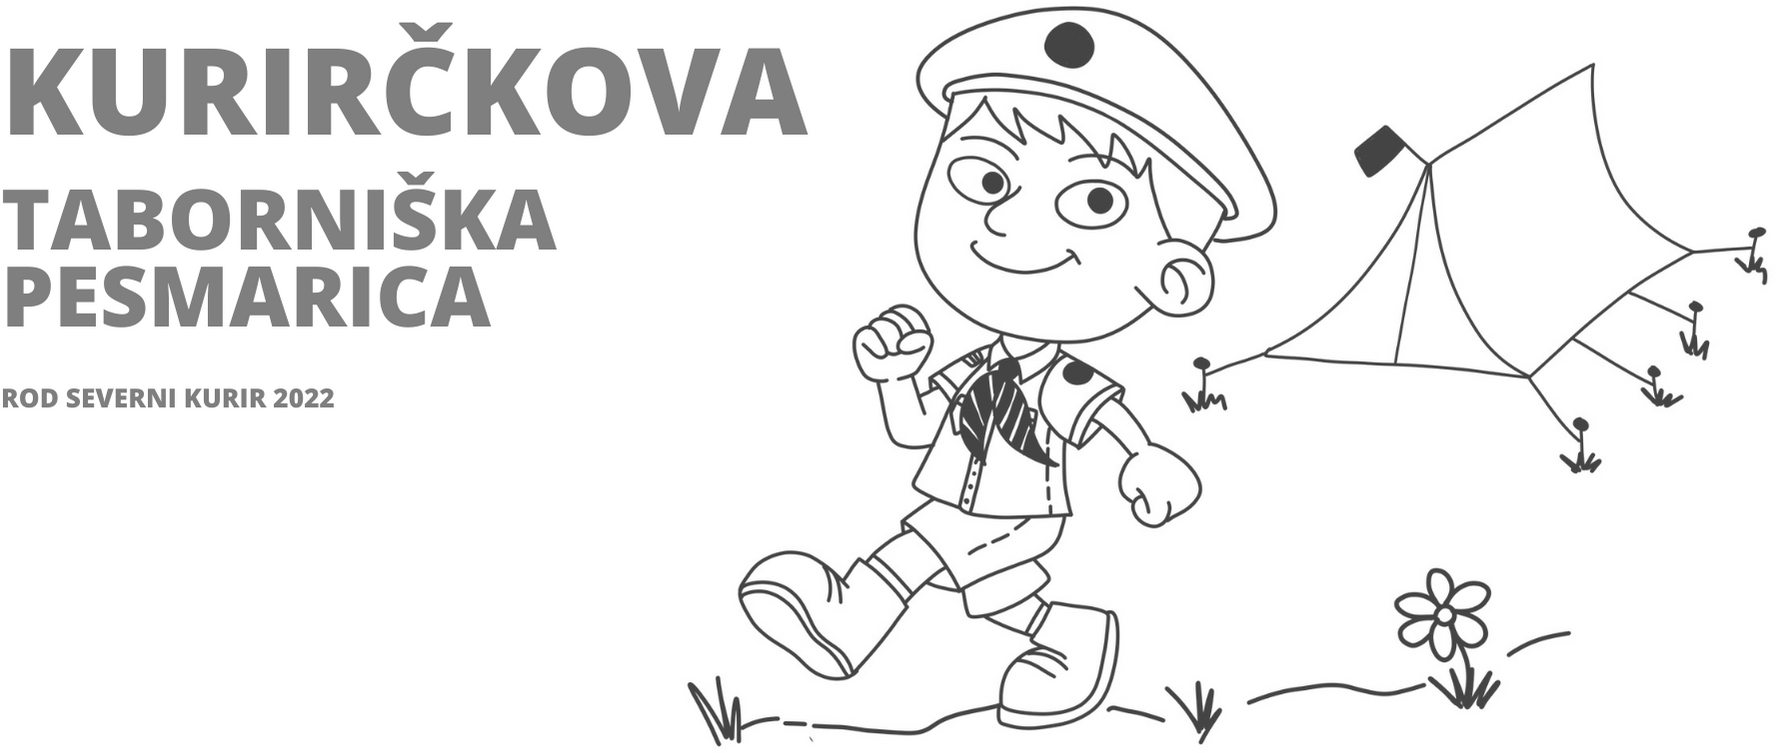
\includegraphics{imgs/naslovnica}
\vfill
\hspace{0pt}
\pagebreak


\clearpage
\null
\thispagestyle{empty}%
\setcounter{page}{0}
\clearpage

%     \layout
    \begin{songs}{}
        %! suppress = MathOperatorEscape
%! suppress = Unicode
%! suppress =
% ----------------------------------------------
\beginsong{Tam ob ognju našem}[by={Taborniška}]
    \beginchorus
        T\[A]am ob ognju našem si sež\[E]emo v \[E7]roke,
        Plamen neugašen nam je s\[A]rce.
        Vedno te bom lju\[A7]bil, dih gozda, \[D]šum voda,
        Tu je m\[A]oj dom in vedno b\[E]om, tukaj ra\[E7]d osta\[A]l doma.
    \endchorus

    \beginverse
        K\[A]akor lepe sanje spomin b\[E]o na te\[E7] dni,
        Ko se spomnim nanje, srce vzdr\[A]hti.
        Saj mladost je naš\[A7]a, kot lepa \[D]majska noc,
        Vsak dan \[A]bo lep spomin kra\[E]san, vedno \[E7]lep in \[A]vedno vroč.
    \endverse
\endsong{}

% ----------------------------------------------
\beginsong{Taborniška himna}[by={Taborniška}]
    \beginverse
        Dviga p\[C]lamen se iz \[G]ognja,
        taboriš\[G7]ca naše\[C]ga,
        ki pod \[F]goro mirno spa\[C]va,
        sredi g\[G7]ozda temneg\[C]a.
    \endverse

    \beginverse
        Tam šotori se blestijo,
        prapor sredi njih vihra
        in oznanja vsej prirodi,
        kje je tabornik doma.
    \endverse

    \beginverse
        Poslušajte bratje sestre
        gozda jelovega spev,
        pesem velike prirode,
        tihi gorski njen odmev.
    \endverse
\endsong{}

\beginsong{Abel in Kajn}[by={Vlado Kreslin}]
    \beginverse
        \[E]Sence so zg\[C#m]inle,
        \[A]težko je zas\[E]pat,
        \[E]jutri pa z n\[C#m]jimi
        \[A]moral bom vst\[E]at.
        \[E]Zdaj tvoje pi\[C#m]smo
        \[A]jemlje mi s\[E]an,
        \[E]pod pouštrom ga skr\[C#m]ivam,
        \[A]dela se d\[E]an. \[C#m]
    \endverse

    \beginchorus
        \[C#m]Ni nama \[A]šlo.
        Bila sva \[C#m]kot Abel in \[A]Kajn.
        \[C#m]Morda pa na \[A]drugem sve\[D]tu
        \[A]nama bo fa\[E]jn. \[C#m]\[A]
    \endchorus

    \beginverse
        \[E]Vzemi me s \[C#m]sabo,
        \[A]daj me v spo\[E]min,
        \[E]tam so že na\[C#m]jine sanje,
        \[A]reka in mlin\[E].
        \[E]Včasih se ze\[C#m]mlja strese
        \[A]in umiri,   \[E]
        \[E]včasih ječi\[C#m]jo breze.
        \[A]Takrat bo\[E]li. \[C#m]
    \endverse

        \beginchorus
        \[C#m]Ni nama \[A]šlo.
        Bila sva \[C#m]kot Abel in \[A]Kajn.
        \[C#m]Morda pa na \[A]drugem sve\[D]tu
        \[A]nama bo fa\[E]jn. \[C#m]\[A]
        \endchorus

\endsong{}

\beginsong{Ako su to bile laži}[by={Plavi orkestar}]
    \beginverse
        \[A]Život ide dalje, život brzo prola\[Bm]zi,
        al' osjećam d\[E]a \[D] to više nisi \[A]ti, a ni \[E]ja.
        \[A]Možda bi i mogli pokušati pono\[Bm]vo,
        al' bojim se d\[E]a \[D] ovaj je \[A]put gotov\[E]o.
        Jer samo \[Bm]ti mi ubrz\[D]avaš disa\[E]nje,
        jer se \[Bm]ja još uvijek \[D]palim na te\[E]be.
    \endverse

    \beginchorus
        \[A]Ako su to samo bile \[Bm]laži,
        laž\[E]imo se \[D]bar još \[A]malo.\[E]
        \[A]Ako su to samo bile \[Bm]varke,
        varaj\[E]mo se,\[D] varaj\[A]mo.(Ti i\[E] ja)
    \endchorus

    \beginverse
        \[A]Život ide dalje, život brzo prola\[Bm]zi,
        al' osjećam d\[E]a to više n\[D]isi t\[A]i, a ni \[E]ja.
        \[A]Ljubavi i mržnje, teško je preskočiti z\[Bm]id
        al' bojim se \[E]da d\[D]obar smo p\[A]ar bili \[E]mi.
        Jer samo ti m\[Bm]i ubrza\[D]vaš disanje, \[E]
        jer se j\[Bm]a još uvijek pa\[D]lim na teb\[E]e.
    \endverse

    \beginchorus
        \[A]Ako su to samo bile \[Bm]laži,
        laž\[E]imo se \[D]bar još \[A]malo.\[E]
        \[A]Ako su to samo bile \[Bm]varke,
        varaj\[E]mo se,\[D] varaj\[A]mo.(Ti i\[E] ja)
    \endchorus
\endsong

\beginsong{Bela snežinka}[by={Veter}]
    \beginverse
        \[A]Ko sem te vprašal:Me ljubiš?
        si mi zmajala z glav\[Bm]o,
        rekla mi nisi besed\[E]e,
        čakal zaman sem to\[A].
    \endverse
    \beginverse
        \[A]Sivi oblaki na nebu,
        jasno nebo so zas\[Bm]trli,
        bela snežinka, ki pa\[E]da,
        glej, prvi sneg. \[A]
    \endverse
    \beginchorus
        \[A]Sneg je,
        glej zunaj sn\[Bm]eg je,
        morda se s\[E]pomniš
        še enkrat na m\[A/A7]e. \rep{2}
    \endchorus

    \beginverse
        \[D]Bela snežinka,
        ki \[A]pada spominja me n\[E]ate
        in na vse tiste \[A]dni n\[D]oč\[A]i.
    \endverse
\endsong


\beginsong{Bicikl}[by={Leteči potepuhi}]

    \beginverse
    \nolyrics{ Uvod: \[G]-\[G]-\[G]-\[G] }
        Ukr\[G]adu sem bicikel pofarbu sem ga mal,
        s pl\[C]ave na rumeno, da navjo me spoznal
        sem m\[D]al ga se sfriziru, zdej zgleda kot iz zlata
        mu k\[C]upu še verigo, da lohk zaklenem g\[G]a
    \endverse
    \beginverse
        Ko v\[Em]ozm se po mestu da fr\[D]ajle vidjo me
        drv\[Em]im čez tromostovje pri r\[D]epu srečam te
        me vpr\[Em]ašaš kolk je ura, ne v\[D]em, ker mi stoji
        pa pr\[C]avš, da zlo je važn, ker tolk se ti mud\[G]i.
    \endverse

    \beginchorus
        Vs\[G]ed se gor na štango, bova tk\[A]o hitrej pršla
        dej n\[F]oge bl u luft, da bom lahk prt\[C]isku kar se da
        se c\[G]ela zemlja trese, k\[A]er tolk hitra sva
        je tr\[F]eba počasnej ej e\[C]j, da nav guma počil\[G]a.. (o jaa)
    \endchorus
    \beginverse
        Pr rep\[G]ubliški upravi čez rdečo peljeva
        poli\[C]caj naju ustavi in me oklofuta
        nik\[D]oli u ta rdečo, boš spendrekom dobil
        nar\[C]edu bos nesrečo, če bos u ta rdečo ri\[G]l.
    \endverse

    \beginverse
        Vse s\[Em]orte me sprašuje, trd\[D]i da sem pijan
        še t\[Em]ebe nadleguje, ker nadl\[D]ežen je organ
        vpr\[Em]aša za bicikl in z l\[D]ukno mi grozi
        t\[C]i si pa čist že živčna, ker tolk se ti mudi\[G]!
    \endverse
    \beginchorus\baselineskip=14pt
        (Refren 2x)
    \endchorus
\endsong





\beginsong{Strel v koleno}[by={Mi2}]
    \beginverse
        \[Em]Kdo si, \[C9]kakšna, k\[Asus2]aj počneš,
        \[Em]za vrati \[C9]kamor jaz ne \[Asus2]smem?
        \[Em]Čeprav jih \[C9]na stež\[Asus2]aj odpreš,
        \[Em]vkopan os\[C9]tanem tu kjer \[Asus2]sem. \[A5] \[H5]
    \endverse

    \beginverse
        \[C]Ker pač nisem\[G] zmagovalec,
        \[Hm]ki vzame to, \[Asus2]kar mu je všeč. \[A5] \[H5]
        \[C]Grajskih stolpov\[G] osvajalec,
        \[Hm]iskri vranec, ostri m\[D]eč.
    \endverse

    \beginchorus
        Kot princ\[G]eskam pristoji,
        ti zab\[F]odeš prst v vreteno.
        Princ pren\[Am]ese več krvi,
        izbere r\[Cm]aje strel v koleno. \rep{2}
    \endchorus

    \beginverse
        \nolyrics{\[Em C9 Asus2]} \rep{2}
        \[Em]Ne jemlji \[C9]tega k\[Asus2]ot poraz.
        \[Em]Ne obupaj\[C9] nad poz\[Asus2]abo.
        \[Em]Pravljic\[C9]e za kr\[Asus2]atek čas
        \[Em]niso z\[C9]a vsakd\[Asus2]anjo rabo.\[A5] \[H5]
    \endverse

    \beginverse
        \[C]Niti večni\[G] ponavljalec,
        \[Hm]ki ga sonce oslep\[Asus2]i. \[A5] \[H5]
        \[C]Mali zlati\[G] prinašalec.
        \[Hm]Pomaha z repom, ko \[D]zbeži.
    \endverse

    \beginchorus\baselineskip=14pt
        Refren \rep{2}
    \endchorus

    \beginverse
        \[C]Ker pač nisem\[G] zmagovalec,
        \[Hm]ki vzame to, kar mu je vš\[D]eč.
    \endverse

    \beginchorus\baselineskip=14pt
        Refren \rep{1}
    \endchorus
\endsong


\beginsong{Bit (Smisel življenja)}[by={Zmelkoow}]
    \beginverse
        \[D]Zadeli smo filozofijo v čelo
        \[D#]našli smo \[B]bit okroglo in d\[A]ebelo
        \[D]se je skrivala na otoku sredi oceana
        \[D#]s sladoledom \[B]v roki \[E]vsa nasme\[A]jana
        \[D]o bit ti nesrečna zakaj si se skrila
        \[D#]ko te ni b\[B]lo je svet \[E]zmeda pre\[A]krila
        \[D]ljudje levo desno brezglavo hitijo
        \[D#]smisla in b\[B]istva si s\[E]rčno žel\[A]ijo
        o, \[DDD]bit \[C]usm\[D]il\[C]i \[D]se \[F]nas\[D#] in pove\[B]]j enkrat za \[E]vselej na \[A]glas
        kaj je \[D]smise\[D]l in \[D]namen k\[C]ako\[D] j\[C]e \[D]treba \[F]živet
        da bomo \[D#]srečni in \[B]zdravi od \[E]glave do \[A]pet
    \endverse

    \beginchorus
        \[h]smisel življenja je \[E]ležanje na plaži z mož\[A]gani na off in \[D]čiwawo na \[A]straži
        \[h]visenje v mreži med \[E]dvemi drevesi, \[A]slalom v ravnini z zarja\[D]velimi ko\[A]lesi
        \[h]smisel življenja je \[E]jahanje oblakov \[A]pihanje v sonce in \[D]lomljenje ko\[A]rakov
        \[h]sanjanje parnika na \[E]modrem ogledalu \[A]piknik z mravljico in \[D]luknja v san\[A]dalu
    \endchorus
    \beginverse
        \[D]Zadeli smo filozofijo v čelo
        \[D#]našli smo \[B]bit \[E]okroglo in d\[A]ebelo
        \[D]se je skrivala na otoku sredi oceana
        \[D#]s sladoledom \[B]v roki \[E]vsa nasme\[A]jana
        \[D]kasneje je priznala da je že nekaj spila
        \[D#]in da\[B] sta z aristi\[E]pom enega\[A] prej pokadila
        \[D]vseeno se ni zmedla in je še enkrat ponovila
        \[D#]modri na\[B]svet in \[E]plava navo\[A]dila
    \endverse
    \beginchorus\baselineskip=14pt
       Refren \rep{2}
    \endchorus
\endsong

\beginsong{Bil je konjenik}[by={Taborniška}]
    \beginchorus
        \[C]Bil je konjenik na iskrem črnem vrancu,
        jahal je skoz noč kot blisk in kot vihar.
    \endchorus
    \beginverse\baselineskip=15pt
        Konjeniki, pozor!
        z levo roko / desno roko
        z levo nogo / desno nogo
        z glavo / jekizkom / celim telesom

        (vmes se poje refren)
    \endverse
\endsong


\beginsong{Bog ne daj da bi crknu TV}[by={Adi Smolar}]
    \beginverse
        \[D]Kadarkoli naša \[G]je družina zbrana
        \[A]se razporedimo \[G]okol TV ekrana.
        Pet nas je, vsi molče sedimo,
        gledamo program, nič ne govorimo. \baselineskip=14pt
        Se noben na nobenga ne ozira
        in zato ne pride do prepira.
        Vsi smo v svoje misli zatopljeni,
        prav lepo, lepo smo odtujeni
    \endverse

    \beginchorus
        \[D]Bognedaj, da bi \[G]crknu televizor, \[A]bognedaj \[G] \rep{4}
    \endchorus

    \beginverse
        \baselineskip=14pt
        Starejše sestre nobeden ne pogleda,
        sreča njena, saj je čisto bleda.
        Trebuh njen se počasi veča,
        s poročenim šefom že dolgo je noseča.
        Se v fotelj ta mlajša je skrila,
        malo prej je travco pokadila.
        Jo v mamila družba je zavedla,
        šprica šolo, totalno je zabredla.
    \endverse

    \beginchorus
    \[D]Bognedaj, da bi \[G]crknu televizor, \[A]bognedaj \[G] \rep{4}
    \endchorus

    \beginverse
        \baselineskip=14pt
        Fotra je sanacija zadela,
        rekli so, da bo ostal brez dela.
        Mat' molči, ker noče biti tečna,
        a v zakonu že dolgo ni več srečna.
        če bi se odkrito kdaj pogovorila,
        bi takoj, takoj bi se ločila.
        Jaz molčim, a kaj bi jih sekiral,
        da na faksu totalno sem sfaliral.
    \endverse

    \beginchorus
    \[D]Bognedaj, da bi \[G]crknu televizor, \[A]bognedaj \[G] \rep{4}
    \endchorus

    \beginverse
        \baselineskip=14pt
        Kadarkoli naša je družina zbrana
        se razporedimo okol TV ekrana.
        Pet nas je, vsi molče sedimo,
        gledamo program, nič ne govorimo.
        Se noben na nobenga ne ozira
        in zato ne pride do prepira.
        Vsi smo v svoje misli zatopljeni,
        prav lepo, lepo smo odtujeni
    \endverse

    \beginverse
        \[D]Kaj zato, če \[G]čisto nič ne štima,
        \[A]ob televizorju \[G]srečna smo družina.  \rep{4}
    \endverse

\endsong


\beginsong{Bor do bora}[by={Taborniška}]
    \beginverse
        \[C]Bor do bora, jelka z \[G]jel\[G7]ko,
        Kakor gora, kakor j\[C]eklo,
        Rod do roda, vsi \[C7]v dru\[F]žini,
        Smo v svob\[C]odni d\[G]omo\[G7 C]vini. \[C7]
    \endverse

    \beginchorus
       S\[F]ile močne, \[C]sile sile čvrste,
        \[G]strnjen\[G7]e so v \[C]naše v\[C7]rste,
        \[F]Sile močne, s\[C]ile sile čvrste,
        \[G]Naše v\[G7]rste \[C]so!
    \endchorus

    \beginverse
        \[C]Šotor dom, narava  \[G]ma\[G7]ti
        Oče grom, gozdovi br\[C]ati
        Od sestra pl\[C7]anin na m\[F]orje
        Širi, š\[C]iri \[G]se ob\[G7]zorj\[C]e. \[C7]
    \endverse

    \beginchorus\baselineskip=14pt
        (Refren)
    \endchorus

    \beginverse
        \[C]Glas severa, juga p\[G G7]esem
        Tisočera v svet pon\[C]ese
        Taborno nam g\[C7]eslo p\[F]ravo
        Hej, tab\[C]orniki\[G] v na\[G7 C]ravo. \[C7]
    \endverse

    \beginchorus\baselineskip=14pt
        (Refren)
    \endchorus
\endsong







\beginsong{Bratovšina sinjega galeba}[by={Film}]
    \beginverse
        \[C]Pesem v vodah izgublj\[Dm]eno
        \[G]plima prinaša na pl\[C]an.
        \[C7]Trka na srca,\[F] da gremo
        \[D7]poslušat jo noč\[G] in dan.
    \endverse

    \beginverse
        \[F]Morje se zgodaj preb\[C]uja,
        \[F]preden rodi se  sv\[C]it,
        \[Am]ribice zlate ponuja,
        \[G]pridi jih srečnež lovit.
    \endverse


    \beginchorus
        \[C]Mi vstajamo, jadramo,
        \[A7]kakor ga\[Dm]lebi na pot.
        \[G]V dalji ostajajo
        \[Dm]pusti o\[G]toki z\[C]mot.
    \endchorus

    \beginverse
        \[C]Mostove postavljamo,
        \[C7]družno od brega na \[F]breg.
        \[C]V sr\[H7]eči, \[A7]ki vsi jo saanjaamoo
        \[Dm]plove naš s\[G7]inji gale\[C]b. \rep{2}
    \endverse
\endsong


\beginsong{Sonce sije veter brije}[by={Taborniška}]


    \beginchorus
        \[Am]Sonce sije, \[F]veter brije, \[C]tebe pa n\[G]i.
        \[Am]Kod hodiš, \[F]kje se skriv\[C]aš, kje si \[G]mi ti?
    \endchorus

    \beginverse
        \[Am]Na dolgo pot grem z\[F]daj,
        \[C]ne bo me več \[G]nazaj.
        \[Am]In nič ne vprašaš z\[F]akaj,
        \[C]zakaj tako sed\[G]aj.
    \endverse

    \beginchorus\baselineskip=14pt
        (Refren)
    \endchorus

    \beginverse
        \[Am]Po polju sva šla, \[F]
        \[C]zvezde gledal\[G]a.
        \[Am]Čakala pomlad,  \[F]
        \[C]predaleč je b\[G]ila.
    \endverse

    \beginchorus\baselineskip=14pt
        (Refren)
    \endchorus

    \beginverse
        \[Am]Odhajam zdaj\[F],
        \[C]ne bo me več \[G]nazaj.
        \[Am]Kaj boš pa sedaj\[F]?
        \[C]Izgubila boš \[G]ta raj!
    \endverse


    \beginchorus\baselineskip=14pt
        (Refren)
    \endchorus

% TODO: spremenit na gornji kot?
    \beginverse
        \[Am]V Stavčo vas grem z\[F]daj,
        \[C]ne bo me več \[G]nazaj.
        \[Am]Še vprašaš zaka\[G]j,
        \[C]ker tam imam \[G]svoj raj. Misl'm kaj?

    \endverse


    \beginchorus\baselineskip=14pt
        (Refren)
    \endchorus

\endsong



\beginsong{Brez obžalovanj}[by={Mi2}]
    \beginverse
        \[E] kdaj si zadnjič šel nar\[E]obe
        \[Am] v prepričanju da stopaš pr\[E]av
        \[E] kdaj z najboljšimi nam\[C#m]eni
        \[Am] slepil lagal in goljuf\[F#m]al
    \endverse

    \beginverse
        \[C#m]vrni ves dolg in pl\[A]ačaj obresti
        na vs\[C#m]ak,  prehojen  kor\[B]ak....... \[A G#m FR#m E]
    \endverse


    \beginchorus
        \[E] brez obžalov\[B]anj
        \[Am] na križišču s\[C#m]anj
        \[E] brez objokova\[B]nj
        \[Am] na križišču s\[E]anj
    \endchorus

    \beginverse
        \[E] kdaj nazadnje stisnil z\[E]obe
        \[Am] namesto da bi zakrič\[E]al
        \[E] kdaj prehitro dvignil r\[C#m]oke
        \[Am] in se že v naprej pred\[F#m]al
    \endverse

    \beginverse
        plj\[C#m]uni na vraže pog\[A]asi grmado
        odž\[C#m]eni se str\[B]an....... \[A G#m F#m E]
    \endverse

    \beginchorus\baselineskip=14pt
        (Refren)
    \endchorus

    \beginverse
        \[C#m] včasih pa lahk\[A]o priznaš
        \[B] se potegneš č\[E]isto vase
        \[C#m] pustiš da mah oč\[A]i prerase
        \[B] in za trenutek\[E] kar umreš

    \endverse

    \beginverse
        \[A] takrat ko naprej ne znaš
        \[C#m] in ne verjameš v nove čase
        \[B] drži se in \[Am]... pazi nase (Refren)
    \endverse
\endsong


\beginsong{Cela ulica nori}[by={Kingston}]
    \beginverse
        \[G]Nocoj ne rab\[C]iš pižame, \[D]
        \[G]in ne veli\[C]kih besed. \[D]
        \[G]Ne razme\[C]tuj omar, \[D]
        \[G]hej, samo pripra\[D]vi se.
    \endverse

    \beginverse\baselineskip=14pt
    Nocoj ne rabiš pižame
    in dežnika tudi ne.
    Ne zapiraj oken,
    samo prisluhni glasbi z ulice.
    \endverse

    \beginchorus
        \[D]Cela ulica nor\[G]i, (ulic\[C]a nor\[D]i)
        \[D]ne kliči 1-1-\[G]3, (1-\[C]1-\[D]3)
        \[D]cela ulica nor\[G]i, (ulic\[C]a nor\[D]i)
        \[D]je kot morje nem\[G]irno, s\[C]e ti ne zd\[D]i.
    \endchorus

    \beginverse\baselineskip=14pt
        Nocoj ne rabiš pižame
        niti praznih obljub.
        Vzemi le sandale,
        glej cela zemlja gori.
    \endverse

    \beginverse\baselineskip=14pt
        Nocoj naju smeh ne objame
        naj zažarijo oči
        a naj srce se ne vname
        za tatove neprespanih noči.
    \endverse

    \beginchorus\baselineskip=14pt
        (Refren)
    \endchorus

    \beginverse\baselineskip=14pt
        Ko se jutro na okna prikrade
        si zakrivamo oči
        a ko sonce spet v morje pade:
    \endverse

    \beginchorus\baselineskip=14pt
        (Refren)
    \endchorus
\endsong


\beginsong{Čas}[by={Dan D}]
    \beginchorus
        \[C]Čas bo zacelil svet, čas bo pomlajšal ta plan\[F]et
        in ko naju ne bo ostalo bo rožnato neb\[C]o.
        \[C]Čas bo ohranil "good look", vzel bo v usta ves ta hr\[F]up
        in ko naju ne bo ostala bo duša ne tel\[C]o.
        \nolyrics{ \[C]-\[C]-\[C]-\[C] }
    \endchorus

    \beginverse
        \[C]Potovanja od m\[G]isli do misli
        od m\[A]mesta do mesta t\[F]a dolga cesta.
        \[C]Pričakovanja od t\[G]ebe do mene
        od m\[Am]ene do tebe.\[F]
    \endverse

    \beginverse
        \[C]Noči brez spanja dn\[G]evi čakanja
        \[Am]in zrno up\[F]anja.
        \[C]Iskanja drugih nač\[G]inov za isto poč\[Am]etje,
        \[F]srčno vnetje.  (Refren 2x)
    \endverse

    \beginverse
        \[C]Čas bo ohranil "good look", vzel bo v usta ves ta hr\[F]up
        in ko naju ne bo ostala bo duša ne tel\[G]o.
        Čas bo rekel stooo\[F]ooop.
        Čas je še z\[F]a en krog, čas je še z\[F]a en krog...
    \endverse
\endsong


\beginsong{Če si srečen}[by={Otroška}]
    \beginchorus
        \[C]Če si srečen, zdaj udari z dlanjo v d\[G]lan.
        \[G7]Če si sre`en, zdaj udari z dlanjo v dl\[C]an.
        \[F]Če si sre:en in če srečo\[C] rad bi še delil z nekom,
        \[G]če si srečen, zdaj u\[G7]dari z dlanjo v dl\[C]an.
    \endchorus

    \beginverse\baselineskip=14pt
        Če si srečen, s prsti tleskni razigran...
        Če si srečen, po kolenih potrepljaj...
        Če si srečen, krepko z nogo butni v tla...
        Če si srečen, glasno vzklikni svoj hura...
        Če si srečen, zdaj ponovi vse od prej...
    \endverse
\endsong


\beginsong{Čakal sm te ko kreten}[by={Mi2}]
    \beginverse
        \[Am]Čakal sn te c\[C]elo jutro, celo n\[G]oč, večer in dan \[Em]pred tem,
        od nikoder ni bilo korakov,mobitel zaspal je gluh in nem
        Je b’lo res vse tak narobe, da je treba b’lo končat?\baselineskip=15pt
        Kdo bo zdaj prenašal moje fore, kdo smejal se mi od vrat?
    \endverse

    \beginverse\baselineskip=15pt
        Zbrani v vrsti pod zastavo smo verjeli v neke boljše dni,
        gazili bi, jedli travo, brez besed prelili svojo mlado kri,
        za Boga, za domovino, da bi zrušili oblast,
        za šteko čikov, liter vina, pa da malo vbijemo dolgčas.
    \endverse

    \beginchorus
        Čakal sn te ko kret\[C]en,
        čakal neke b\[D]oljše čase,
        \[H]preveč butast, preveč l\[C]en,
        \[D]da bi mogo m\[G]isl’t nase. \rep{2}
    \endchorus


    \beginverse\baselineskip=15pt
        Tamkaj, čisto na začetku,ko je svet še zadnjič bil iskren
        v zavetju materinih prsi,dokler uka žeja ni me gnala ven
        se podvizat, da bi zrasel, se naučil, da bi razumel,
        da čimprej bi znal počet vse tisto, kar kdo drug mislo, da bi h’tel.
    \endverse


    \beginchorus\baselineskip=14pt
        Refren \rep{2}
    \endchorus

    \beginverse
        In sem rinil ko kret\[C]en,
        rinil v neke b\[D]oljše čase,
        \[H]preveč butast, preveč l\[C]en,
        \[D]da bi mogo m\[G]isl’t nase.
    \endverse

    \beginverse\baselineskip=14pt
        Vse življenje ko kreten
        sanjam neke boljše čase,
        slep, da je ves svet v tem,
        kar daš podse, kar daš nase.
    \endverse

    \beginchorus\baselineskip=14pt
        Refren \rep{2}
    \endchorus

\endsong

\beginsong{Čau sonček}[by={Zmelkoow}]
    \beginverse
        Čau\[Am] sonček, kot si h\[C]odil do zdaj?
        Sem se že v\[G]prašal, če te n\[D]e bo več nazaj.
        Sem ved\[Am]no vedel, da boš \[C]živel dlje kot jaz,
        ampak te\[G]ga ti ne bom priz\[D]nal.
    \endverse

    \beginverse
        Men\[Am]e obrača okoli tv\[C]oje osi,
        ti se vrt\[G]iš za dobro v\[D]oljo ljudi
        in čisto ve\[Am]dno tisto jutro, \[C]ko me zjutraj zbudiš,
        se lažje\[G] diha, ko se\[D] neha i\[Am]z dimnikov kadit
    \endverse


    \beginchorus
        \[Am]Čau sooonček, kot si hodil do zd\[G]aj? \[D]
        \[Am]Čau sooonček, vrni se naz\[G]aj! \[D]
        \[Am]Čau sooonček, danes ni dobro biti mr\[G]tev. \[D]
        \[Am]Čau sooonček, pa kaj mrtev, še pij\[G]an, preveč pi\[D]jan.
    \endchorus

    \beginverse
        \[Am]Ko mimo mene blodi g\[G]mota ljudi,
        je prav za\[G]bavno videt \[D]toliko laži,
        \[Am]toliko neumnih motivov in \[C]neumnih zarot,
        sonček d\[G]ej ne se ozirat in s\[D]veti rajši drugod.
    \endverse

    \beginchorus\baselineskip=14pt
        Refren
    \endchorus
\endsong



\beginsong{Če bi se midva kdaj srečala}[by={Vlado Kreslin}]
    \beginchorus
        \[A]Če bi midva  se kdaj\[E] srečala
        \[D]v kratki zgodbi prem\[E]ajhni za dva
        \[A]Če bi midva  se kdaj\[E] srečala
        \[D]kot roman ki se sreč\[E]no konča
    \endchorus

    \beginverse
        \[Hm]enkrat ob petih popo\[D]ldne  tam dol pred bifejem
        \[A]takrat ko se služba \[E]konča
        \[Hm]v tistem črnem  kost\[D]imu  in  petkah
        \[A]lahkotna kot srna   \[E]bi  mimo prišla
    \endverse

    \beginverse\baselineskip=14pt
        Če bi midva se kdaj srečala
        in bi muzika špilala
        Če bi midva se kdaj srečala
        tisti večer usoden za oba
    \endverse

    \beginchorus\baselineskip=14pt
        ti bi v kotu sedela z najboljšo prijateljco
        pila bi tonik in džin
        mi pa še en dodatek in folk ves navdušen
        jaz pa neroden in fin
    \endchorus

    \beginverse\baselineskip=16pt
        \nolyrics{ \[A E D E] } \rep{2}
        \nolyrics{ \[Hm D A E] } \rep{2}
    \endverse

    \beginverse\baselineskip=14pt
        Če bi midva se kdaj srečala
        a bi bil ta osamljenn večer
        Če bi midva se kdaj srečala
        a imela bi sina al hčer
    \endverse

    \beginchorus\baselineskip=14pt
        A bi zdajle pel ta samotni napev
        tole majceno pesem za dva
    \endchorus

    \beginchorus\baselineskip=14pt
        bi se zunaj temnilo in rahlo rosilo
        in bil bi večer kot je zdaj \rep{3}
    \endchorus

    \beginchorus\baselineskip=14pt
        bi se zunaj temnilo in rahlo rosilo
        Če bi midva se kdaj srečala...
        \[A]kdaj srečala
    \endchorus
\endsong

\beginsong{Čez tisoč let}[by={Vlado Kreslin}]
    \beginverse
        Tisto n\[Am]oč, ko sva šl\[C]a,
        dvigni\[G]la si me z dna do neb\[D]a,
        dala mo\[Am]č, ki jo d\[C]a
        nekdo, \[G]ki te upošteva, rad im\[D]a.
    \endverse

    \beginverse
        Je to m\[Am]alo ali \[C]vse,
        a zaht\[D]evamo preveč ali pač \[C]nee\[D]ee?
    \enndverse

    \beginchorus
        \[Em] Tudi čez \[G]tisoč l\[D]et tu bom st\[C]al,
        \[Em] sonce bo\[G] moje src\[D]e,
        \[Em] ena od \[G]tisoč zv\[D]ezd mi bo pr\[C]av,
        \[Em] nosil bom nj\[G]eno im\[D]e!
    \endchorus

    \beginverse
        Knjigo, s\[Am]ina in drev\[C]o sem mu d\[D]al,
        zdaj pa hoče še tel\[C]o in \[D]dušo.
    \endverse

    \beginchorus\baselineskip=14pt
        Refren
    \endchorus

    \beginverse
        \[F]In že jutri spet bo t\[C]o,
        kar že včeraj je bil\[G]o. \rep{2}
    \endverse

    \beginchorus\baselineskip=14pt
        Refren
    \endchorus
\endsong

% TODO: preverit akorde
\beginsong{Najlepši od tabornikov}[by={Taborniška}]
    \beginchorus
        \[G]On je najlepši od tabor\[D]nikov,
        želela sem do\[Em]tikov,
        ko mi menaško \[C]je pom\[D]il.
        \[G]Jaz sem poškodbo zaig\[D]rala,
        sem se mu zla\[Em]gala,
        samo da ojgn\[C] kurla \[D]bi.
    \endchorus

    \beginverse
        \[G]Ko prišla sem na sek\[D]ret,
        mi ukradel je pogl\[Em]ed,
        od sramu sem prdn\[D]ila.
    \endverse

    \beginverse
        \[Em]Taborjenje je le\[D]tno,
        res bilo je pri\[C]jetno,
        in njegove s\[D]ladke okice.
    \endverse

    \beginchorus\baselineskip=14pt
        Refren
    \endchorus
\endsong

\beginsong{Najlepši od zdravnikov}[by={Mirna Reynolds}]
    \beginchorus
        \[G]On je najlepši od zdrav\[D]nikov,
        želela sem do\[Em]tikov,
        preveril bitje \[C]je sr\[D]ca.
        \[G]Jaz sem bolezen zaig\[D]rala,
        vse se mu zla\[Em]gala,
        samo da skupaj\[C] sva \[D]bila.
    \endchorus

    \beginverse
        \[G]Ko prišla sem na preg\[D]let,
        mi ukradel je pogl\[Em]ed,
        od sramu sem zard\[D]ela.
        \[G]Pospešil se je moj u\[D]trip,
        trda sem bila kot k\[Em]ip
        in nalašč omed\[D]lela.
    \endverse

    \beginverse
        \[Em]Dihanje ume\[D]tno,
        res bilo je pri\[C]jetno,
        in njegove s\[D]ladke ustnice.
        \[Em]Visoka tempera\[D]tura,
        seksi vroča fi\[C]gura,
        \[D]je začarala me.
    \endverse

    \beginchorus\baselineskip=14pt
        Refren
    \endchorus

    \beginverse
        \[G]Dal mi je injekci\[D]jo
        Kar bolečo lekc\[Em]ijo
        Da sem kar zakri \[D]čala
        \[G]Hitro se je dvigal t\[D]lak
        V sobi je zavladal \[Em]mrak
        Celo noč sva osta\[D]la
    \endverse

    \beginchorus\baselineskip=14pt
    Refren \rep{2}
    \endchorus

\endsong

\beginsong{Črn tulipan}[by={Big foot mama}]
    \beginverse
        J\[A]est sm bog ljubezni, men' ne manjka sanj
        Jest začaram srečo, men' zaupi dlan. \[Hm]
        J\[A]est poznam svetlobo, ki odpira dan
        Z njo si fila žile črn tulip\[D]aaa\[Hm]aan
    \endverse

    \beginverse
        \[A]Ona sanja sonce, čist, kristalen dan
        Nanjo vsake tolk' pristane Peter Pan \[Hm]
        V nj\[A]ej je dost ljubezni, mnogo več krvi
        Nevidna je v temi, prozorna med ljudm\[D]iii j\[Hm]aaa
    \endverse

    \beginchorus
        \[F#m]Zato pa raste t\[Hm]ulipan, \[E]črn divji t\[F#m]ulipan \rep{4}
    \endchorus

    \beginverse
    J\[A]est sm bog ljubezni, men' ne manjka sanj
    Jest začaram srečo, men' zaupi dlan. \[H]m
    J\[A]est poznam svetlobo, ki odpira dan
    Z njo si fila žile črn tulip\[D]aaa\[H]maaan
    \endverse

    \beginchorus\baselineskip=14pt
    Refren \rep{4}
    \endchorus

    \beginverse
        V\[F#m]edno, ko posije č\[Hm]rn tulipan
        T\[E]ol'krat tud' izgine \[F#m]iskra mojih sanj
        Vč\[F#m]asih se pokaže t\[Hm]a škrlaten dan
        D\[E]a začara srečo č\[F#m]rn tulipan.
    \endverse

    \beginverse
        \[G#m]Črrrn t\[C#m]uuuliiip\[F#]aaa\[G#m]aaan
        \[G#m]Črrrn t\[C#m]uuuliiip\[F#]an an \[G#m]ajajajajajaj
        \[G#m]Črn, črn, č\[C#m]rn, črn, č\[F#]rn tulip\[G#m]aaan
        \[G#m]Črrrn t\[C#m]uuuliiip\[F#]an an \[G#m]aaan
    \endverse

\endsong


\beginsong{Čez šuštarski most}[by={Majda}]
    \beginverse
        V Ljublj\[C]ani za Ljublj\[E7]anico, tam n\[Am]ajde vsak vse, k\[C7]ar želi,
        tam skr\[F]ije med cvetl\[C]ice te J\[D7]lija b\[G7]ar.
        Če s\[C]i zaljubljen, č\[E7]e si mlad, \[Am]a čez leto \[C7]in čez dan
        priš\[F]el boš tja z nev\[C]esto n\[Dm]a mag\[G7]istra\[C]t.
    \endverse

    \beginchorus
        Č\[C]ez Š\[E7]uštarski m\[Am]ost,           \[C7]
        č\[F]ez Š\[C]uštarski m\[D7]ost,           \[G7]
        l\[C]evo na M\[E7]estni trg, d\[Am]esno na St\[C7]ari trg,
        p\[F]o spomine, p\[C]o mladost čez Š\[Dm]uštarsk\[G7]i mos\[C]t.
    \endchorus


    \beginverse
        V Ljublj\[C]ani za Ljublj\[E7]anico n\[Am]ajde vsak, kar \[C7]išče,
        tam z\[F]a večerjo V\[C]itez kop\[D7]una ti d\[G7]a
        in M\[C]aček cvička rd\[E7]ečega in če z m\[Am]ačkom greš od t\[C7]am,
        lahk\[F]o potunkaš gl\[C]avo v R\[Dm]obbov v\[G7]odnja\[C]k.
    \endverse

    \beginchorus\baselineskip=14pt
    Refren
    \endchorus

    \beginverse
        V Ljublj\[C]ani za Ljublj\[E7]anico, tam n\[Am]ajde vsak, kar \[C7]išče,
        fant s\[F]ulico, mož cv\[C]iček in l\[D7]una balk\[G7]on,
        najv\[C]ečjo knjigo \[E7]učenjak, m\[Am]inikrilo d\[C7]eklica,
        še t\[F]ole svojo p\[C]esem n\[Dm]ašla s\[G7]em ta\[C]m.
    \endverse

    \beginchorus\baselineskip=14pt
        Refren
    \endchorus
\endsong


\beginsong{Sentiš navadni}[by={Zmelkoow}]
    \beginverse
        \[C]Ko si dobra, ko se po\[Gm]skušas upirat in upaš, da ti\[Dm] ne bom verjel, \[Fm]
        \[C]ko skrbno skrivaš svo\[Gm]je misli, ne bom ti \[Dm]jih vzel\[Fm].
        \[C]Dosti prelep\[Gm]a, da bi b'la hudobna, kot hočeš bit,\[Dm Fm]
        \[C]mogoče \[Gm]sva si prepodobna, da te ne bi razumel.\[Dm C']
    \endverse

    \beginchorus
        \[Am]Ne skrivaj \[C]se, ne morem v\[Gm]eč, \[Dm]
        \[Am]ne beži \[C]mi, rad bi \[Gm]probal s tabo umret. \[Dm]
        \[Am]Ne dvomi \[C]zdaj, nimam mo\[Gm]či, da bi lagal \[Dm]
        \[Am]ne umikaj \[C]se, rad bi t\[Gm]e samo držal. \[Dm]
    \endchorus
    \beginchorus
       (vse 2x),  (Pol tona nižje, refren in C': barre)
    \endchorus
\endsong


\beginsong{Čista jeba}[by={Mi2}]
    \beginchorus
        \[D]Čista \[Dmaj7]jeba, to \[D]je č\[Dmaj7]ista jeba
        \[G]Ko si hkrati čisto blizu \[Em]pa tak daleč \[A]od vsega
    \endchorus

    \beginverse
        \[D]Ko bi vedla, k\[Dmaj7]o bi znala \[D]tisto noč bi r\[Dmaj7]aje spala
        \[F#m]tiho zlekljena vsak sebi \[G]brez spoznanj o čisti jebi.
        \[D]A usoda j\[Dmaj7]e hotela \[D]da predolgo st\[Dmaj7]a trpela
        \[F#m]Njega grozno je dajalo \[G]ko je gledal sladko Zalo
        \[Hm]Ona pa je h\[F#m]odla k maši, \[G]a pri maši \[D]mašnik str\[F#m]aši
        \[Hm]Kdor v življenju vz\[F#m]držen ne bo \[E]si nakoplje č\[A]isto jebo.
    \endverse

    \beginchorus\baselineskip=14pt
        Refren \rep{2}
    \endchorus

    \beginverse
        \[D]Tak so jima t\[Dmaj7]ekla leta, \[D]v nauku duha s\[Dmaj7]ina očeta
        \[F#m]Ni več dvoril, ni več upal, \[G]v žganju tiho je obupal
        \[D]Ko je končno l\[Dmaj7]e izbrala \[D]pamet pred lažn\[Dmaj7]o moralo
        \[F#m]Dedec je uvidel zgrožen \[G]da ni v gatah nič več prožen
        \[Hm]Spomni se kaj gn\[F#m]ħal je pater \[G]pošlje vse v b\[D]ožjo m\[F#m]ater
        \[Hm]in si gre z rok\[F#m]o nad sebe \[E]bil je konec č\[A]iste jebe
    \endverse

    \beginchorus\baselineskip=14pt
        Refren \rep{2}
    \endchorus

    \beginverse
        \[Hm]Nauk teh zgodbic l\[F#m]e nam pravi, \[G]da zaupaj sv\[D]oji gl\[F#m]avi
        \[Hm]Saj že brez modr\[F#m]osti smeha \[E]je življenje č\[A]ista jebaaa\[H]a...
    \endverse

    \beginchorus\baselineskip=14pt
        Refren
    \endchorus
\endsong



\beginsong{Čuk se je oženil}[by={Otroška}]
    \beginchorus
        Č\[D]uk se je oženil, tr\[G]alal\[D]a, tr\[G]alal\[D]a,
        s\[A]ova ga je vz\[D]ela, h\[A]opsas\[D]a,
        s\[A]ova ga je vz\[D]ela, h\[A]opsas\[D]a.
    \endchorus
    \beginverse\baselineskip=15pt
        Čuk sedi na veji, tralala,
        sova na vereji, hopsasa!
        Sova čuku miga, tralala,
        dajva se, vzemiva, hopsasa!
        Čuk pa sovo vpraša, tralala,
        kol’ko dota znaša, hopsasa!
        Eno bučo vina, tralala,
        en’ga petelina, hopsasa!
        Vino bova spila, tralala,
        bučo pa razbila, hopsasa!
    \endverse
\endsong

\beginsong{Daleč je za naju pomlad}[by={Adi Smolar}]
    \beginverse
        \[Am]Danes stara sva in s\[Dm]iva, \[G]pozna se težko bre\[C]me let.
        \[E]Postala sva t\[Am]ako ranljiva,\[F]mnogo prehiter je za n\[E]aju svet
        \[Am]Najine p\[Dm]oti so kratke, \[G]le redkokdaj še gre\[C]va kam.
        \[Am]Vedno skupaj, v\[Dm]edno sama. \[F]Ona vs\[E]e je, kar ima\[Am]m!
    \endverse

    \beginchorus
        \[Am]Daleč, daleč je za n\[Dm]aju pomlad, \[G]leta prinesla so jese\[C]n.
        \[Am]Daleč, ko dekletu s\[Dm]em govoril: rad te ima\[G]m, in ko bil jaz fant sem nje\[C]n.
        \[Am]Daleč,daleč je za n\[Dm]aju pomlad,m\[G]i za mladostjo je hudo\[C]
        \[Am]a ne bi hotel sam p\[Dm]ostati spet mlad \[F]raje star sem, star in z njo!\[Am]
    \endchorus


    \beginverse\baselineskip=14pt
        Govoriva si spomine.  Mnogo vsega je bilo.
        Rečeva: kako vse mine, in malo nama je hudo.
        A nato se nasmejiva, srečna, ker sva se našla.
        Kako lepo je, da sva se spoznala in skupaj skozi življenje šla!
    \endverse

    \beginchorus\baselineskip=14pt
        Refren
    \endchorus

    \beginverse\baselineskip=14pt
        Ura prepodi spomine. Greva spat, zašepeta.
        Trdno me pod roko prime in s težavo vstaneva.
        Ponoči k meni se privije, vsak njen dotik - tako poznan
        mi prežene grenko misel: kdo od naju ostal bo sam?
    \endverse

    \beginchorus\baselineskip=14pt
        Refren
    \endchorus
\endsong

\beginsong{Dan ljubezni}[by={Pepel in kri}]
    \beginverse
        \[C]Pusti tisoč dni in tisoč noč\[D]mi, ki jih več n\[F]i,
        če spl\[G]oh ne veš, da so kdaj bil\[C]i.
        \[C]Vzemi le en dan, ki skril si ga tj\[Dm]a na srčno str\[F]an,
        poz\[G]abil ga nik\[G7]oli več ne b\[C]oš.
    \endverse

    \beginverse
        \[F]To je bil tvoj dan ljubezni,najlepši dan,ki ne m\[C]ine nik\[C7]dar
        \[F]Svet živi za dan ljubezni, dan,ki da ti vse in vse ti vz\[C]ame
        Tega nikdar ne v\[G]eš.
    \endverse

    \beginchorus
        Kd\[F]aj pr\[G]iš\[C]el bo zate sp\[F]et ta d\[G]an,
        n\[F]aaaj t\[G]e upan\[C]je ne zapusti.
        L\[F]e z\[G]asp\[C]i, ko jutro t\[F]e zbud\[G]i,
        t\[F]o b\[G]o ljubezni d\[C]an.
    \endchorus


    \beginverse\baselineskip=14pt
        To je bil tvoj dan ljubezni ...
    \endverse

\endsong


\beginsong{Deamons}[by={Imagine Dragons}]
    \beginverse
        When the d\[D]ays are cold; and the c\[A]ards all fold
        And the s\[Bm]aints we see; are all m\[G]ade of gold
        When your dr\[D]eams all fail; and the o\[A]nes we hail
        Are the w\[Bm]orst of all; and the bl\[G]ood’s run stale
    \endverse


    \beginchorus
        \[D]I wanna hide the tr\[A]uth
        I wanna shelter y\[Bm]ou
        But with the beast ins\[G]ide
        There’s nowhere we can h\[D]ide
        No matter what we br\[A]eed
        We still are made of gr\[Bm]eed
        This is my kingdom c\[G]ome
        This is my kingd\[N.C.]om come
    \endchorus

    \beginchorus
        When you feel my heat
        Look into my eyes\baselineskip=14pt
        It’s where my demons hide
        It’s where my demons hide
        Don’t get too close
        It’s dark inside
        It’s where my demons hide
        It’s where my demons hide
    \endchorus

    \beginverse\baselineskip=14pt
        At the curtain’s call; It's the last of all;
        When the lights fade out; All the sinners crawl;
        So they dug your grave; And the masquerade;
        Will come calling out; At the mess you made;
    \endverse

    \beginchorus\baselineskip=14pt
        Don’t wanna let you down
        But I am hellbound
        Though this is all for you
        Don’t wanna hide the truth
        No matter what we breed
        We still are made of greed
        This is my kingdom come
        This is my kingdom come
    \endchorus

    \beginchorus\baselineskip=14pt
        When you feel my heart...
    \endchorus

    \beginchorus\baselineskip=14pt
        \[(D)]They say it’s what you make
        I say it’s up to fate
        It’s woven in my soul

        I need to let you go
        Your eyes, they shine so bright
        I wanna save that light
        I can’t escape this now
        Unless you show me how
    \endchorus
    \beginchorus\baselineskip=14pt
        When you feel my heart...
    \endchorus
\endsong



\beginsong{Dekle moje pojdi z menoj}[by={Vlado Kreslin}]
    \beginchorus
        D\[E]ekle moje, pojdi z men\[D]oj,
        d\[A]ekle moje, pojdi z men\[E]oj,
        d\[E]ol ob reki, v tisti b\[D]eli obleki,
        d\[A]ekle moje, pojdi z men\[E]oj.
    \endchorus

    \beginverse
        Je se zv\[E]ezda, tam na vodi blešč\[D]i,
        zv\[A]ezda, tam na vodi blešč\[E]i?
        Ne, to je v\[E]enec gizdavi na tv\[D]oji glavi,
        to ni zv\[A]ezda, ki se v vodi blešč\[E]i.
    \endverse

    \beginchorus\baselineskip=14pt
        Refren
    \endchorus

    \beginverse
        Je to m\[E]esec, ki tam z roso lež\[D]i,
        m\[A]esec, ki z roso lež\[E]i?
        Ne, to sta n\[E]aj’ni postavi,
        v mehki, r\[D]osni travi,
        to ni m\[A]esec, ki z roso lež\[E]i
    \endverse

    \beginchorus\baselineskip=14pt
        Refren
    \endchorus
\endsong

%TODO: mogoč sam akorde ene kitice dat?
\beginsong{Dobra vila}[by={Tabu}]
    \beginverse
        Vč\[G]asih, ko slon\[H]im ob oknu
        gl\[Em]edam dol ljud\[C]i,
        z\[G]askrbljene, z\[H]amorjene,
        gl\[Em]ave sklonjen\[C]e.
    \endverse
    \beginverse
        \[G]Ona tiho s\[H]olze skriva,
        on je \[Em]ves \[C]na tleh.
        Vs\[G]e bi dala, d\[H]a zanetim
        \[Em]iskrice v oč\[C]eh.
    \endverse
    \beginverse
        A d\[G]ala bi, če b\[H]i postala
        v\[Em]ila za en d\[C]an,
        nj\[G]emu srečo, nj\[H]ej ljubezen,
        k\[Em]omu le nasm\[C]eeeh...
    \endverse

    \beginchorus
        T\[G]ara ta ta, t\[H]ara ta ta, t\[Em]ara ta ta t\[C]a... \rep{2}
    \endchorus

    \beginverse
        N\[G]ihče več ne \[H]objokuje,
        nič v\[Em]eč ni sk\[C]rbi,
        n\[G]asmejano s\[H]once sije
        \[Em]na vse ljud\[C]i.
    \endverse

    \beginverse
        Pa n\[G]aj udari, n\[H]aj se sliši
        gl\[Em]asno iz neb\[C]a,
        pa n\[G]aj prepeva, n\[H]aj odmeva
        p\[Em]esem čudežn\[C]aaa...
    \endverse

    \beginchorus\baselineskip=14pt
        Refren \rep{3}
    \endchorus

    \beginverse
        Sk\[G]ozi okno d\[H]obra vila
        gl\[Em]eda dol ljud\[C]i.
        Bi p\[G]omagala, č\[H]e bi znala
        najti klj\[Em]uč za vse skrb\[C]iii...
    \endverse

\endsong

\beginsong{Ti nisi ta}[by={Mi2}]
    \beginverse
        \[Asus2]Padel je poslednji zastor \[E]najine tragikomedije
        \[C#m]namesto rož le mrtva riba i\[D]n fotodraž iz Azije.
        \[Asus2]Preveč besed, premalo dotikov, \[E]napačnih zvezd, ponesrečenih trikov
        \[C#m]prehitrih gest, prepoznih umikov \[Dsus2]mojih poti in tvojih \[Asus2]mejnikov
    \endverse


    \beginchorus
        \[Asus2]Ti nisi ta, ki prebere moj znak,
        \[E]ti nisi ta, ki ustavi moj vlak.
        \[Dsus2]Ti nisi ta, ki odpihne moj prah,
        \[F]ti nisi ta, ki p\[G]režene moj strah. \rep{2}
    \endchorus

    \beginverse\baselineskip=14pt
        Peskovnik nima več prostora, kompas kaže staro smer,
        vodnjak želja ostaja prazen, konec vojne, živel mir.
        Počasi zbujam se iz teme, tako preprosto je spet vse,
        ob enem žalosten in srečen da mi vseeno je za te.
    \endverse

    \beginchorus\baselineskip=14pt
    Refren \rep{2}
    \endchorus

    \beginverse\baselineskip=14pt
        \[Asus2]Preveč besed, premalo dotikov, \[E]napačnih zvezd, ponesrečenih trikov
        \[C#m]prehitrih gest, prepoznih umikov \[Dsus2]mojih poti in tvojih \[Asus2]mejnikov
    \endverse

    \beginchorus\baselineskip=14pt
    Refren \rep{2}
    \endchorus

\endsong


\beginsong{Djurdjevdan}[by={Bijelo Dugme}]
    \beginverse
        \[Am]prolje\[G]će na moje \[C]rame slijeće,
        \[Dm]đurđevak ze\[Am]leni
        \[Dm]đurđevak zel\[Am]eni s\[F]vima \[G]osim \[Am]meni
    \endverse

    \beginchorus
        eeeej, evo zore, \[Dm]evo zore
        \[Am]bogu da se \[Dm]pomolim
        \[Am]evo zore, \[Dm]evo zore, \[F]eeeej , đurđevdan je
        \[Dm]A ja nisam\[Am]'s onom \[E7]koju \[Am]volim
    \endchorus

    \beginverse\baselineskip=14pt
        drumovi odoše, a ja ostah
        nema zvijezde danice
        nema zvijezde danice, moje suputnice
        ej, kome sada moja draga
        na đurđrvak miriše
        na đurđrvak miriše, meni nikad više.
    \endverse

    \beginchorus\baselineskip=14pt
        Refren
    \endchorus

    \beginverse\baselineskip=14pt
        ej , kome sada moja draga
        na đurđrvak miriše
        na đurđrvak miriše, meni nikad više.
        njeno ime neka se spominje
        svakog drugog dana
        svakog drugog dana osim đurđevdana
    \endverse

    \beginchorus\baselineskip=14pt
        Refren
    \endchorus
\endsong


\beginsong{Eks za ex- ljubico}[by={Adi Smolar}]
    \beginverse
        \[Bm]Danes nabral si bom že \[D]lodec poln omame
        \[A]in čakal, čakal,\[Em] da me objame.
        Odšla je ženska, za njo žalujem,
        namesto solza tolažbo potrebujem.\baselineskip=15pt
        Potikam se iz oštarije v oštarijo,
        jih tolk je, da od hoje noge me bolijo.
        Pa kaj, če bom zapil kar celo plačo,
        kaj mi bo dnar, jaz rabim dans pijačo.
    \endverse

    \beginchorus
        \[Bm]En liter, \[D]dva litra, \[A]trije litri, \[Bm]pir \[F#]in \[Bm  F#]žganje.
        \[Bm]Eks za ex ljubi\[D]co, za lju\[A]bezen in za \[Bm F#]stare \[Bm  F#]sanje.
    \endchorus

    \beginverse\baselineskip=15pt
        In pijem, pijem, vse kar imajo,
        zlijem vase, karkol mi dajo.
        Pamet mi pravi: Hej pazi malo!
        Srce pa: Pij ga, četud te bo pobralo.
    \endverse

    \beginchorus\baselineskip=14pt
        Refren
    \endchorus


    \beginverse\baselineskip=15pt
        Ves svet vrti, vrti se kot za stavo,
        srce nabija mi alkohol v glavo.
        A čutim, da v meni raste sila,
        ne, ne žalost, ne boš me danes zvila.
    \endverse

    \beginchorus\baselineskip=14pt
        Refren
    \endchorus

    \beginverse\baselineskip=15pt
        Popolni temi se približujem,
        Le kje je ona, pijano se sprašujem.
        Morda na Dunaju, morda v Parizu?
        Oj delirij moj, vsaj ti si blizu.
    \endverse

    \beginchorus\baselineskip=14pt
        Refren \rep{2}
    \endchorus

    \beginverse\baselineskip=15pt
        Ko sem pijan, ne žalujem
        ne, ko sem pijan žensk ne potrebujem, ne ne.
        Utopim v želodcu svojo rano,
        Mi je vseeno, vseeno kaj bo z mano.
    \endverse

    \beginchorus\baselineskip=14pt
        Refren \rep{2}
    \endchorus
\endsong


\beginsong{En mali slonček}[by={Taborniška}]
    \beginchorus
        \[C]En mali slonček se je pozibaval
        N\[a7]a paj\[D7]čevini \[G]tam pod drevesom
        \[C]Ko je ugotovil, da stvar je zanimiva
        \[G]Je p\[G7]oklical \[C]še enega slončka.
    \endchorus
    \beginchorus\baselineskip=14pt
        Dva mala slončka... \rep{9.99e100}
    \endchorus
\endsong

\beginsong{Ena pesem}[by={Vlado Kreslin}]
    \beginverse
        Eno p\[Bm]esem, \[F#7]rad bi napisal p\[Bm]esem,\[F#7]
        eno\[Bm]stavno, pr\[A]ijazno, ki bi bila brez sk\[D]rbi,
        \[A7]ki bi ljudi veselil\[D]a,
        ki bi \[A7]se meni dajala \[F#7]moč!
    \endverse

    \beginverse\baselineskip=15pt
        Brez šoferjev, ki skozi šipe grozijo,
        brez slepih, ki pametne učijo,
        praznin, ki z naslovnic dol zro,
        kravat, ki lepo govorijo,
        a taki pesmi je danes težko.
    \endverse

    \beginchorus
        Nekaj pa j\[D]e še takih ljud\[A]i,
        ki se jih \[Em]človek razves\[G]eli,
        nekaj pa \[D]je še takih lj\[A]udi!
    \endchorus

    \beginverse\baselineskip=15pt
        Verjamem, vem, da mi nekoč bo uspela,
        vem, da me takoj bo zadela,
        prijazna bo legla v srce,
        in bo ljudi radostila,
        in bo se sebe potolažila,
        in vsem nam bo dajala moč!
    \endverse
    \beginchorus\baselineskip=14pt
        Refren
    \endchorus

\endsong


\beginsong{Gorska roža}[by={Andrej Šifrer}]
    \beginverse
        \[C]Odšel sem tja kjer je daljši dan, kjer se m\[F]estni svet konč\[C]a.
        \[C]Kjer namesto asfaltnih cest v\[G]odi le steza.
        \[C]Hiše razpršene kot jata pl\[F]ahih jereb\[C]ic,
        čas utripa drugače, če živiš v \[G7]eni od gorskih vas\[C]ic.
    \endverse
    \beginverse
        \[C]Tisti večer sem žganje pil, kot ga p\[F]ije gospod\[C]ar.
        \[C]Bog mi v jezik je dal moči in takr\[G]at sem jo spoznal.
        \[C]Soseda mlada prisedla je srečal nj\[F]ene sem oč\[C]i.
        \[C]Ko smo peli sem jo gledal, kak\[G7]o se mi smej\[C]i.
    \endverse

    \beginchorus
        \[F]Gorska roža č\[C]aka me, \[G]gorska roža da v\[C]rnem se
        \[F]moji Špeli \[C]iz plan\[A]min po\[G]d srcem pustil s\[C]em spomin.
    \endchorus


    \beginverse\baselineskip=15pt
        Brez staršev je a fantov ni, ki bi ženili se v gore.
        Zjutraj gre v tovarno saj z majhno kmetijo pač ne gre.
        Vzljubila me je čeprav sem bil zanjo skoraj še otrok.
        Naučila me je piti meda jaz sem dal ji svojih 18 let.
    \endverse

    \beginchorus\baselineskip=14pt
        Refren
    \endchorus


    \beginverse\baselineskip=15pt
        Od takrat sem pri njej živel na gruntu ob koncu vasi.
        Čez dan kitaro sem igral in ljubil Špelo vse noči.
        Bil opran sem in vedno sit, jedel kruh sem iz njene peči.
        Vstajala je zgodaj na delavski avtobus se vedno mudi.
    \endverse

    \beginchorus\baselineskip=14pt
        Refren
    \endchorus


    \beginverse\baselineskip=15pt
        Ko zadnja košna v kozolcu je čutis hladen že objem
        postajal sem nemiren saj začutil sem jesen in pravi
        o 'dreja poglej okrog zdaj postal si del planin
        o 'dreja jaz se bojim, da nekoc te ne izgubim.
    \endverse

    \beginchorus\baselineskip=14pt
        Refren
    \endchorus


\endsong


\beginsong{No woman, no cry}[by={Bob}]
    \beginchorus
        \[C] No \[C/B]woman no cry\[Am F]
        \[C] No \[F]woman no \[C]cry \[(G)] \rep{2}
    \endchorus

    \beginverse
        \[G]Said said
        \[C]said I \[G/B]remember \[Am]when we used to sit\[F]
        \[C]In the govern\[G/B]ment yard in t\[Am]renchtown\[F]
        Oba obaserving the hypocrites\baselineskip=15pt
        As they would mingle with the good people we meet
        good friends  we had oh - good friend we lost
        - along the way -
        In this bright future you cant forget your past
        So dry your tears I say
    \endverse

    \beginchorus\baselineskip=14pt
        Refren \rep{1}
        Here little darlin' don't shed no tears
        No woman no cry
    \endchorus

    \beginverse
        \[G]Said said
        \[C]said I \[G/B]remember \[Am]when we used to sit\[F]
        \[C]In the govern\[G/B]ment yard in t\[Am]renchtown\[F]
        And then Georgie would make a fire light\baselineskip=15pt
        as it was log wood burnin through the nights
        Then we would cook corn meal porridge
        of which I'll share with you        yeah
        my feet is my only carriage    and so
        I've got to push on through
        But while I'm gone
    \endverse

    \beginverse
        \[C] Ev'ry thing's gonna \[B/G]be alright.
        \[Am]Ev'ry thing's gonna \[F]be alright. \rep{4}
    \endverse

    \beginchorus\baselineskip=14pt
        Refren \rep{1}
        Here little darlin' don't shed no tears
        No woman no cry
    \endchorus
\endsong

\beginsong{Hajde da ljudojemo}[by={Tajči}]
    \beginverse
        \[C]Ne moraš biti b\[F]ogat i lijep
        s\[C]amo budi dobar i pokloni mi c\[G]vijet
        ne mo\[C]raš biti snažan i gr\[F]ub
        da bu\[C]des za moj svij\[C]et
    \endverse

    \beginverse\baselineskip=15pt
        Ti si momak za pobijede
        dvije prave riječi biti dovoljne
        plava zvijezda na nebu sja
        ti si onaj koji tajnu zna
    \endverse

    \beginchorus
        Ha\[G]jde da ludujemo ov\[C]e noči
        haj\[F]de za\[G]ljubi se u m\[C]oje oči
        tv\[F]oje su \[G]usne kao čok\[C]olada t\[F]o mi se \[G]dop\[C]ada.
    \endchorus
\endsong

\beginsong{Pojdi z menoj v toplice}[by={Mi2}]
    \beginverse
        Ne ne nik\[Hm]ol se nisem kaj preveč sek\[G]iral
        kaj bo j\[Em]utri al pa dan po t\[G]em.
        Š\[Hm]ola šla je kolko tolko vr\[G]edi
        dnar pa t\[Em]udi ni bil “glih” probl\[G]em.
        N\[Hm]ašel sem si v Sotelsem kur\[G]irju
        f\[Em]ino službo za poletne dn\[G]i,
        b\[Hm]il sm “bademajster” na baz\[G]eni,
        č\[Em]uval deco, da se ne vtop\[G]i.
    \endverse

    \beginchorus
        P\[D]ojdi z menoj v topl\[G]ice, b\[D]ova lepa, bova f\[G]it.
        J\[D]az bom dobo močne r\[G]oke, t\[D]i pa malo manjšo r\[G]it.
    \endchorus

    \beginverse
        Pr\[Hm]išla si s svojo staro m\[G]amo,
        r\[Em]evma jo je trgala v kost\[G]eh.
        Vs\[Hm]ak dan si se hotla z njo nam\[G]akat,
        z m\[Em]enoj pa “pocartat” se v noč\[G]eh.
        Bl\[Hm]a je to ljubezen v topl\[G]icah,
        st\[Em]ara klop je škripala \[G]C-mol.
        R\[Hm]ekla si mi, da me maš ful\[G] rada,
        j\[Em]az pa tebi, da te mam še b\[G]olj.
    \endverse

    \beginchorus\baselineskip=14pt
        Refren
    \endchorus

    \beginverse
        T\[Hm]eden dni dopusta hitro m\[G]ine,
        soci\[Em]alna pa kaj več ne d\[G]a,
        pr\[Hm]ej ko bi se vtegnila nav\[G]ezat,
        si pospr\[Em]avla kufre in si šl\[G]a.
        J\[Hm]az še zmeraj “čvajim” v baz\[G]enih,
        č\[F]akam, da poletje gre v jesen.
        Vč][Hm]asih se nasmehnem, ko s ter\[G]ase,
        s\[F]e začuje “zlajdrani” refren.
    \endverse

    \beginchorus\baselineskip=14pt
        Refren \rep{3}
    \endchorus
\endsong


\beginsong{Gusarska}[by={Otroška}]
    \beginverse
        Sredi m\[Em]orja črn\[Am]a vihra,\[Em] sredi vihre črn brod,
        Sredi b\[Am]roda črna\[H7] jadra,\[Em] sredi j\[H7]ader bel\[Em]a smrt,
    \endverse

    \beginchorus
        Heja bu\[Em]mbarasa, heja bumbarasa,
        He ja, \[H7]he jo, h\[Em]e ja, he jo.
    \endchorus

    \beginverse\baselineskip=14pt
        Grom buci in strela šviga, zli valovi v dalj buce,
        Sedem gusarjev grozece, morju kažejo zobe.
    \endverse

    \beginchorus\baselineskip=14pt
        (refren je za vsako kitico)
    \endchorus

    \beginverse\baselineskip=14pt
        Pod palubo so zakladi, sedem crnih smrtnih glav,
        V vsaki glavi sedem nožev, vsak od nožev je krvav.
    \endverse

    \beginverse\baselineskip=14pt
        za kajuto pa igrajo, štirje divji gusarji,
        Dobre karte vsi imajo, kapitan gre solo tri.
    \endverse

    \beginverse\baselineskip=14pt
        Kapitan pagata vrže, vsa posadka obnemi,
        Kuhar mu ga s škisom vzame, že mu glava odleti.
    \endverse

    \beginverse\baselineskip=14pt
        Bliža ladji se oklopnjaca, kapitan veli na boj,
        "kaj bo stara ta krastaca, hej barabe za menoj!"
    \endverse

    \beginverse\baselineskip=14pt
        Zdaj s kanona oklopnjace prva kugla prileti,
        Krmilarju strga hlace , in mu bedra osmodi.
    \endverse

    \beginverse\baselineskip=14pt
        Še s kanona oklopnjace, druga kugla prileti,
        Na sred' kotla s paštašuto in ga v soncni prah zdrobi.
    \endverse

    \beginverse\baselineskip=14pt
        Vname se mesarsko klanje, gusarji drve na nož,
        Sam ostal le kapitan je, kot poslednji zadnji mož
    \endverse

    \beginverse\baselineskip=14pt
        Kapitan cindžnoro vzame pod palubo pohiti,
        S fajercajgom pulfer vname, z ladjo vred v luft zleti.
    \endverse

    \beginchorus\baselineskip=14pt
        Bum!
    \endchorus
\endsong


\beginsong{Hey Jude}[by={Beatles}]
    \beginchorus
        hey J\[D]ude dont make it b\[A]ad.
        take a s\[G]ad song and make it b\[D]etter
        reme\[G]mber to let her into your \[D]heart
        then you can st\[A]art to make it b\[D]etter
    \endchorus
    \beginverse\baselineskip=15pt
        hey Jude dont be afraid
        you were made to go out and get her
        the minute you let her under your skin
        then you begin to make it better
    \endverse
    \beginverse
        \[D7]and anytime you feel the pa\[G]in hey Jude re\[Em]frain
        dont carry the w\[A7]orld upon your sh\[D]oulders \[D7]
        for well you know that its a f\[G]ool who plays it c\[Em]ool
        by making his wo\[A7]rld a little bit c\[D]older
        nahh nahh n\[D]ahh nahh nah\[D7]h nahh nahh nah\[A7]h
    \endverse
    \beginverse\baselineskip=15pt
        hey Jude dont let me down
        you have found her now go and get her
        remember to let her into your heart
        then you can start to make it better
    \endverse
    \beginverse\baselineskip=15pt
        \[D7]so let it out and let it i\[G]n hey Jude be\[Em]gin
        your waiting f\[A7]or someone to perf\[D]orm with \[D7]
        and dont you know that its just y\[G]ou hey Jude you'll d\[Em]o
        the movement you n\[A7]eed is on your sh\[D]oulder
        nahh nahh n\[D]ahh nahh nah\[D7]h nahh nahh nah\[A7]h
    \endverse

    \beginchorus
        Refren
        nahh nahh n\[D]ahh nahh nah\[D7]h nahh nahh nah\[A7]h \rep{4}
    \endchorus
\endsong


\beginsong{Hotel california}[by={Eagles}]
    \beginverse
        \[Am] On a dark desert highway, \[E7]cool wind in my hair
        \[G] Warm smell of colitas \[D]rising up through the air
        \[F] Up ahead in the distance, \[C]I saw a shimmering light
        \[Dm] My head grew heavy and my sight grew dim
        \[E7] I had to stop for the night
    \endverse

    \beginverse\baselineskip=15pt
        There she stood in the doorway; I heard the mission bell
        And I was thinking to myself, this could be heaven or this could be hell
        Then she lit up a candle, and she showed me the way
        There were voices down the corridor,
        I thought I heard them say...
    \endverse

    \beginchorus
        \[F] Welcome to the Hotel Cali\[C]fornia.
        Such a \[E7]lovely place, such a \[Am]lovely face
        \[F]Plenty of room at the Hotel Cali\[C]fornia
        Any \[Dm]time of year, you can \[E7]find it here
    \endchorus

    \beginverse\baselineskip=15pt
        Her mind is Tiffany-twisted,she got the Mercedes bends
        She got a lot of pretty pretty boys   she calls friends
        How they danced in the courtyard, sweet summer sweat
        Some dance to remember, some dance to forget
    \endverse

    \beginverse\baselineskip=15pt
        So I called up the captain; Please bring me my wine
        We haven't had that spirit here since 1969
        and still those voices are calling from far away
        Wake you up in the middle of the night
        Just to hear them say...
    \endverse

    \beginchorus\baselineskip=14pt
        Refren
    \endchorus

    \beginverse\baselineskip=15pt
        Mirrors on the ceiling; the pink champagne on ice
        We are all just prisoners here, of our own device
        and in the masters chambers,they gathered for the feast
        They stab it with their steely knives but they
        just can't kill the beast
    \endverse

    \beginverse\baselineskip=15pt
        Last thing I remember, I was running for the door
        I had to find the passage back to the place I was before
        Relax said the night man; we are programmed to receive
        You can check out any time you like
        But you can never leave...
    \endverse
\endsong



\beginsong{Himna MČ}[by={Taborniška}]
    \beginverse
        R\[A]ad med\[E7]vedek se smeji, b\[E7]runda, br\[A]undada
        D\[A]ela p\[E7]a se n\[A]e boji, br\[E7]unda, br\[A]undada
        \[A7]Vse medv\[D]edka veseli, veseli, k\[E]ar narava \[E7]ga uč\[A]i,
        \[A7]Vse medv\[D]edka veseli, veseli, k\[E]ar narava \[E7]ga u\[A]či.
    \endverse

    \beginverse\baselineskip=15pt
        Male pa čebelice zum-zum-zum-zum-zum
        Pridne so in delavne, zum-zum-zum-zum-zum
        Ko v naravo polete, polete, sončeca se vesele,
        Ko v naravo polete, polete, sončeca se vesele.
    \endverse

    \beginverse\baselineskip=15pt
        Naša je družinica, zum-zum, brundada
        Vedno vedrega duha, zum-zum, brundada
        Ko odrasli bomo mi,bomo mi, taborniki bomo vsi,
    \endverse
\endsong


\beginsong{Huda mravljica}[by={Otroška}]
    \beginchorus
        Bil\[C]a je huda mravljica, šest črnih nog je imela,
        je m\[F]igala, je v\[C]ohala, je č\[D]isto ponorGela.
        Bila je huda mravljica, po trgu je hodila,
        lončarju je čez piskre šla, pa vse mu je pobila.
    \endchorus

    \beginverse
        In k\[F]amorkoli je prišla, so vsi pred njo bež\[C]ali,
        je p\[Am]okalo, je stokalo, pod nj\[Dm]enimi stop\[G]ali.
        Oj, mr\[C]avljica požrešnica, le kaj je naredila.
        Še b\[F]ika je pohr\[C]ustal\[Am]a, sam\[Dm]o rog\[G]e pust\[C]ila.
    \endverse


    \beginverse\baselineskip=15pt
        Seveda to je čisto res, le kaj se bik šopiri,
        šest črnih nog 'ma mravljica,a bik ima le štiri.
        Če slišiš hudo mravljico po svetu godrnjati.
        Obrni se in zbeži proč, kar zmorejo podplati.
    \endverse
\endsong


\beginsong{Hvala}[by={Rattlesnake}]
    \beginverse
        Z\[Am]adnji ž\[E]arek \[Am]zaneti p\[E]rvo zvezdo
        m\[F]orje polj\[G]ubi neb\[C E7]o
        kl\[Am]if strunj\[E]anski \[Am]odene s\[E]e v temo
        sl\[F]iši se p\[G]esem val\[C]ov
    \endverse

    \beginchorus
        zvok kitare  \[F]in nesk\[G]ončni več\[C]eri
        vonj njenih l\[F]as mi b\[G]oža obr\[C]az
        vse kar kdaj sem ljub\[F]il je t\[G]ik ob m\[C]eni
        ko jutranji \[F]ogenj pre\[G]lije se v d\[Am]an
    \endchorus

    \beginverse\baselineskip=15pt
        hladen veter zapiha na obalo
        meni je toplo
        kot pomlad ki prežene zimo
        njeno mehko telo
    \endverse

    \beginchorus\baselineskip=14pt
        Refren \rep{2}
    \endchorus

    \beginverse\baselineskip=15pt
        vse kar kdaj sem ljubil je tik ob meni
        vse kar sem želel je utrinek iz sanj
        hvala ti za jutro po dolgi temi
        hvala za objem pod svodom neba
    \endverse
\endsong


\beginsong{Hvala za vijolice}[by={Bilbi}]
    \beginverse
        \[E]Ta tvoja žena mi je ž\[Am]e prij\[E]atelj’c\[Am]a,
        ne vem, če ne bi ji kar vs\[Am]e pov\[E]edal\[Am]a,
        da skupaj šmirava odk\[Dm]ar tvoj m\[C]ali J\[G]an
        v v\[Dm]rtcu j\[C]e vsak d\[G]an.
    \endverse
    \beginverse\baselineskip=15pt
        Ko prvič prišel si skoz’ vrata nasmejan,
        prevzel me je občutek – vse lahko ti dam,
        zdelo se mi je, da pač tak’ si strašno sam,
        da rabiš nežno dlan.
    \endverse

    \beginchorus
        Hv\[Am]ala za vijolice,
        t\[Dm]orbe, čevlje, vrtnice,
        vs\[G]e parfume, ogrlice.
        Kaj pa tv\[C]oje srce? Kaj pa tv\[E7]oje ime?
        Hvala za počitnice\baselineskip=15pt
        in prekratke vikende,
        verze mal’ pocukrane.
        Kaj pa tvoje srce? Kaj pa tvoje ime?
    \endchorus

    \beginverse\baselineskip=15pt
        Postala sem čisto ta prava ljubica,
        kar dolgo časa nisem se zavedala,
        potem obljubljal si mi, da boš jo pustil,
        da boš se preselil.
    \endverse
    \beginverse\baselineskip=15pt
        Ne upam ti pokazat, da mi je hudo,
        ker vse, kar primeš, ljubi, pade ti iz rok,
        ker zadnje čase nič več nisi nasmejan,
        z menoj si zadržan.
    \endverse

\endsong


\beginsong{Imagine}[by={John Lennon}]
    \beginverse
        \[C]Imagine there's \[Em/C]no` He\[F]aven
        \[C]It's easy if \[Em/C]you`  tr\[F]y
        \[C]No hell b\[Em/C]elow`  u\[F]s
        \[C]Above us \[Em/C]only` s\[F]ky
    \endverse

    \beginchorus
        \[F]Imagine \[Am]all the p\[Dm]eople \[F]
        \[G]Living f\[C]or tod\[G]ay \[C]
    \endchorus

    \beginverse\baselineskip=15pt
        Imagine there's no countries
        It isn't hard to do
        Nothing to kill or die for
        And no religion too
    \endverse

    \beginchorus\baselineskip=15pt
        Imagine all the people
        Living life in peace
    \endchorus

    \beginverse
        \[F]You may s\[G]ay I'm a dreame\[C]r \[E E7]
        \[F]But I'm n\[G]ot the only \[C]one \[E E7]
        \[F]I hope somed\[G]ay you'll j\[C]oin us \[E E7]
        \[F]And the w\[G]orld will b\[C]e as one
    \endverse

    \beginverse\baselineskip=15pt
        Imagine no possessions
        I wonder if you can
        No need for greed or hunger
        A brotherhood of man
    \endverse
    \beginchorus\baselineskip=15pt
        Imagine all the people
        Sharing all the world
    \endchorus

    \beginverse\baselineskip=15pt
    You may say I'm a dreamer...
    \endverse

\endsong


\beginsong{Jagode in čokolada}[by={Rok'n'band}]
    \beginverse
        Sp\[G]omnim se, j\[D]ulijskih noč\[Em]i. \[C]
        Bil\[G]i smo sami, m\[D]orje jaz in t\[Em]i. \[C]
        Bil\[G]a si moja pesem, bil\[D]a si moj edini zakl \[Em]ad. \[C]
        Nik\[Em]oli nisem bil sr\[D]ečen, kot sem bil takr \[Am]at, \[C]
        neumen in ml\[D]ad. \[C]
    \endverse

    \beginchorus
        \[G]Jagode in č\[D]okolada, \[Em]ne razmišljaj, k\[D]o si mlada.  \[C]
        Srce naj te v\[G]odi, \[Am]in nič se ne b\[D]oj.
        \[G]Jagode in č\[D]okolada \[Em]naj spomine t\[D]i pričara,
        \[C]kadar boš z dr\[G]ugim, \[Am]ali z men\[D]oj.
    \endchorus

    \beginverse\baselineskip=15pt
        Spomnim se septembra prvega,
        ko spet sva se v šoli srečala,
        a hitro sem spoznal, da za vedno ti si odšla,
        tam na šolskem vrtu z drugim se poljubljala,
        ostal sem sam. Uooo Uooo Uooo Uoooo
    \endverse
\endsong


\beginsong{Je v šiški še kaj odprtega}[by={Vlado Kreslin}]
    \beginverse
        P\[C]a para \[F]parapa p\[G]a \[F]para parapa \rep{4}
    \endverse

    \beginverse
        \[C]Belo mesto ut\[F]onilo je v mr\[G]ak, \[F]
        zdaj sp\[C]i že vsak loj\[F]alen roj\[G]ak. \[F]
        A zm\[C]eraj se jih n\[F]ajde eno p\[G]ar, \[F]
        ki n\[C]i jim dosti t\[F]e dežele č\[G]aaar.
    \endverse

    \beginchorus
        Je v Š\[C]iški še k\[F]aj odprte\[G]ga?
        A v Š\[C]iški \[F]še kdo d\[G]a? \rep{2}
    \endchorus

    \beginverse\baselineskip=15pt
        Ob praznikih, ob delovnih dneh,
        v zimskih in poletnih nočeh,
        na vsakem koncu mesta se zdi,
        da ni bolj radovednih ljudi.
    \endverse

    \beginchorus\baselineskip=14pt
        Refren (Moste)
    \endchorus

    \beginverse\baselineskip=15pt
        Prijatle včasih nas premaga noč
        in vsak ta drug bi rad preskusil moč.
        Enotni bomo že naslednji dan,
        zdaj tolkel rad bi vsak na svojo stran.
    \endverse

    \beginchorus\baselineskip=14pt
        Refren (center)
    \endchorus
\endsong


\beginsong{Ko so lipe cvetele}[by={Orlek}]
    \beginverse
        Prij\[G]etno popoldne in hl\[D]aden vetrič pod kr\[C]ošnjami starih drev\[G]es.
        Kl\[G]opca v gaju, brst\[D]enje v maju, posl\[C]ušava pt\[D]iče žgol\[G]et.
        N\[G]ajprej mal’ malce, sprošč\[D]eni klepet, kak\[C]o lepo je živ\[G]et.
        Grad\[G]iva načrte, tvoje oč\[D]i so zazrte v s\[C]erijo m\[D]ojih bes\[G]ed.
    \endverse

    \beginverse
        Pa sva s\[Em]anjala vikend na m\[C]orj\[D]u, grad\[Em]ila bajto v Zag\[C]orj\[D]u,
        tako lep\[Em]o je sanjati v dv\[C]oj\[D]e, da ni r\[D]es, to ni r\[D7]es.
    \endverse

    \beginchorus
        Ko so l\[G]ipe cvetele in b\[D]il je lep maj,
        sva šl\[C]a na sprehod v g\[G]aj.
        Ko so l\[G]ipe cvetele \[D]in je bil maj,
        sem na kl\[C]opci oblj\[D]ubil ti r\[G]aj. \rep{2}
    \endchorus

    \beginverse
        M\[G]obi v tvoji torbi kar napr\[D]ej je brenčal, najr\[C]aje bi ga v grmovje zagn\[G]al.
        post\[G]ala si živčna, kasn\[D]eje še izbirčna, poč\[C]asi izg\[D]ubljam t\[G]e.
        Pa sva s\[Em]anjala vikend na m\[C]orj\[D]u, grad\[Em]ila bajto v Zag\[C]orj\[D]u,
        nato prip\[Em]eljal se on je z BM\[C]W-j\[D]em in si šl\[D]a, si odšl\[D7]a.
    \endverse
\endsong


\beginsong{Knocking on heavens door}[by={Bob Dylan}]
    \beginverse
        \[G]Mama take this \[Dm]badge off of \[Am]me
        \[G]I can't \[D]use it any\[C]more
        \[G]It's getting \[D]dark, too dark to see \[Am]
        \[G]I feel I'm \[D]knockin on heaven's \[C]door
    \endverse

    \beginchorus
        \[G]Knock, knock, \[D]knockin' on heaven's \[Am]door
        \[G]Knock, knock, \[D]knockin' on heaven's \[C]door
        \[G]Knock, knock, \[D]knockin' on heaven's \[Am]door
        \[G]Knock, knock, \[D]knockin' on heaven's \[C]door
    \endchorus

    \beginverse
        \[G]Mama put my \[D]guns in the \[Am]ground
        \[G]I can't \[D]shoot them any\[C]more
        \[G]That long black \[D]cloud is comin'  \[Am]down
        \[G]I feel I'm \[D]knockin' on heaven's \[C]door
    \endverse
\endsong


\beginsong{Ko sije luna na obalo}[by={Kingston}]
    \beginchorus
        Ko sije luna na ob\[C]alo
        ti igraš se z m\[Am]ano,
        poljubljaš me na \[F]vrat, na nos,
        in povsod \[G]vmes
    \endchorus
    \beginchorus
        Ko sije luna na ob\[C]alo
        jaz igram se s t\[Am]abo,
        poljubljam popek \[F]in koleno,
        \[G]ter povsod vm\[C]es
    \endchorus

    \beginverse
        \[C]Ko sije luna na obalo
        \[G]jaz težko te puščam samo,
        \[F]ker vem, da lačna si \[G]ljubezni prave,
        \[C]ti so lovec, jaz sem žrtev,
        \[G]ko padam v naročje tvoje,
        \[F]tam gorim in se izgubim
        \[G]kot rosa jutranja.
    \endverse

    \beginverse
        \[C]Ko sije luna na obalo
        \[G]jaz božam ti pižamo,
        \[F]ki ob tebi je zaspala,
        \[G]ko je ugasnil ognjemet.
        \[C]Vse besede so odveč,
        \[G]a mene ni, če tebe ni,
        \[F]brez tebe ne obstajam
        \[G]ne diham, gledam in ne spim.
    \endverse
\endsong

\beginsong{Ko po}[by={Zmelkoow}]
    \beginverse
        \[Em]Ko pog\[G]ledam to \[C]nebo
        \[D]bi te najrajši ugriznu v koleno
        in ko voham to travo\baselineskip=14pt
        tam na vrtu nepokošeno
    \endverse

    \beginchorus
        \[C]mi je žal da nisem bol \[Em]nor
        \[G]bi se vlegel na njo in s\[D]e drl ko žival
        \[Em]mi je žal da nisem bo\[C]l vtrgan
        \[G]bi do konca živ\[D]ljenja dol na hrbtu ležal
    \endchorus

    \beginverse\baselineskip=14pt
        Ko zagledam te oči
        me valovi potunkajo v sanje
        in pod vodo se mi zdi
        da je cel svet tu samo zame
    \endverse

    \beginchorus\baselineskip=14pt
        bi ga ujel in gledal v luno
        in tulu v njo kot najbolj zmešani psi
        in potem bi hladno zaspal
        tako trdno kot lahko le truplo zaspi
    \endchorus
\endsong

\beginsong{Kratek stik}[by={Bit foot mama}]
    \beginverse
        \[Am]Plazim se, tam kjer ve\[F]ter se igra,
        \[Am]plazim se iz tega lažn\[F]ega sveta
        \[Dm]plazm tja kjer me svet\[F]loba zaslepi
        \[Am]tja, kjer zvok moje misli preglasi.
    \endverse

    \beginverse\baselineskip=15pt
        Gledam te, ko vihar te nosi stran
        vidim te, tvoj pogled je vzravnan
        gledam te kot da še vedno si junak
        vidim te kako je miren tvoj korak
    \endverse
    \beginverse
        \[F]Vse to kar nisem \[G]vedel ne verjel
        \[Dm]zdej vem, z\[E7]dej vem.
    \endverse

    \beginchorus
        \[Am]Vse bi dal
        \[C]Da se temna noč ob\[G]rne v dan
        \[E7]Vse bi dal, \[Am]vse bi dal
        \[C]da se dot\[G]aknem tvojih s\[E7]anj
        \[Am]Vse bi dal, vse bi dal
        \[C]vsaj za krate\[G]k stik dlani ob dlan
        \[E7]vse bi dal, \[Am]vse bi dal
    \endchorus

    \beginverse\baselineskip=15pt
        Čutim da se spomini že mračijo,
        čutim da ostajam brez moči,
        čutim te vse bližje se mi zdiš,
        čutim te vse bližje se vrtiš,
    \endverse

    \beginverse
        \[F]Vse to kar nisem \[G]vedel ne verjel
        \[Dm]zdej vem, z\[E7]dej vem...
    \endverse

    \beginchorus\baselineskip=14pt
        Refren
    \endchorus
\endsong



\beginsong{Krokodilčki}[by={Čuki}]
    \beginverse
        Mo\[D]dna pista \[G]to je pr\[A]ava stva\[D G A]r,
        \[D]lepe punce - t\[G]e so božji d\[A G A]ar,
        g\[D]lej jo, glej jo, t\[G]a bo miss svet\[D G A]a,
        še sp\[D]at ne morem, k\[A]er želim si d\[D]a:
    \endverse

    \beginchorus
        Njene dolge nog\[G]e z mano v štri\[A]c bi hod\[D]ile,
        le poglej njen nasm\[G]eh, krokod\[A]ilčke v oč\[D]eh.
        Modna pista odsl\[G]ej bo po mo\[A]jih kol\[D]enih,
        sam bom čuval nasm\[G]eh, krokodil\[A]čke v oč\[D]eh,\[A D]  v očeh!
    \endchorus

    \beginverse\baselineskip=15pt
        Sam se zdaj potikam naokrog.
        Daleč stran od njenih dolgih nog.
        Daleč stran od modnega sveta,
        vendar si želim še vedno da:
        Refren
    \endverse


\endsong


\beginsong{Lahko bi zletela}[by={Vlado Kreslin}]
    \beginverse
        \[Em]Hej pa t\[C]o sem že vid\[Am]el.
        \[Em]To sem ž\[C]e doživ\[Am]el.
        \[Em]Stal pot tv\[C]ojim \[Am]oknom.
        \[Em]Ljubos\[C]umje gr\[Am]el.
    \endverse

    \beginverse
        Kdo je s kom in k\[Em]oga. \[C Am]
        Kdo vse bil je z nj\[Em]o. \[C Am]
        Sami znani obr\[Em]azi. \[C Am]
        Sami predolg\[Em]ooooo\[C]ooooo\[Am]ooooo\[D]ooooo...
    \endverse

    \beginchorus
        Lahko bi zlet\[G]ela \[C]in uj\[Am]ela sv\[D]oje s\[G]anje \[C Am]
        lahk\[D]o bi se dv\[G]ignil\[C]a na nj\[Am]ih vse d\[D]o neb\[G]a. \[C Am]
        Lahk\[D]o bi zlet\[G]ela \[C]in uj\[Am]ela sv\[D]oje s\[G]anje \[C Am]
        lahk\[D]o bi se dv\[G]ignil\[C]a na nj\[Am]ih vse d\[D]o neb\[G]a.
    \endchorus


    \beginverse\baselineskip=15pt
        Vse te stare zamere
        Merijo do srca,
        Zatemnjeni pogledi
        Nam ne dajo sna.
    \endverse

    \beginverse\baselineskip=15pt
        Kdo je s kom in koga,
        Komu je mar za to,
        Stokrat že premleto
        Zivljenje je kratkooooooo....
    \endverse
\endsong



\beginsong{Led s severa}[by={Big Foot Mama}]
    \beginverse
        \[Em]Mlin na v\[G]eter me bo gn\[Am]ou, da ne b\[D]om nikol' prist\[Em]ou
        Glih zdej pla\[G]vam čez obl\[Am]ak in me r\[D]eže težek zr\[Em]ak.
        Al bo s\[G]once, al bo sn\[Am]eg, mene gr\[D]ab nervozn sm\[Em]eh
        Rad bi uj\[G]el le njeno dl\[Am]an,da ne odpl\[D]avam predaleč st\[Em]ran
        (Prou dobr' v\[F]em..)
    \endverse

    \beginverse\baselineskip=14.5pt
        Dnevi niso rok'n'roll
        Ampak vedno tišji mol
        Oči mi grize mrzu led
        Samo jaz vidim njeno sled
        Umikam se, da jo ne mot'
        Ampak izpadem idiot
        Zato pa jadram u ekstrem
        Da spoznam tist, kar že vem
        Prou dobr' vem...
    \endverse


    \beginchorus
        In jaz grem tj\[C]aaaaa\[Em]a, kjer je l\[F]ed iz sever\[C]a
        In jaz grem tj\[C]aaaaa\[Em]a, kjer je pl\[F]esna muzik\[C]a.
    \endchorus

    \beginverse\baselineskip=14.5pt
        Trgam zlato jabolko
        Lohk bi rezu mavrico
        Čuvam sonce in nebo
        In to res sam' za njo
        A vse to spremla črn ptič
        In mi zmeri vse unič'
        Zato pa jadram u ekstrem
        Da spoznam tist, kar že vem
        Prou dobr' vem..
    \endverse


    \beginchorus\baselineskip=14.5pt
        Refren\baselineskip=24pt
        In jaz grem tj\[C]a, jaz grem tj\[Em]a
        Da un\[F]ičm, kar se d\[C]a
        In jaz grem tja, jaz grem tja\baselineskip=14.5pt
        Izzivat, kar je črn'ga
        In jaz grem tja, jaz grem tja
        U men je še dost upanja
        In jaz grem tja, jaz grem tja
        Da ujamem krokarja
        Refren\baselineskip=24pt
    \endchorus
\endsong


\beginsong{Let it be}[by={Beatles}]
    \beginverse
        Whe\[G]n I find myself in ti\[D]mes of trouble,
        Mot\[Em]her Mary co\[C]mes to me,
        Spe\[G]aking words of wi\[D]sdom, let it \[C]be. \[G]
        And in my hour of da\[D]rkness,
        She is sta\[Em]nding right in fr\[C]ont of me,
        Spe\[G]aking words of wi\[D]sdom, let it \[C]be. \[G]
    \endverse

    \beginchorus
        Let it \[Em]be, let it \[Bm]be, let it \[C]be, let it \[G]be.
        Whisper words of wis\[D]dom, let it \[C]be. \[G]
    \endchorus

    \beginverse\baselineskip=14.5pt
        And when the broken hearted people
        Living in the world agree,
        There will be no answer, let it be.
        But though there may be parting,
        There is still a chance that they will see,
        There will be an answer, let it be.
    \endverse
    \beginverse\baselineskip=14.5pt
        And when the night is cloudy,
        There is still a light that shines on me,
        Shine until tomorrow, let it be.
        I wake up to the sound of music,
        Mother Mary comes to me,
        Whisper words of wisdom, let it be.
    \endverse

\endsong


\beginsong{Lutka}[by={SARS}]
    \beginverse
        \[D]Ko mi tebe \[Dmaj7]uze
        \[Hm]ko mi tebe po\[A]sla
        \[Em]ko provoci\[F#m]ra nase \[G]suze
        svaki \[A]put kad bi dosla
    \endverse

    \beginverse\baselineskip=14.5pt
        Meni mozak brani
        da se tebi predam
        tvoja pojava me hrani
        al' se ipak ne dam
    \endverse

    \beginverse\baselineskip=14.5pt
        I samo te gledam
        osecaj je izvanredan
        i toj drogi bicu predan
        makar ost'o cedan
    \endverse

    \beginchorus
        \[D]Lutko, \[A]ja sam res\[Hm]en
        da \[A]vecno s tobom \[Em]ples\[F#m]em \[G-A] \rep{2}
    \endchorus

    \beginverse\baselineskip=14.5pt
        Pogled tvoj me srami
        alc mi strasno godi
        miris tvoj me mami
        dodir tvoj me vodi
    \endverse
    \beginverse\baselineskip=14.5pt
        Ti si cilj mog lutanja
        i predmet pobude
        razlog mog drhtanja
        boja moje pozude
    \endverse
    \beginverse\baselineskip=14.5pt
        I dok tonem u san
        u mraku cujem tvoj glas
        na jastuku stiskam tvoj dlan
        orkestar svira za nas
    \endverse
    \beginchorus\baselineskip=14pt
        Refren \rep{2}
    \endchorus
\endsong

\beginsong{Maček Muri}[by={Neca Falk}]
    \beginverse
        \[A]Ko zapoje zvonček v uri,
        prebudi se maček M\[Hm]uri,
        \[D]s taco s\[C#m]i oči pom\[E]ane, vzdigne r\[F#m]ep
        in hitro vst\[G]ane, hitro vst\[E]ane.
    \endverse

    \beginverse\baselineskip=14.5pt
        Mačjo posteljo prezrači, mačjo suknjo
        pokrtači in za
        zajtrk se  odpravi v krčmo
        Pri veseli kravi, veseli kravi
    \endverse

    \beginchorus
        Naj naj n\[A]aaaj naj naj n\[Hm]aaaj naj n\[D]ajna na n\[C#m]a na naaaj na,
        Ena na n\[D]a na na na n\[A]aaaaa
    \endchorus

    \beginverse
        \[Hm]Tam ga čaka stalna m\[E]iza in točajka muca L\[A]iza,
        ki prin\[C#m]ese lonček ml\[F#m]eka in se mačji kruh od p\[E]eeeeka.
        \[Hm]Ob jedači poglob\[E]i se Muri v mačje časop\[A]ise,
        vse preb\[C#m]ere brez razl\[F#m]ike, tudi vejice in p\[E]iiiiike.
    \endverse
\endsong

\beginsong{Metulj}[by={Šank Rock}]
    \beginverse
        \[F]Mrak je,
        v tiš\[C]ini sem n\[G]em.
        \[Dm]S tabo v zv\[Am]ezde strm\[G]im.
        \[F]Roka \[C]boža roko,
        \[Dm]s tabo le\[Am]teti žel\[G]im.
    \endverse

    \beginverse\baselineskip=14.5pt
        Tu sva,
        priklenjena k tlom.
        le srca pobegnila sta.
        Poljubim te na oči,
        duši zlili sta se.
    \endverse

    \beginverse
        \[F]Vem, da ne mor\[Dm]em,
        a dvignil bi s\[C]e,  \[Am]u-u-u-\[G]u. \[F]
        Svoboden kot pt\[Dm]ica,
        s tabo v neb\[C]o,  \[Am]u-u-u-\[G]u. \[F]
        Le s tabo let\[Dm]el, bi lete\[C]l \[G]
    \endverse

    \beginverse\baselineskip=14.5pt
        Želim  si,
        postati metulj,
        s tabo zvezde lovil.
        Krila bi pisana imel,
        ti iz svile si vsa.
    \endverse

    \beginchorus
        \[Am]Rad bi b\[G]il met\[C]ulj,
        \[F]da bi letel s teboj,
        let\[C]el s teb\[G]oj. \rep{3}
    \endchorus
\endsong



\beginsong{Čas}[by={Dan D}]
    \beginchorus
        \[C]Čas bo zacelil svet
        čas bo pomlajšal ta pla\[F]net
        in ko naju ne bo
        ostalo bo rožnato neb\[C]o.
    \endchorus

    \beginchorus\baselineskip=14.5pt
        Čas bo ohranil "good look"
        vzel bo v usta ves ta hrup
        in ko naju ne bo
        ostala bo duša...ne telo.
    \endchorus

    \beginverse
        \[C]Potovanja od \[G]misli do misli
        od \[Am]mesta do mesta
        \[F]ta dolga cesta
        \[C]pričakovanja od \[G]tebe do mene
        od \[Am]mene do tebe\[F]
    \endverse

    \beginverse
    \[C]Noči brez spanja \[G]dnevi čakanja
    \[Am] in zrno upanj\[F]a
    \[C]iskanja drugih nač\[G]inov
    za isto poč\[Am]etje...
    \[F]srčno vnetje.
    \endverse

\endsong

\beginsong{Moja Liza (Moja mala)}[by={Zablujena generacija}]
    \beginverse
        \[C]Tam na vogalu ulic\[Am]e
        Kjer sva s\[G]e spoznala
        \[C]Na steno sem napis\[Am]al
        Jaz te rabim m\[G]oja mala
    \endverse

    \beginverse
        \[C]Nosila dolge si las\[Am]e
        S pogledom s\[G]i objela s\[C]me
        In rekla sama sem dom\[Am]a
        V šoku p\[F]adel sem na tls\[C]a
        \[Am]In om\[G]amljen oble\[C]žal
        \[Am]Se sprašev\[G]al ali bom \[F]znal \[G G G G]
    \endverse

    \beginchorus
        Sp\[C]omnim se, bilo mi p\[F]rvič je lep\[G]o
        R\[C]oke božale so tv\[F]oje tel\[G]o
        D\[C]anes vem, Da moja \[F]mala je de\[G]kle
        Ki v\[C]edno čaka na vog\[F]alu ulic\[G]e
        \[C]Ona je, dala mi vs\[F]e
        Ona je, m\[G]isli brala
        \[C]Ona je, dala mi vs\[F]e
        Ona je, m\[G]oja mala
    \endchorus

    \beginverse
        \[C]Rada si se smejala\[Am]
        Sploh nisi g\[G]ovorila
        \[C]Raje mojo toplo roko
        S\[Am]i na sebe \[F]položil\[C]a
        \[Am]Takrat zap\[G]rla sva o\[C]či
        \[Am]In pobeg\[G]nila od lju\[F]di \[G G G G]
    \endverse

    \beginchorus\baselineskip=14pt
        Refren
    \endchorus

    \beginverse
        Vs\[C]e kar sem iskal, je m\[Am]ala
        Mi pokaz\[F]ala, misli prebr\[C]al\[G]a
        Vs\[C]e kar sem iskal, je m\[Am]ala
        Mi pokaz\[F]ala, sanje prod\[C]al\[G]a
    \endverse

    \beginchorus\baselineskip=14pt
        Refren
    \endchorus
\endsong


\beginsong{Mur mur murenčki}[by={Otroška}]
    \beginchorus
        \[A]mur mur mur murenčki
        \[E]mur mur mur murenčki
        \[A]mur mur mur murenčki
        \[E]murenčk\[A]i smo mi
    \endchorus

    \beginverse
        \[D]Vsi veselo pojemo
        \[A]in z rokami ploskamo
        \[D]vsi smo srečni ker smo mladi
        \[E]in ker se igramo radi
    \endverse
\endsong

\beginsong{Na soncu}[by={Siddharta}]
    \beginverse
        \[A]Jaz ne morem več v t\[E]emi živet
        jaz bi h\[Hm]odil na soncu jaz bi h\[F#m]otel tebe imet.
        \[A]Zdaj ne rabim več ost\[E]alih stvari
        samo še sv\[Hm]oje sanje in člov\[F#m]eka kot si ti.
    \endverse

    \beginverse
        M\[A]islim da sem videl že ogr\[E]omn lepih slik
        a podv\[Hm]omil sem vase nehal tr\[F#m]est mi je kosti.
        \[A]Zdaj počivam na ot\[E]oku in si z\[Hm]idam gradove
        v njih sr\[F#m]ečo lovim \[E]
    \endverse

    \beginchorus
        Ker ne verj\[D]amem v tel\[A]o rad bi te v\[C#]idel v src\[F#m]e
        Jaz ne verj\[D]amem v tel\[A]o rad bi te v\[C#]idel v src\[F#m]e
    \endchorus

    \beginverse\baselineskip=14.5pt
        Kot da bi videl svojo dramo vnaprej
        iz nje sem brisal žalost in dodajal svoj nasmeh.
        Vsako dušo ki me gleda v oči
        sem povabil zraven naj še ona to doživi.
    \endverse

    \beginverse\baselineskip=14.5pt
        Preden svoj obraz v solze potopim
        zlate solze sreče preden od dobrega znorim.
        Rad bi videl da še ti greš z nami
        skupaj bomo videli kaj pomeni adrenalin
    \endverse

    \beginchorus\baselineskip=14pt
        Refren \rep{3}
    \endchorus

\endsong



\beginsong{Ne bodi kot drugi}[by={Ditka}]
    \beginverse
        Prinesi mi r\[C]ože, ki divje cvet\[Dm7]ijo, \[G7]
        odpelji me v \[Dm7]goro, \[G7]kjer škrati živ\[C]ijo.
        Pok\[G]aži mi zv\[Am]ezdo \[C]z mojim im\[D]enom,
        zloži mi p\[Dm7]esem \[Fm]z bizarnim refr\[C]enom.
    \endverse

    \beginverse\baselineskip=14.5pt
        Povabi me včasih v kraje neznane,
        mi zjutraj pod okno pripelji cigane.
        Povej mi o sanjah četudi so grešne,
        zaupaj mi želje četudi so smešne.
    \endverse

    \beginchorus
        Napravi to zm\[F]eraj, \[G7]ne bodi kot dr\[C]ugi, \[Am]
        ljubezen ni \[Dm7]reka, \[G7]ki teče po str\[C]ugi. \[Gm]
        Napr\[C7]avi to z\[F]opet, \[E7]ne hodi po p\[Am]ooo\[C]ooo po t\[D]i,
        saj sreča ni n\[Dm7]ekaj, \[Fm]kar pride napr\[C]oti.
    \endchorus

    \beginverse\baselineskip=14.5pt
        Poljubi me nežno, ko drugi hitijo,
        povabi me v mesto, ko drugi že spijo.
        Usoda je živa in mrtvi junaki,
        naj še hrepenijo postaje in vlaki.
    \endverse
\endsong


\beginsong{Mrtev konj}[by={Zmelkoow}]
    \beginverse
        \[G#m]V nedogled ponavljajoči d\[F#]an
        Stokrat doživ\[C#m]et, tu ujet kot v\[G#m]oda zlita v kalup za led
        Korakam kot rob\[F#]ot, v gužvi ampak s\[C#]am
        Odganjam svoje m\[G#m]isli, misli spadajo drugam
    \endverse

    \beginchorus
        \[G#m]Dej mi pogl\[F#]ed, dej mi dot\[C#]ik,
        primi za r\[G#m]oko in povl\[D]eci\[C#] me v\[H]en
        \[G#m]Dej mi pogl\[F#]ed, dej mi dot\[C#]ik,
        tukaj te č\[G#m]akam k\[D]ot mrte\[H]v k\[G#m]onj
    \endchorus

    \beginverse\baselineskip=14.5pt
        Tisoč en nasvet prepametnih ljudi
        s popolnimi življenji, samo tujimi problemi
        mi v glavo sipa sol Saj smo le koleščki
        in vsak od nas je tu v stroju le zato da se vrti
    \endverse

    \beginchorus\baselineskip=14pt
        Refren
    \endchorus

    \beginverse
        Ampak vem da sem še vedno ž\[D#]iv
        v nogah mi utripa k\[C#]ri
        in vidim sonce\[H] ki mi sveti v oč\[G#m]i
        Na sebi čutim zr\[D#]ak in slišim da si t\[C#]u
        položi roko nam\[E]eee\[G]eee
    \endverse
\endsong



\beginsong{Tako zaspan}[by={Zmelkoow}]
    \beginchorus
        \[G#]jaz sem tako zaspan\[C#6]... \[Fm]jaz sem tako zaspan \[C#6]...
        \[G#]bolj zaspan kot moker vulkan  \[C#6]
        \[Fm]bolj zaspan kot mrzel katran  \[C#6]
        \[G#]jaz sem tako zaspan\[C#6]...   \[Fm]jaz sem tako zaspan  \[C#6]
    \endchorus

    \beginverse\baselineskip=14.5pt
        če bi me p\[G#]ekli na ražnju se mi ne bi dalo dr\[E]et
        če bi me slačili iz kože se mi \[G]ne bi dalo um\[D#]ret
        če bi p\[G#]adel z aviona ne bi mogel let\[E]et
        če bi me močno segreli se \[G]ne bi hotel vn\[D#]et, ker...
    \endverse

    \beginverse\baselineskip=14.5pt
        če bi me bolel zob bi zaspal od bolečine
        če bi me polili s kropom bi zaspal od vročine
        vedno ko mi je muka zaspim dokler ne mine
        jaz bi rajši spal kot zobal rozine
    \endverse

    \beginverse\baselineskip=14.5pt
        niti inekcija kofeina mi ne more nič naredit
        rajši riskiram eno uko kot da bi se dal budit
        ko zjutraj ura zvoni slišim angele v glavi
        ko potekajo spopadi spim v naravi
    \endverse

    \beginchorus\baselineskip=14.5pt
        Jaz sem tako zaspan...
        bolj kot zariban kamion
        bolj kot zadavljen puran
        Jaz sem tako zaspan...
    \endchorus

    \beginverse
        kdor \[Bm]spi zlo ne misli \[C5]kd\[H5]or je b\[Bm]uden naj gre spat\[C5]\[H5]
        ne sp\[Bm]at za volanom \[C5]če \[G5]že spiš pa ne divj\[A5]at
    \endverse
\endsong


\beginsong{We will rock you}[by={Queen}]
    \beginverse
        \[Em]Buddy you're a boy makin big noise,
        Playin' in the street gonna be a big \[G]man some \[D]day.
        You got \[Em]mud on yo' face, you big disgrace,
        \[D]Kickin' your can all \[Asus4]over the \[Em]place.
    \endverse

    \beginchorus\baselineskip=14.5pt
        Singin':
        \[G]We \[D]will,  \[C]we \[G]will, \[Em]Rock you! \rep{2}
    \endchorus

    \beginverse\baselineskip=14.5pt
        Buddy you're a young man hard man,
        Shoutin' in the street gonna take on the world some day.
        You got blood on yo' face, you big disgrace,
        Wavin' your banner all over the place.
    \endverse

    \beginchorus\baselineskip=14.5pt
    \[G]We \[D]will,  \[C]we \[G]will, \[Em]Rock you! \rep{2}
    \endchorus

    \beginverse\baselineskip=14.5pt
        Buddy you're an old man poor man,
        Pleadin' with your eyes gonna make you some peace some day.
        You got mud on your face, you big disgrace,
        Somebody better put you back into your place.
    \endverse
\endsong

\beginsong{Pravljica o mavričnih ljudeh}[by={Šank rock}]
    \beginverse
        \[C]Pravljica o m\[Em]avričnih ljudeh,
        \[F]čar teme, žalost m\[C]rtvih je gr\[G]eh,
        \[C]Pravljica za m\[Em]avrične ljudi,
        \[F]nemi krik, kot odm\[C]ev nemoč\[G]i,
        v s\[Am]rcu por\[G]az, v s\[F]enci obr\[C]az preteklost\[G]i.
    \endverse
    \beginchorus
        \[D]Odprta \[Hm]kot knjiga nj\[F#m]ihova je pot,
        \[G]živi z\[D]id iz vih\[G]arnih z\[E]abl\[A]od.
        \[D]Umrle \[Hm]so sanje m\[F#m]avričnih ljudi,
        \[G]ognja ž\[D]ar pod pep\[G]elom š\[E]e tl\[A]i,
        m\[Hm]avrica sp\[A]et ga rod\[G]i…
    \endchorus

    \beginverse\baselineskip=14.5pt
        Pravljica o mavričnih ljudeh,
        dih noči, v ogledalu posmeh,
        Pravljica za mavrične ljudi,
        kot spomin, ki počasi bledi,
        v srcu poraz, v senci obraz preteklosti.
    \endverse
\endsong


\beginsong{Strelovod}[by={Zmelkoow}]
    \beginverse
        Ta d\[E]an sem z l\[C7]evo n\[H7]ogo vst\[E]al, \[C7]
        to n\[E]oč \[C7]sem res sl\[H7]abo sp\[E]al, \[C7]
        zj\[G]utraj ostal sem že sp\[F]et brez žiletk,
        mog\[C]oče še boljše, ker b\[C7]i se porezal.
        Za pr\[G]aznike itak jih d\[F]obu bom spet,
        do t\[C]akrat si bom brado s\[C7]amo počesal,
        ko \[H7]enkrat gre vse po zlu, še kr\[C]ipa zataji.
    \endverse

    \beginchorus
        K\[G]ot da sem str\[G7]elov\[C]od za vs\[D]e pizdarije svet\[G]a,
        k\[G]ot da sem str\[G7]elov\[C]od za vs\[D]e zlobne strele neb\[G]a.
    \endchorus

    \beginverse\baselineskip=14.5pt
        Ta dan bi blo boljše, če ne bi vstal,
        to noč bi rajši v miru prespal,
        v službi me je glava bolela za umret
        in je šefica pizdla, zakaj sem zamudu,
        komaj sem našel en prosti sekret,
        sem moral kozlat, da bi se prebudu,
        ko enkrat gre vse po zlu, me še dvojka čaka doma.
    \endverse

    \beginchorus\baselineskip=12pt
        Refren
    \endchorus

    \beginverse\baselineskip=14.5pt
        Ta dan bi blo boljše, če ne bi pil,
        to noč bi rajši trezen ostal,
        bi se jezik ne zapletal, ne bi rdeče ble oči
        in bi draga razumela, da sem z levo nogo vstal.
    \endverse

    \beginchorus\baselineskip=12pt
        Refren
    \endchorus
\endsong


\beginsong{Lažnivec (Povej ej)}[by={Hamo \& trubute to love}]
    \beginverse
         \[G]Po prstih na preprogi drobnih laži,
        \[F]vse kar vidš je še dlj\[C]e kot se zd\[B]i.
        \[G]Na tankem ledu, ki poka počez
        \[F]in da ne padem...\[C]
    \endverse

    \beginverse\baselineskip=14.5pt
        Gledam pod besede iščem pravi izraz
        Mmmmm v resnici ti ne veš kdo sem jaz
        Na ostrem robu, nagiba me čez
        In da ne padem
    \endverse

    \beginchorus
        Vs\[B]e, povem ti vs\[C]e,
        priznam ti vs\[E]se, pa še resn\[D]ico. \rep{2}
    \endchorus

    \beginverse\baselineskip=14.5pt
        Pazm, da ne gazm tam kjer zgodbo boli
        Iz dneva v dan sem boljši mojster laži
        Vedno po robu in ne zvrnem se čez
        In ne ne padem in da da padem
    \endverse
    \beginverse\baselineskip=14.5pt
        Sam več ne vem, kaj je sploh res
        Kri je rumena in voda zelena
        Na ostrem robu prenažira se vest
        In da ne padeeeeeeem
    \endverse

    \beginchorus\baselineskip=12pt
        Refren \rep{2}
    \endchorus
\endsong


\beginsong{Dolgo nisva pila}[by={Hamo \& tribute to love}]
    \beginverse
        \[C]Veš, prjatu, d\[Am]olgo nisva pila,
        \[C]dolgo, dolgo, dolgo \[Am]nisva se dobila.
        \[C]Grejo leta, ž\[Am]ene so dekleta,
        \[C]čas je, da spet \[Am]stečeva s planeta,
    \endverse

    \beginverse
        \[F]Ker, prjatu, dolgo nisv\[C]a pila
        \[F]in bojim se, da se bova poz\[C]abila.
    \endverse

    \beginverse\baselineskip=14.5pt
        Ciao amico, leta su pasala,
        dugo let je vre, ud kar sva zakantala.
        Grejo leta, žene in makineta,
        cajt je vre, da se izprazne bokaleta,
    \endverse

    \beginverse\baselineskip=14.5pt
        ker prjatu, dolgo nisva pila
        in bojim se, da bova pozabila,
    \endverse

    \beginchorus
        \[C]Da se flaše spr\[G]aznijo,
        \[Am]da se zgodbe zv\[F]ečajo,
        \[C]se spomini n\[G]ajdejo,
        s\[Am]e dekleta sm\[F]ejejo.
        \[F]Veš, prjatu, dolgo nisv\[C]a pila.
    \endchorus

    \beginverse\baselineskip=14.5pt
        Veš, prjatu, to so sam pravila,
        ne bo šel svet v cvet, če bova malo pila.
        Grejo leta, žene in makineta,
        cajt je vre, da se izprazne bokaleta
    \endverse

    \beginchorus\baselineskip=12pt
        Refren
    \endchorus
\endsong


\beginsong{Ne spavaj mala moja}[by={Bijelo Dugme}]
    \beginverse
        \[A]Ne spavaj mala moja muzika dok svira
        jer taj ludi ritam nikom ne da mira\baselineskip=12pt
        \[D]Mama je legla i odavno spava\baselineskip=20pt
        niko \[A]nece znati da si bila s' nama
        \[E]cekat' cu te jos trenutak mala moja
        onda odo\[A]h plesat' sam
        \[E]onda odoh \[A]plesat' sam
    \endverse

    \beginverse\baselineskip=14.5pt
        Budi se, svi te zovu, muzika se cuje
        zaigrajmo skupa, cijelo drustvo tu je
        Tata spava, svuda je tama
        niko nece znati da si bila s' nama
        cekat' cu te jos trenutak duso moja
        onda odoh plesat' sam
    \endverse

    \beginchorus
        \[A]Jer to je mala\[E] moja rock'n'roll
        \[A]rock'n'ro\[E]ll, rock'n'roll, \[A]rock'n'ro\[D]ll, rock'n'roll
        \[E]mala to j\[A]e rock!
    \endchorus

\endsong


\beginsong{Zemlja pleše}[by={Videosex}]
    \beginverse
        Sr\[G]edi zvezd, noč in dan, se vrti ta svet.
        Zemlja pleše tja med zv\[Am]ezde.
        P\[Am]ade sneg, pride maj, pride spet jesen.
        Tisoč l\[D7]et že Zemlja pl\[G]eše. \[D7]
    \endverse

    \beginverse
        \[G]Orion, saksofon, mesec, kontrabas.
        Zemlja pleše \[G7]tja med zv\[C]ezde.
        \[C]In z njo v gradu vs\[C]mak oblak
        \[G]in vse ceste \[E]in celo ta n\[Am]ajin m\[D7]ali d\[G]om
    \endverse

    \beginchorus
        P\[G]aaa-paaa, paaa-paaa, pa pa parapaaa...
        ...zemlja pleše tja med zv\[Am]ezde...
        P\[Am]aaa-paaa, paaa-paaa, pa pa parapaaa...
        ...tisoč let že zemlja pl\[G]eše...
    \endchorus

\endsong


\beginsong{Nekoč nekje}[by={Tabu}]
    \beginverse
        Mog\[A]oče kdaj in kje ži\[F#m]veli so ljudj
        ki ni bi\[Bm7]lo jih strah \[E]...
        pokazati \[C#m]roke v rokah \[F#m]...
        Mogoče kje in kdaj obstajal tak je kraj\baselineskip=14pt
        kjer je živel nekdo ...
        nekdo ki bi mu mar bilo ...
    \endverse

    \beginverse
        Ki bi zbr\[A]al pogum in bi zn\[G]al poljubiti
        z bes\[D]edami in res hud\[Dm]o bi to počel
        in bi \[A]mi pustil da v\[F#m]ase bi ga vzela in lj\[Bm7]ubila bi  \[D]...
        ki bi me ujel, ki bi me ogrel\baselineskip=14pt
        in me pijano bi objel ko vrnem se domov
        in mi dovolil, da pojem mu v postelji sredi noči ...
        \[Dm]Nekoč morda nekje nekdo...\baselineskip=25pt
    \endverse

    \beginchorus
        Č\[A]e je kje us\[C#m]oda naj ud\[Hm]ari, naj pok\[D]aže smer
        Sr\[A]eča je povs\[C#m]od, a je d\[Hm]aleč ko hodiš naokr\[D]og
    \endchorus

    \beginverse\baselineskip=14.5pt
        Mogoče kje in kdaj ti priznam da imam
        zate pol srca ...
        da bi ti rada dala ga ...
    \endverse

    \beginverse\baselineskip=14.5pt
        Če bi zbral pogum, če bi znal poljubiti
        z besedami kot stokrat prej si to počel
        A si jih pustil pri tisti ki je vzela a ljubila ni ...
        Nekoč morda nekje nekdo
    \endverse
\endsong

\beginsong{Nothing else matters}[by={Metalica}]
    \beginverse
        \[Em]  So close no matter \[D]how far\[C]
        \[Em]  couldn't be much more \[D]from the heart\[C]
        \[Em]  forever trusting \[D]who we a\[C]re
        \[G]  and \[B7]nothing else \[Em]matters
    \endverse

    \beginverse\baselineskip=14.5pt
        never opened myself this way
        life is ours, we live it our way
        all these words I don't just say
        and nothing else matters
    \endverse
    \beginverse\baselineskip=14.5pt
        trust I seek and I find in you
        every day for us something new
        open mind for a different view
        and nothing else matters
    \endverse

    \beginchorus
        \[D]never cared for what they\[C] do\[A]
        \[D]never cared for what they\[C] kn\[A]ow
        \[D]but I \[Em]know
    \endchorus

    \beginverse\baselineskip=14.5pt
        So close no matter how far...
    \endverse

    \beginchorus\baselineskip=14pt
        Refren
    \endchorus

    \beginverse\baselineskip=14.5pt
    never opened myself this way...
    \endverse
    \beginverse\baselineskip=14.5pt
    trust I seek and I find in you...
    \endverse

    \beginchorus\baselineskip=14.5pt
        never cared for what they say
        never cared for games they play
        never cared for what they do
        never cared for what they know
        and I know
    \endchorus
    \beginverse\baselineskip=14.5pt
        So close no matter how far ...
    \endverse
\endsong



\beginsong{Od višine se zvrti}[by={Vlado Kreslin}]
    \beginverse
        \[F] Nikdar v\[Dm]eč, oh saj ne m\[Am]ore biti res!
        \[F] Nikdar v\[Dm]eč, oh saj ne m\[Am]ore biti res,
        \[F] krila \[Dm]so se mi stop\[Am]ila od strahu,
        \[F] nikoli v\[Dm]eč ne polet\[Am]im na njih
        in nikdar ne izv\[Bb]em,\[C] da so samo pap\[Bb]ir,
        \[C] zmaji, ki že t\[Bb]olko let vis\[C]ijo nad men\[F]oj.
    \endverse

    \beginverse
        \[F] Saj že m\[Dm]ama govorila je\[Am],
        \[F] da z viš\[Dm]ine se ne vidi \[Am]vse,
        da nikdar ne izv\[Bb]eš,\[C] da so samo pap\[Bb]ir,
        \[C] smehljaji, ki že t\[Bb]olko let se \[C]smejijo s t\[F]eboj.
    \endverse

    \beginchorus
        \[F] Od višine se zvr\[Bb]ti, skrij me v sv\[Gm]ojo dl\[F]an,
        svojo m\[Bb]ehko dlan, svojo t\[C]oplo dlan.
        \[F] Vzemi me na svojo str\[Bb]an,
        skrij me v sv\[Gm]ojo dl\[F]an, lahko mi v\[Am]rneš karto \[Dm]še nocoj,
        hočem \[Bb]le, da me vidijo s t\[F]eboj
    \endchorus
\endsong


\beginsong{Odhajaš}[by={Mi2}]
    \beginchorus
        \[D]Od\[Dsus4]hajaš, n\[D]e da bi do\[Bm]tikala se \[G]tal
        povej mi vsaj ra\[D]zlog, da manj mi bo \[A]ža\[Asus4]l\[A]\[A]
        \[D]odhajaš, pogled daleč vs\[Bm]tran si \[G]uprla
        nisi te \[D]sorte, da bi se \[A]ozrla.
    \endchorus

    \beginverse
        Jaz pa \[G]hrepeni\[A]m tako \[D]zelo\[Dsus4]\[D]
        po s\[G]prehod\[A]u čez tv\[D]oje telo\[Dsus4]\[D]
        in okrog \[G]seb\[A]e razgr\[Bm]izem \[A]vsa \[G]ogledala
        v njih ni več t\[D]ega, kar bi n\[A]ekoč lahko prep\[D]oznala.
    \endverse

    \beginchorus\baselineskip=14pt
        Odhajaš, v grlu lomi se krik
        zaprta so vrata, za vratom je štrik
        odhajaš in zdaj res vem, kaj je nemoč
        kaj je samota, kaj bolečina
        kaj dolga je noč.
    \endchorus

    \beginverse\baselineskip=14pt
        Ker jaz hrepenim tako zelo
        po sprehodu čez tvoje telo
        in sam sebi ostajam najboljši sovražnik
        ša-la-la-li, ša-la-la-la, življenje je praznik.
    \endverse
\endsong


\beginsong{Ostani z nami}[by={Andrej Šifrer}]
    \beginchorus
        \[D] Ostani\[G] z \[Em]nami\[C],
        ostani\[D] z nami \[G]do j\[Em]utra,\[C]
        ost\[D]ani z n\[G]ami\[Em], \[C]
        vse do b\[D]elega dn\[G]e. \[Em]\[C]
    \endchorus

    \beginverse
        \[D] Vem, da d\[G]ovoli tvoja \[Em]mama\[C]
        \[D] in je pri\[G]kimal tudi a\[Em]ta,\[C]
        \[D] pa presli\[G]sal stari de\[Em]da,\[C]
        \[D] babica re\[G]kla je seved\[Em]a,\[C]
        \[D] ker se st\[G]rinja zbor t\[Em]et, je d\[C]ovolil hisni sv\[D]et.
    \endverse

    \beginverse\baselineskip=14.5pt
        Odprli bomo nov sod,
        da bomo vidli kaj je not,
        tocajke lepe mlade,
        v case vlijejo razvade,
        primakni hitro svoj stol  in ne sili domov.
    \endverse

    \beginverse\baselineskip=14.5pt
        Mi bomo peli, mi bomo pili in peli,
        mi bomo pili, dokler grla zdrze.
        In ko poidejo moci, ko vecina oblezi,
        v kozarcih se prikaze dno,
        preden petelini zapojo,
        takrat te primem za roko,  sepnem ti na uho.
    \endverse
\endsong


\beginsong{Poljubljena}[by={Tabu}]
    \beginverse
        S\[F]e ti zdi v redu, c\[Am]e ti recem, d\[B]a mi dišiš k\[Dm]akor pomlad?
        S\[F]e ti zdi narobe, \[Am]ce poleti s t\[B]abo želim g\[Dm]ola zaspat?
        B\[B]oš jeseni  cakal z\[Gm]imo z mano in me \[Am]nesel do p\[Dm]omladi?
        \[Gm]Ce ti recem,da bo\[Am]m vedno tvoja,a \[Gm]boš rekel,da boš m\[C]oj?
    \endverse

    \beginchorus
        \footnotesize N\[F]ikdar sonce ni t\[Cm]ako žarelo, k\[D#]ot za naju dva, kot za naju dva
        \small N\[F]ikdar jutro ni t\[Cm]ako se vnelo, k\[D#]ot za naju dva, p\[Dm]oljubljena.
        N\[F]ikdar še  t\[Cm]ako, kot s tabo m\[D#]orje ni tako bucalo.
        N\[F]ikdar polje  ni t\[Cm]ako dišalo, K\[D#]ot za naju dva, k\[Dm]o se lj-bi-v\[F]a.
    \endchorus

    \beginverse\baselineskip=14.5pt
        Zdaj poznaš vse skrivnosti moje,zame si tu,zate sem tu.
        Zdaj priznam vse norosti svoje in se smejim, da še si tu.
        Danes te s seboj na pot vzamem. Greva cez most, življenje iskat
        In še vedno kar težko verjamem, da tvoj poljub danes bo zlat.
    \endverse

    \beginverse\baselineskip=14.5pt
        Boš jeseni cakal zimo z mano in me nesel do pomladi?
        Ce ti recem,da bom vedno tvoja,a boš rekel,da boš moj?
        (refren)
    \endverse
\endsong

%TODO: a so ziher pravi akordi?
\beginsong{Prostitutka}[by={Adi Smolar}]
    \beginverse
        Spoznal s\[C]em jo pod cestn\[G]o lučjo in
        videl \[D]sem, da je \[C]mla\[G]da, ko rekla \[D]je,
        da lju\[C]bila bi \[G]se še to \[D]noč z mano \[C]rada.
    \endverse

    \beginverse\baselineskip=14.5pt
        Peljala me je v sobico. V njej medlo
        luč je gorela, in ne da rekla karkoli
        bi, me močno je objela.
    \endverse

    \beginverse\baselineskip=14.5pt
        Prinsela je kozarca dva in skupaj
        vino sva pila, nato pa sva se ob
        glasbi plošč vso noč strastno ljubila.
    \endverse

    \beginverse\baselineskip=14.5pt
        Sem zjutraj se prebudil sam in nje
        nikjer ni več bilo. Pogledal sem, če
        še denarnico imam, tud denarnice ni blo.
    \endverse

    \beginchorus\baselineskip=14.5pt
        Mi vzela je srce in denar, (prasica) in to me
        muči, me grize, ker ta denar ni bil
        navaden denar, saj to bile so devize.
    \endchorus
\endsong

\beginsong{Preko mure preko Drave}[by={Vlado Kreslin}]
    \beginverse
        \[C]Lahko bi bila\[G] idealen \[Am]par
        Z diplomami\[F] in otroki;\[C]
        Tudi to ima svoj \[G]car,
        Komaj zdaj \[Am]vem
        S krediti \[F]in obroki.\[C]
        Zmeraj si bila\[G] vesja kot \[Am]vse,
        kar nama\[F] je zivljenje dalo.\[C]
        Kaksen dan se mi zdi,\[G]
        Da dojencek \[Am]sem,
        Ki ga se vedno \[F]storklja nosi.
    \endverse

    \beginchorus
    \[D]Preko Mure,\[A]preko Drave,
    \[Bm]Prek' Save vse\[G]do morja,
    \[D]Morda se \[A]prek' oceana
    \[Bm]Od zibelke\[G]do neba.\rep{2}
    \endchorus

    \beginverse\baselineskip=14.5pt
        Lahko bi bila idealen par
        Starckov na klopi v parku
        In Jumpin' Jack Flash,
        Ki si mi ga dala v dar,
        se zdaj preskakuje v taktu.
        Zadnji avgust, poletje je slo,
        Siva te naredi se lepso,
        Dosti mene je ti,
        Dosti tebe sem jaz,
        Dosti mene se zdaj leti.
    \endverse

    \beginchorus\baselineskip=14pt
        Refren \rep{2}
    \endchorus
\endsong


\beginsong{Nekega jutra ko se zdani}[by={Vlado Kreslin}]
    \beginverse
        \[C]Prvi žarek že d\[F]viga se iz sna
        \[C]glej, nad vodo je s\[F]vetloba vzšla!
        Ko p\[C]osledn\[C/B]jemu v t\[Am]emi \[F]poidejo moči,
        \[C]novi\[C/B]h stote\[Am]ro se s\[G]onca veseli.
    \endverse

    \beginchorus
        Nekega \[C]jutra, \[C/B]ko se zd\[Am]ani
        in se g\[F]lave ohlad\[Dm]ijo,
        vsak od\[C]ide \[C/B]svojo p\[Am]ot.\[G]
        Nekega \[C]jutra, \[C/B]ko se zd\[Am]ani
        in se \[F]solze posu\[Dm]šijo,\[F]
        nekega j\[G]utra, ko se zdani\[F].\[C]\[C/B]\[C]
    \endchorus

    \beginverse\baselineskip=14.5pt
        Tam pri peči stari, kot včasih tiste dni
        s klobuki na omari in toplimi dlanmi,
        spomnimo se pesmi stare, ki bla je še od vseh,
        glasneje od viharjev se slišal bo naš smeh.
    \endverse
\endsong


\beginsong{Summer of 69}[by={Bryan Adams}]
    \beginverse
        \[D]I got my first real six-string
        \[A]Bought it at the five-and-dime
        \[D]Played it 'til my fingers bled
        \[A]It was the summer of '69
    \endverse

    \beginverse\baselineskip=14.5pt
        Me and some guys from school
        Had a band and we tried real hard
        Jimmy quit, Joey got married
        I shoulda known we'd never get far
    \endverse

    \beginchorus
        \[Bm]    Oh, when I \[A]look back now
        \[D]    That summer seemed to \[G]last forever
        \[Bm]    And if I \[A]had the choice
        \[D]    Yeah, I'd always \[G]wanna be there
        \[Bm]    Those were the \[A]best days of my \[D]life
    \endchorus

    \beginverse\baselineskip=14.5pt
        Ain't no use in complainin'
        When you got a job to do
        Spent my evenin's down at the drive in
        And that's when I met you, yeah
    \endverse


    \beginchorus\baselineskip=14.5pt
        Standin' on your mama's porch
        You told me that it'd last forever
        Oh, and when you held my hand
        I knew that it was now or never
        Those were the best days of my life
        Oh yea\[A]h  Back in the summer of '\[D]69 O\[A]hhh\baselineskip=23pt
    \endchorus

    \beginverse
        \[F]   Man, we were \[Bb]killin' time
        We were \[C]young and restless
        We \[Bb]needed to unwind
        \[F]   I guess \[Bb]nothin' can last for\[C]ever, forever no
    \endverse

    \beginverse\baselineskip=14.5pt
        And now the times are changin'
        Look at everything that's come and gone
        Sometimes when I play that old six-string
        I think about you, wonder what went wrong
    \endverse


\endsong


\beginsong{Gajva puna piva}[by={Djomla KS}]
    \beginchorus
        \[G]Moja draga i \[H]ja i gaj\[Em]ba pu\[C]na piva,
        \[G]sunčan dan, m\[H]a sve na\[Em]m je \[C]milina.
        \[G]Danas na plaž\[H]i muzika\[Em] svir\[C]a svira,
        \[G]svi se kreču,\[H] jer sva\[Em]ko ig\[C]ra igra. \rep{2}
    \endchorus

    \beginverse\baselineskip=14.5pt
        Tu je Ivana, tu je i Marko,
        zvala me marija, dolazi Žarko,
        voda je topla, vreme je super,
        idemo posle da vozimo skuter.
    \endverse

    \beginverse\baselineskip=14.5pt
        Dodji i ti, popij jedan Somershy,
        tu sam ja, pijem gajbu jelena  HEJ!
    \endverse


    \beginverse\baselineskip=14.5pt
        Danas neču da radim,
        danas je na plaži party.
        Tu mi je draga,
        i tu su mi drugari  OOO!
    \endverse

    \beginverse\baselineskip=14.5pt
        Mnogo riba ima, kao da je kasting.
        Dodji na piče, jer ja te danas častim HEJ!
    \endverse

    \beginchorus\baselineskip=14.5pt
    Refren \rep{2}
    \endchorus

    \beginverse\baselineskip=14.5pt
        Svud oko mene, zgodne, lepe žene.
        Jebiga ja sam zauzet. Pa šta.
        Zgodne žene, prave mi probleme,
        imam jednu a hoču pet. Pa šta.
    \endverse

    \beginverse\baselineskip=14.5pt
        Dok pesak prži stopala, (na na na na na )
        jedna me je spopala.   (ooo)
        Ako me draga bude videla, (videla)
        na planetu drugu idem ja, pa šta. (hej)
    \endverse


\endsong

%TODO: a bi sploh dav to ntr?
\beginsong{Despair in departure lounge}[by={Arctic Monkeys}]
    \beginverse
        He's \[D]pining for her
        In a p\[F#m]eople carrier
        There might be \[Em]buildings and pretty things to see like that
        But \[A7]architecture won't do
    \endverse

    \beginverse\baselineskip=14.5pt
            Although it might say a lot about the city or town
            I don't care what they've got, keep on turning them down
            It don't say the funny things she does
            Don't even try and cheer him up, because
            It just won't happen
    \endverse

    \beginverse\baselineskip=14.5pt
        He's got the feeling again
        This time on the aeroplane
        There might be tellys in the back of the seats in front
        But Rodney and Del won't do
    \endverse


    \beginverse\baselineskip=14.5pt
        Although it might take your mind off the aches and the pains
        Laugh when he falls through the bar, but you're feeling the same
        'Cause she isn't there to hold your hand
        She won't be waiting for you when you land
    \endverse

    \beginverse
        It feels like she's\[Bm] just nowhe\[G]re near
        You could \[Bm]well be out on \[G]your ear
        This thought comes close\[Bm]ly followed by th\[E]e fear
        And the t\[G]hought of it\[F#m]
        Makes you \[Em]feel a b\[A7]it ... ill
    \endverse


    \beginverse
        Y\[D]esterday I saw a girl
        Who \[F#m]looked like someone you might knock ab\[Em]out with
        And almost \[A7]shouted
        And then re\[D]ality kicked in within us
        It \[F#]seems as we become the winners
        You \[Em]lose a bit of summat
        And half \[A7]wonder if you won it \[N.C.]at all
    \endverse
    \beginverse
        And don't say 'owt '\[Bm]cause you've got no \[G]idea
        A\[Bm]nd she's still no\[G]where near
        And the thought comes close\[Bm]ly followed by th\[E]e fear
        And the t\[G]hought of it\[F#m]
        Makes you \[Em]feel a bi\[A7]t ... ill
    \endverse


    \beginchorus
        Des\[D]pair in the dep\[Em]arture lounge
        It's \[F#m]one and they'll still \[G]be a\[F#m]round at \[Em]three
        No signal and low bat\[A7]tery
    \endchorus
\endsong

\beginsong{Pornoromantika}[by={Mi2}]
    \beginverse
        Gl\[Asus2]edam te skoz meglo, ki vl\[D]eče prek ravnin
        sl\[Asus2]išim te v jeziku stepskih\[D]korenin
        k\[Hm]akor da bi jezik \[D]s sabo nosil krik
        k\[E]akor da bi veter  gr\[D]abil moj dotik
    \endverse

    \beginverse\baselineskip=14.5pt
        Kakor lačna psa, na begu pred ljudmi
        objameva se tesno, začneva spuščat kri
        Poljubljaš me tam, kjer poljub imam najraje
        t\[E]isti, ki zna vzeti, t\[G]isti tudi daje
    \endverse

    \beginchorus
        Č\[D]etudi ne boš mati m\[E']ojih otrok
        č\[G']eprav na stara leta ne bom b\[D]ožal tvojih rok
        k\[D]ar jutri utihne, naj d\[E']anes igra -
        p\[G']ornoromantik\[D]a\[C9]\[G]
    \endchorus

    \beginverse\baselineskip=14.5pt
        slačim te počasi, ti zvesto mi slediš
        dobro veš, kaj hočem in jaz vem, kaj želiš
        zakleneš me tja, kamor sonce ne posije
        kjer cveti najlepša roža poezije
    \endverse

    \beginverse\baselineskip=14.5pt
        daješ se mi cela, vsakič stran od več
        ko prihajam z juga, je tebi najbolj všeč
        nežno, rahlo, grobo, plima in oseka
        na ustnicah radosti, sled medu in mleka
    \endverse

    \beginchorus\baselineskip=14pt
        Refren
    \endchorus

    \beginchorus\baselineskip=14.5pt
        četudi se tega ne da razumeti
        čeprav ni mogoče trenutka ujeti
        bodiva to, kar drug drugemu sva
        pornoromantika
    \endchorus

    \beginchorus\baselineskip=14pt
        Refren
    \endchorus
\endsong


\beginsong{Moja mila}[by={Mi2}]
    \beginchorus
        Pr\[E]idi k meni, moja mila,
        pr\[E7sus4]idi, ko se boš medila,
        pr\[Cmaj7]idi k \[Asus2]meni, moja mil\[E]a!
    \endchorus

    \beginverse
        Pr\[E]idi k meni, moja mila,
        pr\[G#]idi, ko se boš zbudila,
        k\[A]o boš sveža, ko boš či\[A7]la,
        bova kavico popi\[A7add13]la.
    \endverse

    % to je dejanski akord! - A7add13 ni typo
    \beginverse
        Pr\[E]idi, ko bo čas kosila,
        k\[G#]o bo lakota privila,
        \[A]ko potrebna boš krepči\[A7]la
        in bi nekaj zauži\[A7add13]la.
    \endverse

    \beginverse\baselineskip=14.5pt
        pridi ko boš zamudila
        vsa večerna poročila
        ko skrbi boš odložila
        in bo noč dobila krila
    \endverse

    \beginverse\baselineskip=14.5pt
        pridi k meni, moja mila
        pridi, ko se boš medila
        pridi k meni, moja mila
    \endverse

    \beginverse\baselineskip=14.5pt
        pridi tudi, ko bo sila
        ko bo zadnja ura bila
        ko me sreča bo minila
        in me moč bo zapustila
    \endverse
\endsong

\beginsong{Neki sladkega}[by={Big foot mama}]
    \beginverse
        \[Em]In zapiha pušč\[D]avski vihar
        \[Am]Dvigne pesek m\[Em]eter od tal
        S tal vstane ml\[D]ado telo
        Do oči zakrito z lepljivo snovjo\baselineskip=14.5pt
        Ne razume več mojih besed
        Ne dosegam njenih zvezd
    \endverse

    \beginchorus
        v \[Em]očeh pa najdem neki s\[Asus2]ladkega
        sam hudič ne ve, zak\[Em]aj
        v očeh le najdem neki sl\[D]adkega
        ki me vleče spet na\[C5]zaj, spet na\[Em]zaj
    \endchorus


    \beginverse\baselineskip=14.5pt
        Podnev je vroče, ponoč mi je mraz
        Na obzorju se svetlika obraz
        Proti vzhodu kaplje dežja
        So le krinka za potoke solza
        Zato bi najrajš do smrti ostal
        In dilemo bi pregnal
    \endverse

\endsong


\beginsong{Prokleta nedela}[by={Parni valjak}]
    \beginverse
        \[C]Nedjelja,prokleta nedjelja,nigdje nikog pustinja
        U našim \[F]snovima, \[G]...još samo \[C]sjecanja
        Cekamo mi samo cekamo,balerina zar si zaspala
        Zar stvarno \[F]ne vidiš, \[G]na kakvom tankom ledu \[C]plešemo
    \endverse

    \beginchorus
        Dolazi \[F]duga duga \[G]noc,al i \[C]ona mora \[Am]proc
        I kada \[F]kiše padaj\[G]u,tvoje mi \[C]usne trebaj\[Am]u
        Da me \[F]smire svojim n\[G]ježnim dodiro\[C]m
    \endchorus

    \beginverse
        \[C]Nedjelja,prokleta nedjelja,nigdje nikog pustinja
        U našim \[F]snovima, \[G]...još samo \[C]sjecanja
        Šutimo, mi samo šutimo kao da se više ne volimo
        A nije \[F]istina, \[G]ja znam da nije i\[C]stina
    \endverse
\endsong


\beginsong{Odvisen od vremena}[by={Mi2}]
    \beginverse
        \[Hm] Je enkrat n\[G]ekdo d\[E]obro r\[Asus2]eko,\[F]
        \[Hm] da živ si, d\[G]okler l\[D]ahko lj\[A]ubiš –
        \[Hm] motorje morje,\[G] smr\[E]eko al zas\[Asus2]eko,\[F]
        \[Hm] tri naenkr\[G]at, če se f\[D]ajn potr\[A]udiš.
    \endverse

    \beginchorus
        \[D]To ni kriza srednjih let, \[A/C#]to ni kaka moška mena,
        \[Hm]jaz sem samo zmeraj bolj odv\[C]isn od vrem\[G]ena.
        \[D]Enkrat kakor Rasputin, \[A/C#]drugič ko tazadnja reva,
        \[Hm]jaz sem samo zmeraj bolj odv\[C]isn od vrem\[G]ena.
    \endchorus

    \beginverse\baselineskip=14.5pt
        A ko srce nič več ne gori,
        pijača se v samoti usmradi,
        telesa ni, ki bi premoglo čar,
        da bi zanetlo tisti znani žar.
    \endverse

    \beginchorus\baselineskip=14pt
        Refren
    \endchorus

    \beginverse
        \[Am]  In ko enkrat zmanjka \[D]frišnih gat,
        \[G]  modrec sreča z rahlo \[C]se nerv\[G]ozo,\[C]\[G]
        \[Am]  takrat nesrečen kot des\[D]eti brat
        \[Am]napiše kako tako kratko prozooo...
    \endverse

    \beginchorus\baselineskip=14pt
        Refren
    \endchorus
\endsong


\beginsong{In the end}[by={Linkin park}]
    \beginverse
        It starts with One t\[Em]hing I don't know why
        It doesn\[D]'t even matter how hard you try
        Keep tha\[C]t in mind I designed this rhyme
        To expla\[D]in in due time
        All I know Time is a valuable thing\baselineskip=15pt
        Watch it fly by as the pendulum swings
        Watch it count down to the end of the day
        The clock ticks life away
        It's so unreal Didn't look out below
        Watch the time go right out the window
        Trying to hold on but didn't even know
        Wasted it all just to
        Watch you go I kept everything inside
        And even though I tried it all fell apart
        What it meant to me will eventually
        Be a memory of a time when
    \endverse

    \beginchorus
        I tried so \[Em]hard And got so \[G]far
        But in the e\[D]nd It doesn't even ma\[C]tter
        I had to fa\[Em]ll To lose it al\[G]l
        But in the end\[D] It doesn't even matt\[C]er
    \endchorus

    \beginverse\baselineskip=15pt
        One thing I don't know why
        It doesn't even matter how hard you try
        Keep that in mind I designed this rhyme
        To remind myself how
        I tried so hard In spite of the way you were mocking me
        Acting like I was part of your property
        Remembering all the times you've fought with me
        I'm surprised it got so (far)
        Things aren't the way they were before
        You wouldn't even recognize me anymore
        Not that you knew me back then
        But it all comes back to me
        (In the end) You kept everything inside
        And even though I tried it all fell apart
        What it meant to me will eventually
        Be a memory of a time when
    \endverse
\endsong


%TODO: Preverit akorde
\beginsong{Zvečer začne se dan}[by={Zablujena Generacija}]
    \beginverse
        \[D]Ur\[A]a zjutraj zgodaj zvoni
        \[Hm]Zbudim s\[G]e koma\[A]j ko \[D]se zunaj že mrači
        Ko se \[G(m)]zunaj mrači\[A]\[D]
        \[D]Ci\[A]st sem nov, obraz umit
        \[Hm]In z obč\[G]utkom d\[A]a sem \[D]zopet živ
        D\[G(m)]a sem \[A]ponov\[D]no živ
    \endverse

    \beginchorus
        \[D]Zv\[A]ečer začne se dan z no\[Hm]čnimi lučmi
        I\[G]n \[A]že\[D]ljo da se kva zgodi
        \[D]Pripr\[A]avljen kot paket v orig\[Hm]inal zavit
        T\[G]e \[A]ča\[D]kam da me odkriješ ti
    \endchorus

    \beginverse\baselineskip=14.5pt
        V posteljo padem ko se dani
        To je čas ko ne rabiš vec luči
        Ko se sonce prebudi
        Podnevi spim, ponoč norim
        Podnevi sanjam in ponoč živim
        Tako deluje moj sistem
    \endverse

    \beginchorus\baselineskip=10pt
        Refren
    \endchorus

    \beginverse\baselineskip=14.5pt
        Ura zjutraj zgodaj mi zvoni
        Zbudim se komaj ko se zunaj že mrači
        Podnevi spim in ponoč norim
        Podnevi sanjam in ponoč živim
    \endverse
\endsong

\beginsong{Ledena}[by={Siddharta}]
    \beginverse
        \[Dsus2]Le kaj v tvojih je očeh
        Ta ples, ta led\baselineskip=14.5pt
        So tvoje barve srca
        Prelepe za oba
    \endverse

    \beginverse\baselineskip=14.5pt
        Ne morem vstran od oči
        Preveč boli
        Ne morem vstran od srca
        Bojim se da bi šla
    \endverse

    \beginchorus
        Potem naenkrat se ne n\[Bm]ajdem,
        in ne \[E7]najdem be\[A]sed
        Ko te vidim, da greš \[Bm]mimo mene
        A ne m\[E7]orem te o\[A]bjet
        In vedno bolj v glavi r\[D]azbija \[E7]in zvija \[F#m]telo
        Ko je slika v o\[Bm]gledalu; nekaj kar ne r\[E7]abim ra\[D]zumet
        In v nama \[Bm]ledenijo solze; Pa bi m\[E7]orale zavr\[Dsus2]et
    \endchorus


    \beginverse\baselineskip=14.5pt
        Že dolgo je, kar ne spim
        Stoje bedim
        Se nastavljam zverem
        Ne pijem in ne jem
    \endverse

    \beginverse\baselineskip=14.5pt
        So tvoje barve srca
        Preveč za naju dva
        So tvoji biseri v očeh
        Pretemni za ta greh
    \endverse

    \beginchorus\baselineskip=14.5pt
        In spet naenkrat se ne najdem... (refren)
    \endchorus


    \beginverse
        \[Dsus2]Ledena, \[E7]ledena, \[F#m]ledena\[G#m]
        \[Bm]Ledena, l\[E7]edena..\[F#m]. \rep{4}
    \endverse
\endsong


\beginsong{I wanna be your slave}[by={Maneskin}]
    \beginverse
        \[Am]I wanna be your slave
        \[F]I wanna be \[E]your master
        \[Am]I wanna make your heart beat
        \[F]Run like \[E]rollercoasters
        \[Am]I wanna be a good boy
        \[F]I wanna be a \[E]gangster
        \[C]'Cause you can be the beauty
        \[(B)]And I could be the monster
    \endverse

    \beginverse\baselineskip=14pt
        I love you since this morning
        Not just for aesthetic
        I wanna touch your body
        So fucking electric
        I know you scared of me
        You said that I'm too eccentric
        I'm crying all my tears
        And that's fucking pathetic
    \endverse

    \beginverse\baselineskip=14pt
        I wanna make you hungry
        Then I wanna feed ya
        I wanna paint your face
        Like you're my Mona Lisa
        I wanna be a champion
        I wanna be a loser
        I'll even be a clown
        Cause I just wanna amuse ya
    \endverse
    \beginverse\baselineskip=14pt
        I wanna be your sex toy
        I wanna be your teacher
        I wanna be your sin
        I wanna be a preacher
        I wanna make you love me
        Then I wanna leave ya
        'Cause baby I'm your David
        And you're my Goliath
    \endverse
    \beginverse\baselineskip=14pt
        'Cause I'm the devil
        Who's searching for redemption
        And I'm a lawyer
        Who's searching for redemption
        And I'm a killer
        Who's searching for redemption
        I'm a motherfucking monster
        Who's searching for redemption
    \endverse
\endsong


\beginsong{Nea vem kam}[by={Alo stari!}]
    \beginverse
        \[Cmaj11]Vsaki kurčev dan je isti, vse smrdi že od zavisti,
        \[C]jebemo drug-drugega, ti fr\[G]enda, foter malega.
        \[Cmaj11]Nekaj nam ne štima v glavi, ki so dnevi obsijani?
        \[C]Kam je spizdla ironija? Fol\[G]k spet z okami zavija.
    \endverse

    \beginverse
        V\[F]si smo kopije v progra\[C]mu, lepi smo na instagra\[G]mu,
        skrivamo za ekrani, se gleamo post\[F]rani.
        Celi svet se nam odpir\[C]a, motivacija podi\[G]ra,
        Kaj je smisel vsega skupaj?
        Pa kaj je sploh po\[F]int?
    \endverse

    \beginchorus
        R\[F]ad bi spizdo nekam \[C]stran,
        pa nea vem kam, \[G]pa nea vem kam, \[A]pa nea vem kam.
        \[F]Rad bi šel drugam, \[C]pa nea vem kam,
        naj\[G]rajši bi kr tu ostal\[A], pa vse sprefukal, vse \[F]na glavo dal...
    \endchorus

    \beginverse
        \[Cmaj11]Pa kaj ti bojo novi lajki,
        \[C]namišljene frust\[G]racije?
        Ko veliki briljantni valček,\baselineskip=14pt
        si del te umobolnice.
    \endverse

    \beginverse
        K\[F]aj te nič ni izučil\[C]o, boi izjema ne pravilo,\[G]
        boi tisti ki spreminja, stopi vun pa reči NE!\[F]
        \[F]Pa kaj te s tao je? Pa kaj te s tao je?
        Pa kaj te s tao je? Pa kaj te z mano je?\baselineskip=14pt
    \endverse

    \beginchorus
        Refren (z: al naj tu ostanem, al naj ribe kradem?)
    \endchorus

    \beginverse
        Rad bi\[A] vse na\[G]redo \[Csus4]prav.
        Rad bi\[A] vse s\[G]pozn\[Csus4]al.
        Rad bi\[A] celi svet\[G] prepot\[Csus4]oval .
        Da mi pol neo žal, da mi pol neo žal,
        \[F]da ti pol neo žal, da nam pol neo žal...
    \endverse

    \beginchorus\baselineskip=14pt
        Refren
    \endchorus


\endsong



\beginsong{Moja mama je strela}[by={Sokoli}]

    \beginverse
        \[G]Ulez se čisto k meni,
        ob\[D]jem me zlo močno.
        Pr \[Am]tristo na uro,
        \[D]nobenmu ni lah\[G]ko.
    \endverse


    \beginverse\baselineskip=14pt
        Tiho dela mašina,
        ne glej več nazaj.
        Potrpi čisto še malo.
        Kmal prpeljem te v raj.
    \endverse

    \beginchorus
        \[G]Moja mama je strela, \[D]moj fotr je grom,
        \[Am]ce hočeš it z mano, \[D]prključ se na \[G]štrom. \rep{2}
    \endchorus

    \beginverse\baselineskip=14pt
        Bolečina naj te ne moti,
        strah ne skrbi.
        Ni ga večga užitka,
        kot če se ti v glavi zavrti.
    \endverse

    \beginverse\baselineskip=14pt
        Luna bo sonce,
        anarhija bo red.
        Voda bo pivo,
        ko osvojila boš svet.
    \endverse

\endsong



\beginsong{Štajersko nebo}[by={Mi2}]
    \beginverse
        \[A]Utrujen od krvavega stoletja
        slep od žarometov, \[Fmaj7]gluh od z\[A]vonenja
        pr\[D]emražen od za\[Fmaj7]stav, prestrašen o\[A]d grmenja
        \[D]prazen od i\[Amaj7]dej in hripav od d\[A]retja
    \endverse

    \beginverse
        \[D]Za sabo puščam črno n\[A]oč
        \[D]a dež je zdaj na moji s\[A]trani
        \[D]kot roka p\[Dm]rednikov me \[A]brani
        \[D]odžeja in povrne mo\[A]č
    \endverse

    \beginchorus
        \[A]Štajersko nebo umiva \[C#m]zora
        \[F#m]življenja, kot ga s sabo nosi \[C#m]reka
        \[D]velike zgodbe malega č\[E]loveka\[F#]
        \[D]Sončni vzhod, nič več, nič \[A]manj
        \[Dmaj7]še eno ju\[D]tro izmed m\[A]nogih
        \[F#m]vseh b\[F]ogatih in u\[A]bogih
        \[D]dovolj je le verjeti \[A]vanj
    \endchorus

    \beginchorus
        \[A]Štajersko nebo umiva \[C#m]zora
        \[F#m]življenja, kot ga s sabo nosi \[C#m]reka
        \[D]velike zgodbe malega č\[E]loveka\[D]
        \[A]Topla postelja, na njej \[C#m]ljubezen
        \[F#m]kodrasti nasmeh in vonj po \[C#m]mleku
        \[D]trenutek sreče v prostem \[E]teku
    \endchorus
\endsong


\beginsong{Delam ko zamorc}[by={Jani Kovačič}]
    \beginverse
        .\[C].. Imam roke, .\[G].. imam glavo, .\[C].. imam šole prodajam tretjino svojega življenja najboljšemu ponudniku.
        A kamorkoli pridem, k\[G]amorkoli grem
        Kamork\[C]oli s\[F]e ob\[C]rn\[Fm]em,
        d\[C]ela z\[G]ame n\[C]i,
    \endverse

    \beginchorus
        čeprav jaz lahko:
        Delam, d\[G]ela...aaam, d\[C]elam, d\[F]elam, d\[C]el\[Fm]am,
        D\[C]elam k\[G]ot zam\[C]or'c. \rep{2}
    \endchorus

\endsong


\beginsong{Lovro}[by={Big foot mama}]
    \beginverse
    \[C]čakal je lovro, čak\[Am]al vsak dan,
    \[Em]čakal je nevesto, sov\[G]ražu je bit sAm,
    \[C]želel si je vsaj en\[Am]krat, ji modrček odpet,
    \[Em]saj tko mu brez nje, \[G]več ni blo za ž'vet,
    \[C]in zvezde so sijale\[Am], gor na njen balkon,
    \[Em]a on je kr naenkrat, \[G]zavrtu telefon,
    \endverse

    \beginchorus
    \[F]rad bi bil s tabo in b\[G]i se smeju spet,
    \[Am]ne da se mi več tok trpet, ne da se mi več tok trpet,
    \[F]rad bi bil s tabo in b\[G]i se smeju spet,
    \[C]hočem te za sebe met, o hočem te za sebe met,
    \endchorus

    \beginverse\baselineskip=14pt
        že nasledno noč, ni preživu sam,
        predala sta se strasti, nobenga ni blo sram,
        a streča ni bla dolga, pismo je prišlo,
        bila je zaročena, nesla ga je okrog,
        in nč mu ni blo jasn, le blo mu je hudo,
        za to noč bil je dober, za več pa bl težko,
    \endverse

    \beginchorus\baselineskip=14pt
       Refren
    \endchorus

    \beginverse
        \[C]čaku je spet lovro, čaku v\[Am]sak dan,
        \[Em]dočaku ni neveste, nit\[G]i beli dan,
        \[C]napisal je le pismo\[Am], in še njen naslov,
        \[Em]na vrtu se je obesil,\[G]u smrt se je pognal,
    \endverse

    \beginverse
        \[F]čeprav bi rajše bil s tabo in \[G]bi se smejal spet,
        \[C]nisem mogel več trpet, o nisem mogel več trpet, \rep{2}
        \[F]rajše bi bil s tabo in bi se s\[G]mejal spet,
        \[C]hotel sem te zase met, o hotel sm te zase met,
    \endverse
\endsong




\beginsong{Normalen}[by={Big foot mama}]
    \beginverse
        Rad bi bil norm\[F]alen
        da bi plaval v sred\[C]ini
        z ostalimi del\[Dm]fini
        varno na glad\[B]ini
    \endverse

    \beginverse\baselineskip=14pt
        Rad bi bil normalen
        da bi lahko užival
        u kiču ceremonij
        in romantičnih ko-medij
    \endverse

    \beginverse\baselineskip=14pt
        Rad bi bil normalen
        da bi normalno gledal
        na rojstne dneve in poroke
        na razvajene otroke
    \endverse

    \beginverse\baselineskip=14pt
        Rad bi bil normalen
        da me nebi več motilo
        dobro jutro iz navade
        dedek mraz iz čokolade
    \endverse

    \beginchorus
        Rad bi bil norm\[A]alen
        da zlil bi se z ve\[E]čino
        razmišlu kot os\[F#m]tali
        u vodi videl \[D]vino
    \endchorus

    \beginchorus
        Rad bi bil norm\[A]alen
        da bi lažje ra-\[E]zumel
        te hude id\[F#m]eale
        da vanje bi v\[D]erjel
    \endchorus

    \beginverse\baselineskip=14pt
        Rad bi bil normalen
        da bi se lažje pogovarjal
        z junaki, rekorderji
        pozerji in ble-ferji
    \endverse

    \beginverse\baselineskip=14pt
        Rad bi bil normalen
        da nebi več kasiral
        začudenih pogledov
        apatičnih sosedov
    \endverse

    \beginchorus\baselineskip=14pt
    Refren
    \endchorus

\endsong


\beginsong{Jutr mam zobarja}[by={Čuki}]
    \beginverse
        \[C]Nisem zmatran, pa tud m\[F]ačka nimam
        nimam pl\[C]učnce, pa tu'd ang\[G]ine ne
        \[C]bled k stena, kisu k\[F]'limona vsi kr b\[C]uljo v\[G]ame kaj mi j\[C]e.
    \endverse

    \beginverse
        \[C]Sto zdravnikov, sto ta s\[F]mešnih klovnov
        in sto l\[C]ušnih deklic več me v s\[G]meh ne sprav,
        \[C]vsi se trudjo ampak d\[F]ob'r vejo
        men le \[C]ena s\[G]tvar roji po g\[C]lav.
    \endverse

    \beginchorus
        Jut'r ma'm z\[C]obarja, mama boš  z m\[F]ano šla,
        d n'm iz s\[C]tola ušo'u k' mogu \[G]rečt bom »a«,
        jut'r ma'm z\[C]obarja, mama boš z \[F]mano šla,
        se bova s\[C]kupaj d\[G]rla k'r \[C]oba.
    \endchorus

    \beginverse\baselineskip=14pt
        (Še enkrat vse)
    \endverse
\endsong


\beginsong{Silvesterski poljub}[by={Alfi Nipič}]
    \beginverse
        \[F]Spet nocoj med prij\[Dm]atelji,\[Am]
        proslav\[Gm]imo novol\[C7]etni d\[F]an.
        Tu sem jaz, tu si \[Dm]tudi ti,\[Am]
        ki skri\[Gm]vaj te rad i\[C7]mam,
        čepr\[Gm]av ljubiti te ne s\[C]mem.
    \endverse

    \beginchorus
        \[F]Ko pride polnoč, ko gorijo le še s\[Gm]veče,
        \[C7]spet te poljubim, \[Gm]voščim ti v\[C7]eliko s\[F]reče.
        Meni je dana, ko\[F7] poljubim te drh\[Bb]teče,
        \[Gm]ti  naslednji  \[C7]dan, š\[F]la boš kdove \[Dm]kam,
        \[Gm]ne da bi sploh \[C7]kaj slut\[F]ila.
        \[Gm]Jaz pa bom os\[C7]tal, \[F]v sebi zako\[Dm]pal
        \[Gm]ta silvesters\[C7]ki polj\[F]ub.
    \endchorus

    \beginverse
        \[F]Spet bo vse kot je p\[Dm]rej bilo,\[Am]
        neizpr\[Gm]osen je življ\[C7]enja t\[F]ok.
        In vendar upal \[Dm]bom srčno,\[Am]
        da ko \[Gm]leto bo okr\[C7]og,
        slav\[Gm]ili bomo spet s teb\[C]oj.
    \endverse
\endsong


\beginsong{Ubila si mi hrčka}[by={Prešern 2.0}]
    \textcomment{\footnotesize [Cm G# A# Cm ==> kapodaster 3. polje: Am F# G Am]}

    \beginchorus
        \[Cm]Ubila si mi hrčka, \[G#]ne veš kako smrdi
        \[A#]Sedaj ostala so le \[Cm]jetra in kosti
        Hrčku sem dal ljubezen, \[G#]delil z njim vse
        \[A#]Zbogom odhajam, ker mi \[Cm]hrček crkno je
    \endchorus

    \beginverse
        \[Cm]Le za hrčka razbijal sem kradel lagal
        \[G#]Zavetje, toplino, udobje mu dal
        In \[A#]ljubil ga nežno kot sem to znal le \[Cm]jaz
        Potolažil sem ga ko on bil je na tleh
        B\[G#]risal mu solze v njegovih očeh
        \[A#]V težkih trenutkih risal nasmeh na ob\[Cm]raz
    \endverse

    \beginverse
        (Ker ti...) Z njim si se igrala, \[G#]nekoč boš ti spoznala
        \[A#]Da ta hrček bil je \[Cm]moj
        Za norca si ga imela, \[G#]nekoč boš ti dojela
        \[A#]A takrat prepozno b\[Cm]o, še \[G#]žal \[A#]ti b\[Cm]o
    \endverse

    \beginchorus\baselineskip=14pt
        Refren
    \endchorus

    \beginverse
        \[Cm]čas zacelil bo rane izbrisal sledi
        \[G#]pozabil bom hrčka in vroče noči
        \[A#]ko skupaj bila sva v objemu strasti m\[Cm]idva
        vem ne bo mi lahko, a ne bom se predal
        \[G#]kolega mi novega hrčka bo dal
        \[A#]vzel ga bom k sebi, rad ga imel o\[Cm]da
    \endverse

    \beginchorus\baselineskip=14pt
        Refren
    \endchorus
\endsong


\beginsong{Ubila si del mene}[by={Game over}]

    \beginchorus
        \[Hm]Ubila si del mene, \[G]ne veš, kako boli,
        \[A]tvoje besede vse bil\[Hm]e so le laži. \[G A]
        \[Hm]Tebi sem dal ljubezen, \[G]delil s teboj vse,
        \[A]zbogom, odhajam, ker ti v\[Hm]arala si me.
    \endchorus

    \beginverse
        Le za t\[Hm]ebe razbijal sem, kradel, lagal,
        zav\[G]etje, toplino, udobje ti dal
        in lj\[A]ubil te nežno, kot sem to znal le j\[Hm]az.
        P\[G]otol\[Hm]ažil sem te, ko bila si na tleh,
        br\[G]isal sem solze v tvojih očeh.
        V t\[A]ežkih trenutkih risal ti smeh na obr\[Hm]az.
    \endverse

    \beginverse
        \[Hm]Z menoj si se igrala,
        \[G]nekoč boš ti spoznala,
        \[A]da imela si zlat\[Hm]o...yeee
        \[Hm]Za norca si me imela,
        \[G]nekoč boš ti dojela,
        \[A]a takrat prepozno b\[Hm]o, še ž\[A]al ti bo.
    \endverse

    \beginverse\baselineskip=14.5pt
        Čas zacelil bo rane, izbrisal sledi,
        pozabil bom nate in vroče noči,
        ko skupaj bila sva v objemu strasti midva,
        vem, lahko mi ne bo, a ne bom se predal,
        srečo v ljubezni drugje bom iskal,
        vzel ti bom prstan, drugi ga dal, o, da.
    \endverse
    \beginverse
        Z menoj si se igrala...
        Refren \rep{2}
    \endverse

\endsong


\beginsong{Proklete vijolice}[by={Mi2}]
    \beginverse
        \[A*]Veš Maja, \[F#m]dolgo sem od\[D]lašal
        razjarjen, ranjen i\[A*]n pobit\[F#m]\[D]
        \[A*]posmeh in zg\[F#m]ražanje pre\[D]našal
        odkar si me nab\[A*]ila v rit.\[F#m]\[D]
        Moj mali Jan zapada v fajte\baselineskip=14.5pt
        doma še vedno teče kri.
        ostal sem brez prijatlov, bajte
        in prav za vse si kriva ti.
    \endverse

    \beginverse
        \[FM7]Kaj je blo treba govor\[Aadd9]it okro\[A]g\[Aadd9]\[A]
        \[FM7]pisat na facebook, tviter \[D7]instagram in bl\[E]og\[D#]\[E]
    \endverse

    \beginchorus
        \[A]Dal sem ti kar s\[F#m]em lahko: \[A]Umag, Nico, \[C#m]Afriko\[Cm]
        \[Hm]tihomorske b\[G]isere; \[Hm]srečo iz Kol\[E7]umbije.
        \[A]Veš kaj mi bo vedno žal? \[F#m]To, da sem ti kdaj poslal
        \[Hm]proklete vijolice; \[E7]proklete vijolice!
    \endchorus

    \beginverse\baselineskip=14.5pt
        In moja žena ti, da veš,
        nikol ne bo prjatlca
        pa če še stokrat ji poveš
        kako si razočarana.
    \endverse
    \beginverse\baselineskip=14.5pt
        Lahko bi se imela fajn
        igrala, da je vse lepo
        za čisto vest in miren san
        pa kdaj odšla na božjo pot.
        Kaj je blo treba govorit okrog
        pisat na facebook, tviter instagram in blog
    \endverse
    \beginchorus\baselineskip=14.5pt
        Refren
    \endchorus
\endsong



\beginsong{Samo ljubezen}[by={Sestre}]
    \beginverse
        \[Em]Srce vel\[EmM7]iko kak\[Em7]or sv\[Em6]et,
        \[Em]nasmeh i\[EmM7]n iskri\[Em7]ca v o\[Em6]čeh,
        in bes\[Am]eda,
        poznaš jo tudi t\[Em]i.
    \endverse

    \beginverse\baselineskip=14.5pt
        V življenju mnogo je poti,
        ne išči sreče kjer je ni,
        le poslušaj,
        kar srce ti govori.
    \endverse

    \beginchorus
        Lahk\[G]o ti podar\[B]im samo ljub\[Em]ezen,
        \[C]... eno in edi\[E7]no upanj\[Am]e,
        pogl\[D]ej me v oč\[B]i,
        in lahk\[Em]o si brez skrb\[A]i,
        ve\[Eb]m da isto č\[F]utiš tudi t\[G]i.
    \endchorus


    \beginverse
        \[Em]Kar želiš si, \[EmM7]to ni greh,
        \[Em7]to je lj\[Em6]ubezen v o\[Em]čeh.
    \endverse

    \beginverse\baselineskip=14.5pt
        Poznaš me bolj kot se ti zdi,
        čeprav zatiskaš si oči,
        ko me gledaš,
        vidiš to kar si.
    \endverse
    \beginverse\baselineskip=14.5pt
        Dolgo časa si iskal,
        kar si mislil da je prav,
        a na koncu,
        le eno boš izbral.
    \endverse
\endsong


\beginsong{Beli grad}[by={Mi2}]
    \beginverse
        Daleč je, beli \[Am]grad\[D7]
        Še dalje, je Lju\[G]bljana\[H7]\[Em7]
        jaz spet zaspal sem \[Am]sam\[D7]
        in ti spiš z mano \[G]sama\[H7]\[Em7]
    \endverse

    \beginverse\baselineskip=14.5pt
        Sanje te božajo
        rjuhe koprnijo
        glej mesec gre v nebo
        in strehe se zlatijo
    \endverse

    \beginchorus
        Sanjam \[C]te,\[D]
        sanjam \[H7]te, skoz meg\[E]le
        in kr\[Am]vi, \[H7]bridkih dn\[Em]i.
    \endchorus

    \beginverse\baselineskip=14.5pt
        Zaspal je beli grad
        zaspala je Ljubljana
        zaspalo dvoje sonc
        razklanega Balkana
    \endverse
\endsong


\beginsong{Slovenskega naroda sin}[by={Tomaž Domicelj}]

    \beginverse
        Na pla\[D]nini je živel
        Rad je st\[A]are pesmi pel
        Se življ\[G]enja veselil,
        mnogo v\[D]inca je po\[A]pil.  \[(D7)]
    \endverse

    \beginverse\baselineskip=14.5pt
        Ko je prvič šel v svet,
        si pripel rdeč je cvet,
        ki ga z žuljavo roko,
        mati dala je v slovo.
    \endverse

    \beginverse\baselineskip=14.5pt
        Oče zgubljal ni besed,
        bil je vajen tujce klet,
        fantu dal je v spomin,
        zeleneči rožmarin in dejal:
    \endverse

    \beginchorus
        Koder h\[G]odil bos z n\[D]jim,
        \[G]vedi da \[D]si le slo\[Hm]venskega n\[A]aroda s\[D]in.
    \endchorus

    \beginverse\baselineskip=14.5pt
        Sam utiral si je pot,
        videl mnogo je zarot,
        težko se premagoval,
        ker ubijati ni znal.
    \endverse
    \beginverse\baselineskip=14.5pt
        Večkrat jokal je naglas,
        čakal je vrnitve čas,
        nič več ni le zmagoval
        in zato si je lagal iz dneva v dan:
    \endverse

    \beginchorus
        Ni mi\[G] mar bo\[D]lecin, z \[G]njimi zi\[D]vim,
        kot \[Hm]slovenske\[A]ga naro\[D]da sin,
        kot \[Hm]slovenske\[A]ga naro\[D]da sin.
    \endchorus
\endsong


\beginsong{Naš tabor je en klump (Oj lunca)}[by={Taborniška}]
    \textcomment{\footnotesize [Refren je med vsako kitico]}

    \beginverse
        Na\[Am]š tabor je en klump,
        taborovodja lump, \[Em]
        in \[e7]taboreči vsi, so osli krona\[Am]ni.
    \endverse

    \beginchorus
        Oj, l\[Am]unca, lunca, lu\[Em]nca rumena, ha ha,
        Vodstvo, vodst\[E7]vo, našga t\[Am]abora.
    \endchorus

    \beginverse\baselineskip=14.5pt
        Šotori tam stoje, da strah in groza je.
        In dile so vse, po šestkrat počene.
    \endverse

    \beginverse\baselineskip=14.5pt
        Kdor hoče žaba bit, ta mora vodo pit,
        Ker žabe so vse, na vodo vajene.
    \endverse

    \beginverse\baselineskip=14.5pt
        Kdor hoče kuhar bit, ta mora vedeti,
        da vsak zaljubljeni, po trikrat vse soli.
    \endverse

    \beginverse\baselineskip=14.5pt
        Kdor hoče osel bit, ta mora bit zabit,
        ker osli so vsi, čez les usekani.
    \endverse

    \beginverse\baselineskip=14.5pt
        Kdor hoče afna bit, ta mora bit obrit,
        Ker afne so vse, po rit razirane.
    \endverse

    \beginverse\baselineskip=14.5pt
        Naš kuhar je zalit, k' je špeha zmeri sit,
        A bolničarka Katka, nas z ricinusom matra.
    \endverse

    \beginverse\baselineskip=14.5pt
        Naš tajnik ta pa ta, po kroniki packa,
        blagajnik s prazno skrinjo, razbija si črepinjo.
    \endverse

    \beginverse\baselineskip=14.5pt
        Ko piska nam dežurni, še polži so bolj urni,
        Kot mi ko gremo v zbor, sej ni nobedn nor!
    \endverse


\endsong


\beginsong{Lagano}[by={Challe Salle}]
    \beginchorus
        \[Em]Res nevem, res nevem, kva mi manka,
        \[Am]mogoče barka, mogoče banka,
        \[D]dva nova avta, vila in bazen?
        On\[Em]a je fenomen, hočem bit njen.
    \endchorus

    \beginchorus\baselineskip=14.5pt
        Sam ona noče z mano, prav da nism zanjo,
        ona noče z mano.
        Pejva na kavo, uzem si ga lagano,
        uzem si ga lagano…
    \endchorus

    \beginverse\baselineskip=14.5pt
        Zarad tebe več ne jem, zarad tebe več ne spim,
        zarad tebe komi živim, vidu sm te z njim.
        Uzel sm aspirin, zdej mam celo faco bledo,
        nočm bit ghetto, hočem da me kličeš medo.
    \endverse

    \beginverse\baselineskip=14.5pt
        Kva se dogaja z mojo glavo in telesom?
        Js sm pod stresom, zasledujem te s kolesom,
        pa kličem in pišem sporočila in mail-e,
        sam ti ne moreš zdejle, k z njim piješ koktejle.
    \endverse

    \beginverse\baselineskip=14.5pt
        Kva ma on kar js nimam, razn bolši avto,
        na morju novo jahto in zna igrt na flavto?
        Kupuje ti darila, zlate prstane in lance,
        štikle, obleke, torbice in šampanjce,
    \endverse

    \beginverse\baselineskip=14.5pt
        drage večerje, tortice in sadne kupe,
        dau ti je še kartico za skupe nakupe.
        On dopust si uzame, da te pele Bahame,
        kakšne drame, ti si spet pozabla name.
    \endverse

    \beginchorus\baselineskip=12pt
        Refren
    \endchorus

    \beginverse\baselineskip=14.5pt
        Zarad tebe več ne jem, zarad tebe več ne spim,
        čekeram te na Snapu in na Fejsu ti sledim.
        Ne vem kva nej nrdim, da dobim te zase,
        temperatura raste, ti si punca prve klase.
    \endverse

    \beginverse\baselineskip=14.5pt
        Teb je super, fnt ti da od avta kluče,
        k se pržgejo lučke, teb se zasvetjo učke.
        Verjem, bolj bi se svetle, če bla bi z mano,
        sedela na balkonu in skupi jedla sarmo.
    \endverse

    \beginverse\baselineskip=14.5pt
        Delu bi kar bi hotla, nebi te pustu samo,
        navdušu tvojga fotra in očaru tvojo mamo.
        Psa bi pelu na sprehod, bral bi ti horoskop
        nosu rože cel šop, non-stop blo bi top.
    \endverse

    \beginverse\baselineskip=14.5pt
        Ne bi te sekeru, usak večer bi te maseru,
        skos bi sam treneru, ne bi vidla me na piru.
        Čist bi se umeru in ne bi ti zameru,
        če zarad tebe “bejbe” js bi bankroteru.
    \endverse

    \beginchorus\baselineskip=12pt
        Refren
    \endchorus
\endsong




\beginsong{Vešč tko k je}[by={Nipke}]
    \beginverse
        \[Dm]Js sm biu postaulen na svet, da se naučim žvet,
        mogu\[C] trdo bom delat, če bom \[G]hotu kej met.
        Starši m\[Dm]e učil so, a niso vedl,
        da sm \[C]jst biu za blokom z unimi\[G] k kadil so,
        pil so, delal pizdarije so razne,\baselineskip=14.5pt
        tekmoval kdo hitrej avtoradijo mazne,
        vadijo zvočnike, kradejo plazme,
        k bi vidu kok hitr se trafika isprazne.
    \endverse

    \beginverse\baselineskip=14.5pt
        Od čika do trave, da kdo ne opaz me pazu,
        u šoli morm rečt sm se kr dokazu, no
        nekak u izi prlezu do faksa,
        pa sm hitr vidu, da nekak bol leži mi praksa,
        redna služba, plačuje se taksa,
        ista družba, “puff puff pass”, neki tazga.
        In čeprou sm brouk pa ga smoukam že doug,
        u seb vem, da nism slab člouk, pa kaže…
    \endverse

    \beginchorus\baselineskip=14.5pt
        Loh bi delu šolo, ampak ne,
        loh bi kdaj ustou pred enajsto, pa ne gre,
        loh bi delu to, loh bi tist, loh bi nč, loh bi use,
        ampak ne, men je čist všeč tko, k je …
    \endchorus
    \beginchorus\baselineskip=14.5pt
        Loh bi biu odvetnik, pa ne gre,
        loh bi meu kej več pr teh letih, ampak ne,
        praujo loh bi to, loh bi tist, loh bi nč, loh bi use,
        ampak ne, men je čist všeč tko, k je …
    \endchorus

    \beginverse\baselineskip=14.5pt
        Pa mi je rekla mt, dej Boštjan uzam se že u roke,
        nej delam neki, nej se izogibam stoke,
        lej kok si str matr, lohk bi meu že otroke,
        js pa čudn jo pogledam, rečm “dobr mam, ok”,
        ne mi tok, sej maš prou, sm odrasu,
        sam kr se pa tiče otrok, use ob svojem času, lej,
        ne rabš nč srkbet, sej se mi ne fučka,
        k bo pršu čs taprau, boš tud ti dobila vnučka, veš,
    \endverse
    \beginverse\baselineskip=14.5pt
        do takrat sva pa js pa moja muska,
        zanjo bije moj srce, zanjo grejo čustva.
        Biti hrana so, studijo je dom,
        tm mi igramo se, delamo ludilo na mikrofon.
        Počutmo se živo, k šermo pozitivo,
        k končamo, gremo eni na đoint, drugi na pivo in
        tko nekak zgleda moj navadn dan u letu
        in ne bi ga spremenu za čist nč na svetu.
    \endverse

    \beginverse\baselineskip=14.5pt
        In vrjemte mi, nism meu plana delat hitiča,
        hotu sm sam, da spoznate Boštjana Nipiča.
        In tale bitič ja, kliče tega Nipiča,
        kje je tretja kitica? Sej veš,
        da to kr Nipič ma, Nipič da, kr uprašte okol,
        tak k sm, bom ostou, spremenu se nam nikol!
        In delu bom rokenrol, pop, haus al pa regi,
        furu svoje cune s filingom, tajt al pa begi, štekaš?
    \endverse

    \beginverse\baselineskip=14.5pt
        Obleka itak ne nardi človeka,
        obleko nardi človk že od pamtiveka.
        Morm it, ker se tale kitica izteka,
        zato bi rd povedu sam še tole predn neham, veš…
        Zame pomembn je to kar čutm
        in tega ni na seznamu stvari k jih loh kupm
        in dobu bom use, če bom delu pa biu ustrajn,
        pa tud če ne, ne bom pozabu s kje prhajam.
    \endverse
\endsong

\beginsong{Sreča na vrvici}[by={Film}]
    \beginverse
        \[G]Tjaramdadam zlat je ta dan,
        \[Am]steci z menoj vanj!
        \[D]Zmeraj z mano,
        \[G]zmeraj moj boš, tjaradadadam.
        Ko dobiš, kar želis si,
        \[C]nisi nič več sam.
    \endverse

    \beginchorus
        Tjarampadadi
        \[G]nobenih skrbi
        \[D]srečo imaš na v\[G]rvici.
        \[C]Prijatelji in t\[G]i, tjarampadadi
        \[D]sreča na v\[G]rvici.
    \endchorus

    \beginverse\baselineskip=14.5pt
        Tjaramdadam vsak naš
        načrt iz vetra je stkan.
        V sivi beton
        svet je vkovan, tjaradadadam
        stecimo kam,
        stecimo stran,
        stecimo v svet sanj.
        Za vse, prav za vse
        je prostor nekje,
        kjer trate se zelene.
    \endverse

    \beginchorus\baselineskip=14.5pt
        Refren
    \endchorus
\endsong


\beginsong{Črtica}[by={Mi2}]
    \beginverse
        \[C]Eno noč si me prosila za prevoz
        odpr sn ti šajbo in te gl\[A#]edal čez nos
        \[C]pijana si bila in jaz pijan
        takoj sma se zmenla za nasl\[A#]ednji dan.
        \[C]Zaljubo sn se in ti zaljubila
        tepo sn te in t\[A#]i si se pustila
        \[C]vsak večer sma skupaj na pivo
        z roko v roki v \[A#]ZZ-bar hodila.
    \endverse

    \beginverse
        \[C]Naenkrat me vse veselje je minilo
        zvedal sn, da drugi pl\[A#]ombe ti je pilo
        \[C]prjel sem te za šijek in ti reko :" Veš kaj mala
        nisi bla edina, ki ga je z m\[A#]enoj srala.\[C]

    \endverse

    \beginchorus
        \[C]Za eno samo črtico sn te imel
        s sv\[Em]ojimi mislimi čisto te znorel
        verj\[F]ela si, da vse bo kot je bilo
        jes pa v m\[G]islih sem imel le eno črtico!!\[(C)]
    \endchorus

    \beginverse\baselineskip=14.5pt
        V potokih solz si me prosila naj ti še no šanso dam
        nigdar več to ne boš storila in samo mene boš ljubila
        zvlekla si me k sebi v pojstlo švic s telesa si mi spila
        in spet lepo minila je še ena noč.
        Ne išči ljubezni v meni, ne misli si tega
        nič več ne bo, tak ko je včasih blo
        lahko sma še vkup, ampak kot nekoč
        nigdar, nigdar ne boma se ljubila.
    \endverse

    \beginchorus\baselineskip=14pt
        Refren; \nolyrics{Solo: \[C Em F G]}
    \endchorus

\endsong



\beginsong{Tivoli}[by={Magnifico}]
    \beginverse
        \[Am]Dolgo se že nisva videla
        \[E]Zdravo živjo in kako si kaj
        \[A7]Hvala bogu nisi se kaj dosti spreme\[D]nila
        \[Dm]si morda razpoložena kdaj
        \[Am]povabim te na kavo ali čaj
        \[F]lahko pa tudi kar\[E] tako se bo\[F]va že z\[E]menila
    \endverse

    \beginverse\baselineskip=14.5pt
        Vem da zdaj nekje drugje živiš
        slišal sem da ti odlično gre
        ampak zdi se mi da še nisi pozabila
        da takrat ni bil samo slučaj
        da pomisliš name kdaj pa kdaj
        na istem mestu se lahko dobiva
    \endverse

    \beginchorus
        \[A]Pridi nocoj,  \[F#m]v  Tivoli
        \[Hm]bova plesala .\[E7].......
        \[Hm]slow slow, qui\[E7]ck quick, nežen dotik
        \[A]in z o\[Adim7]brazom  \[E7]čik to čik
        Gor čez Belvi, v Tivoli\baselineskip=14.5pt
        da bova sama  .......
        le jaz in ti  kakor  nekoč
        naj naju vzame črna noč   .........
    \endchorus

    \beginverse\baselineskip=14.5pt
        Upam da se kmalu vidiva
        pazi nase in lepo se imaj
        naj ti dam samo še en poljub za adijo
        Pokliči kaj ko boš imela čas
        in če bi rada slišala moj glas
        na istem mestu spet amore mio
    \endverse

    \beginchorus\baselineskip=14pt
        Refren
    \endchorus
\endsong


\beginsong{Voda}[by={Dan D}]
    \beginverse
        \[E]Bolecino pijem\[Bm]o
        Skozi dno se vidi sv\[F#m]et
        Lepota je skrita v n\[Am]as
        Vse navidezno je l\[E]az
        Sijaj in beda, drek zlat\[Bm]o
        V zepih ni to kar im\[F#m]as
        Pripada ti le \[Am]to
        Kar na sreco zaigr\[E]as.\[Bm]..zai\[F#m]graj\[Am]
    \endverse

    \beginchorus
        In p\[E]ust\[Bm]i naj te nosi vod\[F#m]a, ah\[Am]a
        p\[E]ara, para, par\[Bm]a, pararararararar\[F#m]a, ah\[Am]a
    \endchorus

    \beginverse\baselineskip=14pt
        Povej vsem da si odkrit
        Streljaj ravno v oci
        Poljubi roko bliznjega
        Da bi videl ce se znas
        Tam kjer si ustavil film
        Tam kjer ostali so ljudje
        Spomni se zdaj ko si sam
        Reci ljubiti se znam... ljubiti se znam
    \endverse

    \beginchorus\baselineskip=14pt
            Refren
    \endchorus
\endsong

\beginsong{Vsak po svoje}[by={Film}]
    \beginverse
        A sploh kdo \[Dm]ve kdo je kam g\[Am]re
        In kaj je blo pred t\[F]em.
        Veliki p\[Dm]ok,bog,kura jaj\[Am]c
        Ni važno je kar \[Bb]je
        Kdor zna le\[Gm]tet čeprav brez kr\[Dm]il
        In ma v obl\[Am]akih grad\[Bb]
        Star, mlad, pt\[Am]ič, miš ni važno k\[Dm]aj
        če si \[C7]sam svoj kralj
    \endverse
    \beginchorus
        Kdor zna z\[F]na\[Cm7] in mi zn\[Bb]amo\[Eb]
        Brez kril v gr\[F]adu,\[Cm] spimo let\[Bb]imo,\[Eb]
        spimo let\[F]imo,\[Cm] spimo let\[Bb]imo\[Eb]
    \endchorus

    \beginverse
        Vs\[F]ak je kar j\[Dm]e kam gre ne \[Am]ve
        Gre pa vsak po s\[F]voje
        Eni p\[Dm]eš drugi le\[Am]že tretji pa dv\[Bb]oje
        Jaz sem ti \[Gm]si on ona je v \[Dm]ednini in mn\[Am]ožini,\[Bb]
        Ce sva dva \[Am]sva brez be\[Dm]sed
        L\[C7]etiva v dvojini
    \endverse


    \beginchorus
        Kdor zna z\[F]na\[Cm7] in mi zn\[Bb]amo\[Eb]
        Brez kril v gr\[F]adu,\[Cm] spimo let\[Bb]imo,\[Eb]
        Spimo let\[F]imo,\[Cm] spimo let\[Bb]imo\[Eb]
        Spimo letimo, spimo letimo\baselineskip=14pt
        Spimo letimo, spimo letimo
    \endchorus

    \beginverse
        Vs\[F]ak je kar j\[Dm]e kam gre ne \[Am]ve
        Gre pa vsak po s\[F]voje
        Eni p\[Dm]eš drugi le\[Am]že tretji pa v tr\[Bb]oje
    \endverse
\endsong



\beginsong{Wish you were here}[by={Pink floyd}]

    \beginverse
        \[C]So, so you think you can t\[D/F#]ell,
        Heaven from H\[Am/E]ell, blue skies from pa\[G]in.
        Can you tell a green \[D/F#]field from a cold steel ra\[C]il,
        a smile from a ve\[Am]il, Do you think you can t\[G]ell?
    \endverse

    \beginverse
        Did they get you to tr\[C]ade your heroes for \[D/F#]ghosts,
        Hot ashes for tr\[Am/E]ees, hot air for a coo\[G]l breeze, cold comfort for cha\[D/F#]nge,
        And did you exchan\[C]ge a walk on part in the \[Am]war for a lead role in a ca\[G]ge?
    \endverse

    \beginverse
        \nolyrics{Instrumental: \[Em7]\[G]\[Em7]\[G]\[Em7]\[A7sus4]\[Em7]\[A7sus4]\[G]}
    \endverse


    \beginverse
        \[C]How I wish, how I wish you were \[D/F#]here.
        We're just \[Am/E]two lost souls swimming in a fish bowl, \[G]year after year,
        \[D/F#] Running over the same old ground. \[C]What have we found?
        The same old \[Am]fears. Wish you were here!\[G]
    \endverse

\endsong


\beginsong{Wounderful tonight}[by={Eric Clapton}]
    \beginverse
        \[G]It's late in the \[D]evening
        \[C]She's wondering what \[D]clothes to wear
        \[G]She puts on her \[D]makeup
        \[C]And brushes her \[D]long blonde hair
        \[C]And then she \[D]asks me
        \[G]Do I \[D/F#]look al\[Em]right?
    \endverse

    \beginverse\baselineskip=14pt
        We go to a party
        And everyone turns to see
        This beautiful lady
        That's walking around with me
        And then she asks me
        Do you feel alright?
    \endverse

    \beginchorus
        And I say \[C]yes, I feel \[D]wonderful to\[G]night\[G7]
    \endchorus


    \beginverse
        I feel \[C]wonderful
        Be\[D]cause I see the \[G]love \[D/F#]light in your \[Em]eyes
        And the \[C]wonder of it \[D]all
        Is that you \[C]just don't rea\[D]lize
        How much I love you
    \endverse

    \beginverse\baselineskip=14pt
        It's time to go home now
        And I've got an aching head
        So I give her the car keys
        She helps me to bed
        And then I tell her
        As I turn out the light
    \endverse

    \beginchorus
        I say my \[C]darling, you were \[D]wonderful ton\[G]ight\[D/F#]\[Em]
        Oh my \[C]darling, you were \[D]wonderful ton\[G]ight \rep{2}
    \endchorus
\endsong




\beginsong{Yellow submarine}[by={Beatles}]
    \beginverse
        \[G]In th\[D]e town wher\[C]e I wa\[G]s born
        \[Em]Lived a \[Am]man who s\[C]ailed to \[D]sea
        \[G]And he \[D]told us \[C]of his \[G]life
        \[Em]In the \[Am]land of \[C]subma\[D]rines
    \endverse

    \beginverse\baselineskip=14pt
        So we sailed up to the sun
        Till we found the sea of green
        And we lived beneath the waves
        In our yellow submarine
    \endverse

    \beginchorus
        \[G]We all live in a \[D]yellow submarine
        \[D]Yellow submarine, \[G]yellow submarine
        \[G]We all live in a \[D]yellow submarine
        \[D]Yellow submarine, \[G]yellow submarine
    \endchorus

    \beginverse\baselineskip=14pt
        And our friends are all on board
        Many more of them live next door
        And the band begins to play
    \endverse

    \beginchorus\baselineskip=14pt
        Refren
    \endchorus

    \beginverse\baselineskip=14pt
        As we live a life of ease
        Everyone of us has all we need
        Sky of blue and sea of green
        In our yellow submarine
    \endverse

    \beginchorus\baselineskip=14pt
        Refren \rep{2}
    \endchorus
\endsong

\beginsong{Yesterday}[by={Beatles}]
    \beginverse
        \[G]Yesterday\[F#m],  all my \[B7]troubles seemed so \[Em]far away\[D]\[C]
        \[C]Now it \[D7]looks as though they're \[G]here to stay
        Oh, \[Em]I  be\[A]lieve in \[C]yester\[G]day
    \endverse

    \beginverse\baselineskip=14pt
        Suddenly,  I'm not half the man I used to be
        There's a shadow hanging over me
        Oh, yesterday came suddenly
    \endverse

    \beginchorus
        \[B7]Why, she \[Em]had \[D]to \[C]go, \[Am]I don't \[D7]know, she wouldn't \[G]say
        \[B7]I said \[Em]some\[D]thing \[C]wrong, \[Am]now I \[D7]long for yester\[G]day\[D]\[C]\[G]
    \endchorus

    \beginverse\baselineskip=14pt
        Yesterday,  love was such an easy game to play
        Now I need a place to hide away
        Oh, I believe in yesterday \rep{2 z refrenom}
    \endverse
\endsong


\beginsong{YMCA}[by={Village people}]
    \beginverse
        \[G]Young man, there's no need to feel down.
        I said, \[Em]young man, pick yourself off the ground.
        I said, \[C]young man, 'cause you're in a new town
        There's no \[D]need \[C]to \[D]be \[C]un\[G]hap\[D]py.
    \endverse

    \beginverse\baselineskip=14pt
        Young man, there's a place you can go.
        I said, young man, when you're short on your dough.
        You can stay there, and I'm sure you will find
        Many ways to have a good time.
    \endverse

    \beginchorus
        It's fun to stay at the \[G]Y-M-C-A.
        It's fun to stay at the \[Em]Y-M-C-A.
        They have every\[Am]thing that you    \[C]need to enjoy,
        You can \[D7]hang out with all the boys ...
    \endchorus
    \beginchorus\baselineskip=14pt
        It's fun to stay at the Y-M-C-A.
        It's fun to stay at the Y-M-C-A.
        You can get yourself cleaned, you can have a good meal,
        You can do whatever you feel ...
    \endchorus
\endsong



\beginsong{Z goričkega v piran}[by={Vlado Kreslin}]
    \beginverse
        \[C]  Prazen d\[Am]an, navaden\[F], tih in zasp\[G]an
        Ko se z\[C]jutraj ze povsem \[Am]očitno zdi
        Da bi bo\[F]lje b'lo, če ga n\[G]e bi bilo.
    \endverse

    \beginverse\baselineskip=14pt
        Sama žalost, sami bivši ljudje
        Le se marketing in deficit srca
        Nobenih vicev več, se vreme je za vraga.
    \endverse

    \beginchorus
        Ko pa\[C] prideš t\[G]i, se n\[Dm]ebo mi razjas\[F]ni
        Kakor \[C]da l\[G]etim,
        Sebi s\[Dm]am se imeni\[F]ten zdim!
        Ko pa p\[C]rideš ti\[G], se n\[Dm]ebo mi razjas\[F]ni,
        Čez go\[C]re, ravan\[G], seže \[Dm]mi pogled
        Z Gor\[F]ičkega v Pi\[C]ran!
    \endchorus

    \beginverse\baselineskip=14pt
        Tožne misli o vsem kar je bilo
        Nekaj o smislu pa o minljivosti,
        In o tem,
        Da sem si sam največji problem.
    \endverse

    \beginchorus\baselineskip=14pt
            Refren \rep{2}
    \endchorus
\endsong


\beginsong{Zarjavele trobente}[by={Lačni Franz}]
    \beginverse
        Nosta\[C]lgičen nek je ve\[G]čer
        Fran\[F]c in \[C]Liza
        na trapezu sta p\[G]lesala
        v c\[F]irkusu qualabl\[C]adala
    \endverse

    \beginchorus
        \[F]Franc je pozabil \[G]Lizo
        \[C]visoko nekje v z\[Am]raku
        za\[F]gledal je njene o\[G]či
        na \[C]parketu qual\[Am]abladala
    \endchorus

    \beginchorus
        \[F]Želel je, da sloni\[G]letijo
        in jo zbu\[C]dijo, in jo zbud\[Am]ijo
        zarja\[F]vele trobente svojo gla\[G]sbo
        da \[C]jo zbudijo. da jo \[Am]zbudijo
    \endchorus

    \beginverse
        Ži\[C]rafe, opice in t\[G]igri
        \[F]žalostni so Afriški \[C]levi
        Franc poslusal je \[G]trobente
        \[F]raztrgal cirkuške \[C]plakate
    \endverse

    \beginchorus\baselineskip=14pt
            Refren
    \endchorus
\endsong


\beginsong{Zbudi me za prvi maj}[by={Mi2}]
    \beginverse
        Zb\[Asus2]udi me za praznik, kot si me zbujala takrat,
        ko prvi m\[Dsus2]aj je bil,  v zelenju regratovih tr\[Asus2]at.
        B\[Asus2]osa sva ležala, gola pozabila na mraz.
        Al' se še s\[Dsus2]pomniš lučk, ujetih v kito tvojih l\[Asus2]as?
    \endverse

    \beginchorus
        \[C#m]U... u...u    pr\[Dsus2]eden vzel naju je č\[Asus2]as.
    \endchorus

    \beginverse\baselineskip=14pt
        Saj te ne obsojam, seveda si ravnala prav,
        si pač odšla za njim, ki ti bo lahko nekaj dal.
        Čudovita žena v zavetju krasnega moža,
        ki lahko kupi čas, ki zna, ki zmore, ki ima.
    \endverse

    \beginchorus\baselineskip=14pt
        U...u...u   in ne opazi, ko te ni doma.
    \endchorus

    \beginchorus
        Zbudi \[F#m]me ...\[Dsus2]........   za prvi m\[Asus2]aj
        Zbudi \[F#m]me ...\[Dsus2].....  ko stal bo ml\[E]aj.
    \endchorus

    \beginverse\baselineskip=14pt
        Veš, jaz pa ostajam v brezskrbju svojega sveta,
        vpet med gostilno, dom in hladna jutra delavska.
        Brez velikih ciljev, brez lažnih upov in želja,
        sanjam pretekle dni in čakam jutro praznika.
    \endverse

    \beginchorus\baselineskip=14pt
        U...u...u   ki ga še vedno ljubim za oba.
    \endchorus
\endsong



\beginsong{Zgodba o prijateljstvu}[by={Čuki}]
    \beginverse
        Zg\[C]odba  o  prij\[G]ateljstvu je t\[Am]aka
        gr\[C]enka sladka k\[G]ot  življenje \[Am]je
        l\[Dm]epih je  tren\[C]utkov polna vs\[G]aka
        le\[F] lepi naj se \[G]vtisnejo  v  s\[C]rce
    \endverse

    \beginverse\baselineskip=14pt
        Pesmi smo delili si in sanje
        lepe sanje ceste in nebo
        le prijatli so vrjeli vanje
        da nekoč se uresničijo
    \endverse

    \beginchorus
        v zr\[Am]aku je svoboda v z\[C]raku dan sijoč
        k\[Dm]aj pri tem  nas že\[C]ne
        k\[B]aj pri tem  nam  d\[G]aje moč
        da z \[Am]varnega zavetja od\[C]letimo proč
        \[Dm]kakor ptič  iz  gn\[C]ezda
        l\[B]e vezi nevidne nas vezale bodo skupaj kot nek\[C]oč
    \endchorus

    \beginverse\baselineskip=14pt
        Slejkoprej se vsaka zgodba neha
        slejkoprej se svet do tal podre
        ko ni nam več do solz in ne do smeha
        zgodba nova zopet se začne
    \endverse

    \beginverse\baselineskip=14pt
        Vsaka stvar je pač za nekaj dobra
        vsaka zgodba nekaj nam pove
        vsaka pesem nima teke sreče
        tale za spomin bo in srce
    \endverse

    \beginchorus\baselineskip=14pt
            Refren
    \endchorus

    \beginverse\baselineskip=14pt
        Nikdar več ne bo tako kot včeraj
        tujci nam prekrižajo poti
        a prijatli v srcu so za zmeraj
        nikdar ne zabrišejo poti
    \endverse

    \beginchorus\baselineskip=14pt
            Refren
    \endchorus

\endsong


\beginsong{Lotosov cvet}[by={Zmelkoow}]
    \beginchorus
        \[Bm]Si bla \[Dm]lepa \[A]kot lotosov \[E]cvet
        \[Bm]Ko si tekla \[Dm]gola po pesku te je \[A]blo tako dobro \[E]objet
        \[Bm]Ko si se \[Dm]vrtela v zraku sem te \[A]gledal v krošnjah \[E]dreves
        \[Bm]Ko si tiho \[Dm]sanjala ptice \[A]si znala \[E]letet
    \endchorus

    \beginverse
        \[A]Oči imaš \[C#m]suhe \[Bm]kot meduze na \[Dm]soncu\[E]
        \[A]Na odprtih \[C#m]ustih pajčevina in na \[Bm]njej polno m\[Dm]ušic\[E]
        \[A]Če te ne bi vsak \[C#m]dan polakiral bi ti \[Bm]koža že razp\[Dm]adla\[E]
        \[A]V laseh ti \[C#m]gnezdijo miši in iz \[Bm]čela poganja pl\[Dm]evel\[E] \[(Bm)]
    \endverse

    \beginchorus\baselineskip=14pt
        Ko si bla živa si bla lepa kot lotosov cvet
        Ko si tekla gola po pesku te je blo tako dobro objet
        Ko si se vrtela v zraku sem te gledal v krošnjah dreves
        Ko si tiho sanjala ptice si znala letet
    \endchorus

    \beginverse\baselineskip=14pt
        Zadnja dva mesca razmišljam, da bi te polil z bencinom in sežgal
        Ta vonj razpadajočega mesa me uničuje iz dneva v dan
        Mogoče bom na pumpi dobil dišeče smrečice in te nafilal
        O ne saj nimam niti igle da bi te potem nazaj sešil
    \endverse

    \beginverse\baselineskip=14pt
        Zdej sem se odloču da bom zate boljše skrbel
        V lase ti bom nasipal strupa za miši in iz čela potrgal plevel
        Pajčevino bom vsak dan očistu in natoču sveže vode v luknje od oči
        Te že vidim kako si spet lepa in po smrečicah dišiš
    \endverse

    \beginchorus\baselineskip=14pt
        Spet si lepa kot lotosov cvet
        Ko tečeš gola po pesku te je tako dobro objet
        Ko se vrtiš v zraku te gledam v krošnjah dreves
        In ko tiho sanjaš ptice znaš letet
    \endchorus
\endsong



\beginsong{Brigita}[by={Mi2}]
    \beginverse
        \[E]Pravega i\[G]mena v\[A]am ne bom izdal
        \[A]redko je\[G], lah\[E]ko bi kdo jo prepoznal
        saj živi v majhnem kraju, v ulici maršala Tita\baselineskip=14pt
        kjer nihče ne ve za naju, zato naj stvar ostane skrita
        tri zadnje črke so enake, in ker podobno kot Anita
        ni bila nikoli sita, recimo ji kar...
    \endverse

    \beginchorus
        \[A]Br\[E]igita, z \[D]ulice maršala Tita \rep{2}
    \endchorus

    \beginverse\baselineskip=14pt
        Spomnim se, bila je zima
        peljal sem jo na čašo vina
        menila oba sva hkrati
        da kaže bolje se spoznati.
    \endverse

    \beginverse\baselineskip=14pt
        Neumnosti sva blebetala
        a skoraj bi me vrglo s tira
        ko je brez sramu priznala
        da njen fant pač ni ovira.
    \endverse

    \beginverse\baselineskip=14pt
        V umazani študentski sobi
        bila ni več kot se spodobi
        odvrgla masko je svetnice
        pokazala je pravo lice.
    \endverse

    \beginverse
        \[E]Ne le lice \[G]in ob\[A]raz tudi to kar ni za vas
        \[A]izdam l\[G]e to, da p\[E]ri Brigiti \[D]se je splačalo gostiti.
    \endverse

    \beginchorus\baselineskip=14pt
            Refren
    \endchorus

    \beginverse
            \[E]Neko noč se je skesala \[G]morda je zmagala morala
            \[A]ali pa so res navade bolj komotne od naslade?!
            \[E]Vem, da ni ji bilo vseeno  \[G]ko pobegnila je v temo
            \[A]že zaradi mojih muk \[D]to ni bil le goli fu-u-u-u-u-k.
    \endverse

    \beginchorus\baselineskip=14pt
        Refren\rep{2}
    \endchorus
\endsong


\beginsong{Drunken sailor}[by={Škotska ljudska}]
    \textnote{Refren ponovi za vsako kitico}

    \beginverse
        \[Em]What shall we do with the drunken sailor?
        \[D]What shall we do with the drunken sailor?
        \[Em]What shall we do with the drunken sailor?
        \[Em]Ear-\[D]ly in the \[Em]morning
    \endverse

    \beginchorus\baselineskip=14pt

        Way hay and up she rises \rep{3}
        Early in the morning
    \endchorus

    \beginverse\baselineskip=14pt
        Put him in the long boat 'til he's sober \rep{3}
        Ear-ly in the morning
    \endverse

    \beginverse\baselineskip=14pt
        Shave his belly with a rusty razor \rep{3}
        Ear-ly in the morning
    \endverse

    \beginverse\baselineskip=14pt
        Put him in the bed with the captain's daughterr \rep{3}
        Ear-ly in the morning
    \endverse

    \beginverse\baselineskip=14pt
        That's what we do with a drunken sailor \rep{3}
        Ear-ly in the morning
    \endverse
\endsong



\beginsong{Stara duša}[by={Mi2}]
    \beginverse
        \[G]Hodil po zemlji je naši in pil nje pre\[Cadd9]lesti,
        is\[Em7]kal je zavetje pod streho dobrih ljud\[Cadd9]i.
        \[Em7]Z njimi podajal bi hleb, nagibal iz \[Cadd9]čaše,
        \[Em7]ki hrepenenje z veseljem na pol si del\[Cadd9]i.
    \endverse

    \beginverse\baselineskip=14pt
        Zdaj plazi po grudi se blatni s trto bolesti,
        ponižan, izdan od pohlepa obran do kosti,
        proč od krdela volkov, ki se kolje med sabo,
        hlapec Jernej za prežitek se več ne bori.
    \endverse

    \beginverse
        Kar j\[Am]e hotel, kar je upal, kar v\[Em]erjel.
        Vse pre\[Am]hitel, vse zamudil, za\[D]man želel.
    \endverse

    \beginchorus
        \[G]  Stara duša, ki posl\[C]uša svoj nemir,\[(B5]\[A5]\[B5)]
        \[G]  stara duša, ki posk\[C]uša na špancir,
        duša st\[Am]ara, ki brez para se vrt\[Em]i,
        duša st\[Am]ara, ki ne mara, da se \[D]jo duši.\[G]
    \endchorus

    \beginverse\baselineskip=14pt
        Obrača strani prašne knjige, kratkih povesti,
        starih ljubezni, prijateljev, ki so odšli,
        vošči jim miren sen, sreče junaške obilo,
        naj se nihče več ničesar ne boji.
    \endverse

    \beginverse\baselineskip=14pt
        Kar je videl, kar občutil, kar dojel.
        Vse prežvečil, vse pogoltnil, preživel.
    \endverse

    \beginchorus\baselineskip=14pt
            Refren
    \endchorus
\endsong


\beginsong{Ne bom pozabil na stare čase}[by={Faraoni}]
    \beginverse
        \[A]Spet je nova noč za zabavo.
        Stara \[F#m]klapa nabira se.
        Spet pr\[Hm]odali bomo \[F#m]glavo \[G]za srce\[E].
    \endverse

    \beginverse\baselineskip=14pt
        Nora noč ki naj nikoli ne mine.
        Strast prižgana bo v očeh.
        Ogenj ki bo prinesel spomine, solze in smeh
    \endverse

    \beginchorus
        Ne bom \[A]pozabil na stare čase. Vsi za \[C#m]enega, eden zase.
        To \[D]edina je pot spomina, na mlad\[A]ost, na noro\[E]st.
        Ne bom \[A]pozabil na stare čase.
        Zase hočem \[C#m]vse naše sanje
        Moč spomi\[D]na je ujeta vanje,
        to je \[A]most za no\[Hm]rost, za mla\[E]dost.
    \endchorus

    \beginverse\baselineskip=14pt
        Spet je dobra noč za spomine.
        Spet diši mi po mladih dneh.
        Ko še ni bilo sivine v laseh.
    \endverse

    \beginverse\baselineskip=14pt
        Nora noč ki se končala takrat bo,
        ko bo zmanjkalo besed
        in bo vsak v svojem kotu sam s sabo klel ta svet.
    \endverse
\endsong


\beginsong{Rekla je ne}[by={Don Mentony Band}]
    \beginchorus
        Prjel sm jo za roko pa\[A5]mi rekla je ne
        \[A5]Prjel sm jo za nogo pa mi rekla je ne
        \[A5]Objel sm jo čez ramo pa mi rekla je ne
        \[D5]Ne, ne, ne, ne ne pa ne; \[A5]No dobr dobr po pa ne
        \[E5]življenje teče dalje,
        \[D5]v življenju vse \[A5]obrne se  \[E5].......
    \endchorus

    \beginverse\baselineskip=14pt
        Pihnu sm ji v uhelj pa mi rekla je ne
        Utrip sm ji potipal pa mi rekla je ne
        Zanimal me je slepič pa mi rekla je ne
        Ne, ne, ne, ne ne pa ne
        No dobr dobr po pa ne
        življenje teče dalje, v življenju vse obrne se.
    \endverse

    \beginverse\baselineskip=14pt
        Začel sm se sekirat pa mi rekla je ne
        Vase se zapirat pa mi rekla je ne
        Res začel sm hirat pa mi rekla je ne
        Ne, ne, ne, ne ne pa ne
        No dobr dobr po pa ne
        življenje teče dalje, v življenju vse obrne se.
    \endverse
\endsong



\beginsong{Ustavil bi čas}[by={California}]
    \beginverse
        \[C]Nikoli več ne \[F]bo kot je\[B] nekda\[F]j bilo,
        a v\[B]em, da si b\[C]ova spet segla v r\[F]oko.
        Izpuhtela je lj\[B]ubezen a t\[C]o ni h\[F]udo,
        bolj me b\[Gm]oli za prij\[B]ateljstvo.\[C]
    \endverse

    \beginverse\baselineskip=14pt
        Nikoli več ne bo kot je nekdaj bilo,
        trpela sva isto in spoznala kako,
        nespametna dejanja sledove puščajo,
        ostrine teh napak pa rane režejo.
    \endverse
    \beginverse
        Včasih se za\[Gm]zrem in v\[B]idim ves\[C]elje,
        ko čutim ta pr\[Gm]eblisk, ki \[B]skupaj naju
        s\[C]pet pripelje.
    \endverse

    \beginchorus
        Ustavil bi ča\[F]s, zavpil v neb\[B]o,
        preklinjam dej\[C]anja, ki me ranij\[F]o,
        v meni v\[Dm]ihar naj očisti slab\[Gm]ost,
        če sem res \[B]tisti, ki naj mu bo h\[C......D]
    \endchorus

    \beginverse
        \[D]Nikoli več ne \[G]bo kot je ne\[C]kdaj bil\[G]o,
        a v\[C]em, da si b\[D]ova spet segla v rok\[G]o,
        saj težko je \[C]živeti, če ob t\[D]ebi ne\[G]kdo
        ne sprejema l\[Am]jubezni, ne z\[C]aupa v nj\[D]o.
    \endverse

    \beginchorus\baselineskip=14pt
            Refren
    \endchorus
\endsong


\beginsong{Nocoj je druga rekla mi}[by={Mladi dolenci}]
    \beginverse
        \[E]Če dolgo boš izbirala zala dekli\[H]ca,
        \[A]fantov štela več ne boš, o\[H]stala brez mo\[E]ža
        \[E]Sem dolgo hodil za teboj in verjel ti \[H]vse
        \[A]zdaj sem končno \[E]le spoznal, \[H]da ne ljubiš \[E]me.
    \endverse

    \beginchorus
        No\[A]coj je druga rekla mi, tiste tri be\[E]sede,
        ki sem jih zaman želel slišati od \[A]tebe.
        No\[E]coj je druga \[A]rekla mi, da ima me \[E]rada
        vem, da bom te prebolel, z jutrom boš od\[A]šla.
    \endchorus

    \beginverse\baselineskip=14pt
        Če dolgo boš izbirala, zala deklica
        bo lepota kar čez noč na skrivaj odšla.
        Igrala se z ljubeznijo takrat več ne boš
        fantje ne pozabijo okenca brez rož.
    \endverse

    \beginchorus\baselineskip=14pt
            Refren
    \endchorus

    \beginverse
        No\[E]coj je druga re\[A]kla mi, da ima me ra\[E]da
        vem, da bom te prebolel, z jutrom boš od\[A]šla.
        \[E]vem, da bom te prebolel, z jutrom boš od\[A]šla.
    \endverse
\endsong


\beginsong{Povej mi Marina}[by={Don Jaun}]
    \beginverse
        Sk\[G]upaj sva rasla med bloki v predmestju
        Sk\[C]upaj odkrivala svet
        Sk\[Am]upaj iskala življenjsko sva cesto
        Po vs\[D]eh zaprašenih poteh.
    \endverse

    \beginverse\baselineskip=14pt
        Vedela si, da skrivaj sem te ljubil,
        vedela si za vse to,
        z leti otroškimi sem te izgubil,
        ko rekla si: “Več me ne bo.”
    \endverse

    \beginchorus
        Povej mi, Mar\[C]ina, zakaj ne pozn\[D]aš me več?
        Povej, Mar\[G]ina zakaj um\[Em]ikaš pogled?
        V imenu m\[C]oje in tvoje mlad\[D]osti povej mi, zak\[G]aj
    \endchorus

    \beginverse

    \endverse
\endsong

    \end{songs}


    \thispagestyle{empty}
\flushleft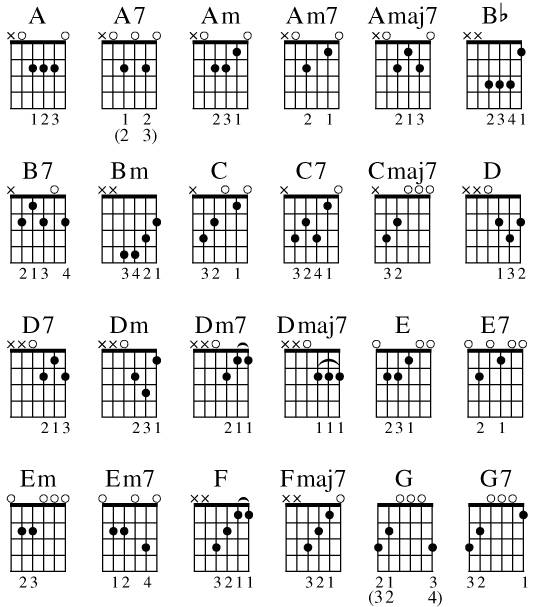
\includegraphics[height=\textheight]{imgs/akordi}
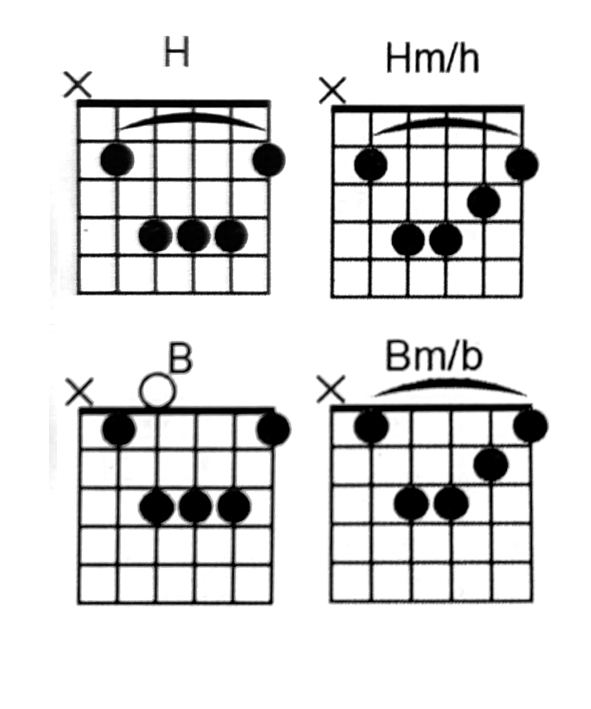
\includegraphics[]{imgs/nemskiAkordi}
\pagebreak


\begin{akordi}

    Fun fact:
    Najpogostejše akorde v tej pesmarci so:
    G (16\%), C(15\%), D (11\%), F (8\%), A in Am (7 \%), E in Em (5\%), Dm (3\%), Hm in F#m (2\%)

    Fun fact 2:
    Najpogostejši glasbeniki: Taborniška, Mi2, Vlado Kreslin, Big foot mama, Zmelkoow, Adi Smolar


\end{akordi}






    \clearpage
\vspace*{\fill}
\begin{center}
    \begin{minipage}{.6\textwidth}

        \centering
        A še kako ntr dam?

    \end{minipage}
\end{center}
\vfill % equivalent to \vspace{\fill}
\clearpage

\end{document}